\documentclass[3p,sort&compress,review,11pt]{elsarticle}
\bibliographystyle{elsarticle-num-names}
\journal{IJNME}
\usepackage{lmodern,amsmath,amsfonts,amssymb,siunitx,graphicx,diagbox,floatrow,booktabs,gnuplot-lua-tikz,structmech,subcaption,bm}
\usepackage[ruled,vlined,nofillcomment]{algorithm2e}
\setstructmech{linewidth=.4pt}
\usetikzlibrary{shapes,arrows.meta}
\newcommand*{\md}[1]{\mathrm{d}#1}
\newcommand*{\va}[1]{\delta#1}
\newcommand*{\mT}{\mathrm{T}}
\newcommand*{\vfrac}[2]{\dfrac{\va#1}{\va#2}}
\newcommand*{\pfrac}[2]{\dfrac{\partial#1}{\partial#2}}
\newcommand*{\figref}[1]{Fig.~\ref{#1}}
\newcommand*{\eqsref}[1]{Eq.~(\ref{#1})}
\newcommand*{\tabref}[1]{Table~\ref{#1}}
\newcommand*{\mb}{\bm}
\begin{document}
\begin{abstract}
By utilizing a modified Hu-Washizu principle, a new mixed variational framework and a corresponding high-performing four-node membrane element with drilling degrees of freedom, named as GCMQ element, are proposed. In this work, the generalized conforming concept, which is originally proposed within a displacement-based formulation, is now extended to a mixed formulation. The new element is able to handle higher-order displacement, strain, and stress distributions. The interpolations are complete up to second order for stress and strain. The enhanced strain field is optimized so that a complete cubic displacement field can be represented. For numerical integration, a five-point scheme is proposed to minimize computational cost. Compared to other four-node elements in existing literature, numerical examples show that the proposed element has a better performance regarding predictions of both displacements and internal forces, particularly under coarse meshes. The new element is also free from shear locking and volumetric locking. Due to the nature of the mixed framework, the element can be directly used in elastoplastic applications.
\end{abstract}
\begin{keyword}
drilling membrane\sep
mixed finite element\sep
coarse-mesh accuracy\sep
mesh distortion
\end{keyword}
\begin{frontmatter}
\title{A New Drilling Quadrilateral Membrane Element With High Coarse-Mesh Accuracy Using A Modified Hu-Washizu Principle}
\author[add1]{T.~L.~Chang\corref{tlc}}\ead{tlcfem@gmail.com}
\author[add1]{C.-L.~Lee}
\author[add1]{A.~J.~Carr}
\author[add1]{R.~P.~Dhakal}
\author[add1]{S.~Pampanin}
\cortext[tlc]{corresponding author}
\address[add1]{Department of Civil and Natural Resources Engineering, University of Canterbury, Christchurch, NZ, 8041.}
\end{frontmatter}
\section{Introduction}
The study of lower-order membrane elements is one of the focuses throughout the development of finite element methods (FEM). The very first elements \citep[e.g.,][]{Turner1956,Taig1964} were widely used in various applications and later adopted as elementary examples in many FEM textbooks \citep[e.g.,][]{Zienkiewicz2013}. In general, early elements are constructed based on the principle of minimum potential energy and convergence is normally guaranteed with refined mesh grids, provided they could pass the patch test.

It is observed that these elements tend to be overstiff, particularly when subjected to in-plane bending, and do not perform well with distorted geometry and large aspect ratios  \citep{Pian1984,Bergan1985}. Besides, conventional membranes also suffer from two other issues that limit their applications in simulating complex systems. The first problem happens when it comes to model connections between panels and beam-type elements, as traditional finite elements only have two degrees of freedom (DoFs) per node while beams possess additional rotational DoFs. The second problem arises in the construction of some planar shell elements by combining membranes and plates together. Since the in-plane rotation DoF is absent, the corresponding main diagonal term is always zero, which leads to a singular element stiffness matrix. Although numerically it is possible to obtain usable elements by modifying zero terms, the additional coupling effects between in-plane and out-of-plane actions cannot be properly captured. This could be a severe problem with coarse mesh configurations.

One possible solution is to introduce in-plane rotational degrees of freedom (also known as drilling DoFs) into element formulation. Initial research on drilling membranes was carried out in 1960's \citep{Felippa1966,Scordelis1967,Willam1969}. The very first application in structural analysis can be traced back to the work by \citet{MacLeod1969}. Successful attempts were later made by others using higher order shape functions \citep{Allman1984,Allman1988,Bergan1985,Cook1986,MacNeal1988}. The interpolation scheme used in Allman's element was also adopted by \citet{Sze1992}, in which, instead of the displacement-based formulation, a two-field Hellinger-Reissner type formulation was used. It did give a more accurate result but additional treatments were required to suppress spurious energy modes. Apart from Allman's method, \citet{Long1994} employed a different interpolation scheme via a generalized conforming approach. From a mathematical perspective, \citet{Hughes1989} managed to derive a special variational principle, in which drilling DoFs are bonded to the nodal rotation that is treated as an independent field. The corresponding element was evaluated by \citet{Hughes1995}. The same principle was also employed by others \citep{Ibrahimbegovic1990,Ibrahimbegovic1992,Ibrahimbegovic1993,Ibrahimbegovic1994,Chinosi1997}. A similar concept was later adopted by \citet{Choi2002} in the derivation of a displacement-based element. Recent explorations can be spotted in the work by \citet{Fajman2002,Cen2011,Cen2015,Madeo2012,Madeo2014,Shang2017}.

Although some superior performance can be obtained \citep[e.g.,][]{Choi2006,Choo2006,Cen2011}, most existing elements are constructed using the (modified) Hellinger-Reissner principle or the minimum complementary energy principle. Two main drawbacks cannot be ignored in those formulations: 1) there are difficulties to use those elements in non-linear plastic applications and 2) additional artificial parameters ($\gamma$ in \citep{Hughes1989} for example), the determination of which is normally empirical, may exist. For recent approaches, such as establishing compatibility between different strains using stresses as weights \citep{Wang2016,Shang2017}, since interpolation functions involve material stiffness, whether those elements can be used in non-linear applications remains unclear. Meanwhile, the overall performance could be further improved.

The ideal membrane element that could address those shortcomings, as well as the ones inherited from classic membranes, is expected to: 1) have only four corner nodes (for smaller matrix bandwidth), 2) possess drilling degrees of freedom, 3) be general for elasto-plastic applications, 4) exhibit excellent performance particularly with coarse meshes, 5) be insensitive to mesh distortion, shear locking and volumetric locking and 6) simplify stress/strain recovery. In this paper, to satisfy those requirements, a four-node drilling membrane element called GCMQ is proposed via a mixed approach based on a modified Hu-Washizu variational principle.

This paper first discusses the definition of degrees of freedom and the decomposition of deformation, followed by a general introduction of the three-field Hu-Washizu variational basis. Based on these two aspects, a modified variational theorem is proposed to establish a proper relationship between different displacement actions. In what follows, a revised solving procedure and a simple, non-iterative algorithm are summarized for element level state determination. The interpolations of all fields are then discussed. Finally, several numerical examples and discussions, in which the proposed element shows a good performance, are presented in corresponding sections.
\section{Deformation Decomposition}
\subsection{Definition of Degrees of Freedom}
For quadrilaterals, strictly speaking, there should be at least four DoFs per node (two for translations and two for independent distortions of both connected edges) to properly describe random deformation. But accounting for the compatibility with other existing elements, in this work, as a common practice, three DoFs are defined for each node: two for translation (denoted by $\mb{u}$ and $\mb{v}$) and one for rotation (denoted by $\mb{\theta}$).

Previous research mainly provides two simple definitions of the drilling DoF $\mb{\theta}$: 1) nodal rigid body rotation \citep{Allman1984} and 2) skew part of strain tensor \citep[e.g.,][]{Hughes1989,Ibrahimbegovic1990,Ibrahimbegovic1992,Ibrahimbegovic1993,Boutagouga2016}. However, those definitions have their own limitations, especially when it comes to the fully-fixed boundary condition in which case both fail to give zero value for drilling DoF. Hence a more appropriate definition should be introduced. Meanwhile, drilling displacement is expected to be decoupled from translation to simplify element formulation. By accounting for above aspects, a definition similar to the one used by \citet{Sze1992} and \citet{Long1994} is adopted in this work. An exhaustive discussion of different definitions of $\mb{\theta}$ can be found elsewhere \citep{Long2009}. A derivation is provided as follows to complete the definition of DoFs.
\subsection{Derivation of Independent Rotation Field}
Let $\mb{F}:\mb{X}\rightarrow\mb{x}$ be a deformation, which is independent of time $t$. Accordingly, the current deformed configuration $\mb{x}\in\mathbb{R}^2$ can be interpreted as the result of applying mapping $\mb{F}$ to the undeformed configuration $\mb{X}\in\mathbb{R}^2$, that is
\begin{gather}\label{eq:mapping}
\mb{x=F\left(X\right)}.
\end{gather}
Similar to the multiplicative decomposition, it is feasible to decompose $\mb{F}$ into two phases. The first one is produced by translational DoFs, namely the translational part. The second one is generated by drilling DoFs, namely the drilling/distortion part. Let $\mb{T}$ and $\mb{D}$ denote these two parts, respectively. Then $\mb{F}$ can be expressed as
\begin{gather*}
\mb{F=D\circ{}T}.
\end{gather*}

Let $\mb{x}_m$ denote the intermediate configuration that is obtained by solely applying mapping $\mb{T}$ to $\mb{X}$,
\begin{gather*}
\mb{x}_m=\mb{T}\left(\mb{X}\right)=\mb{X}+\mb{u}_t\left(\mb{X}\right),
\end{gather*}
in which $\mb{u}_t$ is the translational deformation purely induced by the mapping $\mb{T}$. Then $\mb{x}$ can be expressed as a function of the intermediate configuration $\mb{x}_m$, through the mapping $\mb{D}$,
\begin{gather*}
\mb{x}=\mb{D}\left(\mb{x}_m\right)=\mb{x}_m+\mb{u}_d\left(\mb{x}_m\right).
\end{gather*}

Hence \eqsref{eq:mapping} can be expanded as
\begin{gather}\label{eq:decompose_mapping}
\mb{x}=\mb{F}\left(\mb{X}\right)=\mb{D}\left(\mb{T}\left(\mb{X}\right)\right)=\mb{X}+\mb{u}_t\left(\mb{X}\right)+\mb{u}_d\left(\mb{X}+\mb{u}_t\left(\mb{X}\right)\right).
\end{gather}
By using the Taylor series, one can expand the last term in \eqsref{eq:decompose_mapping} at $\mb{X}$ and obtain
\begin{gather*}
\mb{x}=\mb{X}+\mb{u}_t\left(\mb{X}\right)+\mb{u}_d\left(\mb{X}\right)+\nabla\mb{u}_d\left(\mb{X}\right)\cdot\mb{u}_t\left(\mb{X}\right)+o\left(\mb{u}_t\left(\mb{X}\right)\right),
\end{gather*}
where $\mb{u}_d$ is the drilling deformation and the last term is the Peano's remainder that stands for an infinitesimal term of higher order than $\mb{u}_t$. Within the framework of infinitesimal strain theory, it is reasonable to assume the deformation is sufficiently smooth that $\nabla\mb{u}_d\cdot\mb{u}_t$ is also an infinitesimal of higher order than both $\mb{u}_t$ and $\mb{u}_d$, which themselves are again higher order infinitesimals of $\mb{X}$. For simplicity, it is feasible to discard it, along with the remainder. By such, the total displacement field $\mb{u}$ can be simply written as
\begin{gather}\label{eq:decompose_deformation}
\mb{u}:=\mb{x}-\mb{X}=\mb{u}_t+\mb{u}_d.
\end{gather}
That is to say, the additional drilling deformation caused by the translational deformation is discarded, thus $\mb{u}_t$ and $\mb{u}_d$ can be deemed as independent of each other. The graphical interpretation can be seen in \figref{fig:decompose_deformation}. Such a decomposition cannot be applied in finite deformation problems, in which $\nabla\mb{u}_d\cdot\mb{u}_t$ could be significantly large. The decoupled displacement is important as it allows a great flexibility in the corresponding constructions of interpolations.
\begin{figure}[H]
\centering\scriptsize
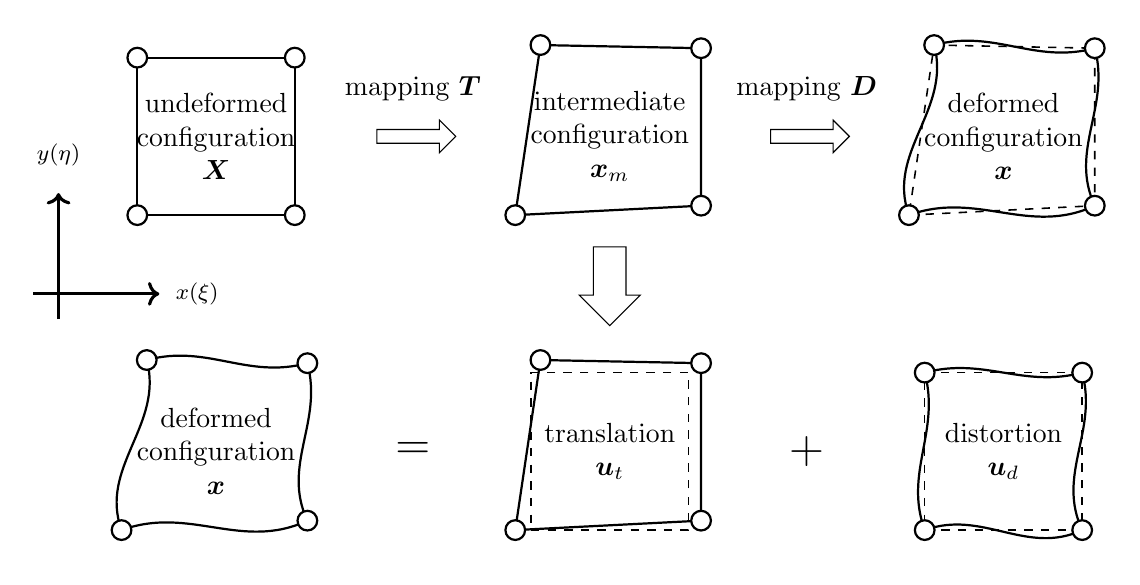
\begin{tikzpicture}[x=2mm,y=2mm]
\def\a{0+20}\def\b{180+25}\def\c{270+15}\def\d{360+15}
\CoorOrigin{-5,-5}[x(\xi)][y(\eta)]{8}
\node[single arrow,draw,minimum height=10mm,single arrow head extend=1.2mm,inner sep=.8mm]at(17.5,5){};
\node[single arrow,draw,minimum height=10mm,single arrow head extend=1.2mm,inner sep=.8mm]at(42.5,5){};
\node[align=center]at(17.5,8){mapping $\mb{T}$};
\node[align=center]at(42.5,8){mapping $\mb{D}$};
\node[single arrow,draw,minimum height=10mm,single arrow head extend=1.8mm,inner sep=2mm,shape border rotate=270]at(30,-4){};
%\node at(15,5){\LARGE$=$};
\node at(17.5,-15){\LARGE$=$};
\node at(42.5,-15){\LARGE$+$};
%\node[align=center]at(5,5){deformed\\configuration\\$\mb{X}$};
\node[align=center]at(5,5){undeformed\\configuration\\$\mb{X}$};
\node[align=center]at(30,5){intermediate\\configuration\\$\mb{x}_m$};
\node[align=center]at(55,5){deformed\\configuration\\$\mb{x}$};
\node[align=center]at(5,-15){deformed\\configuration\\$\mb{x}$};
\node[align=center]at(30,-15){translation\\$\mb{u}_t$};
\node[align=center]at(55,-15){distortion\\$\mb{u}_d$};
%\begin{scope}[every node/.style={circle,thick,draw,fill=white,inner sep=0,minimum size=2.5mm}]
%\draw[thick]
%(0-1,0)node{}to[out=\a,in=\b]
%(10+.8,0+.6)node{}to[out=\b-90,in=\c]
%(10+.8,10+.6)node{}to[out=\c-90,in=\d]
%(0+.6,10+.8)node{}to[out=\d-90,in=\a+90]cycle;
%\end{scope}
\begin{scope}[xshift=00mm,every node/.style={circle,thick,draw,fill=white,inner sep=0,minimum size=2.5mm}]
\draw[thick]
(0,0)node{}--(10,0)node{}--(10,10)node{}--(0,10)node{}--cycle;
\end{scope}
\begin{scope}[xshift=50mm,every node/.style={circle,thick,draw,fill=white,inner sep=0,minimum size=2.5mm}]
\draw[thick]
(0-1,0)node{}--(10+.8,0+.6)node{}--(10+.8,10+.6)node{}--(0+.6,10+.8)node{}--cycle;
\end{scope}
\begin{scope}[xshift=100mm,every node/.style={circle,thick,draw,fill=white,inner sep=0,minimum size=2.5mm}]
\draw[dashed,line width=.2mm]
(0-1,0)--(10+.8,0+.6)--(10+.8,10+.6)--(0+.6,10+.8)--cycle;
\draw[thick]
(0-1,0)node{}to[out=\a,in=\b]
(10+.8,0+.6)node{}to[out=\b-90,in=\c]
(10+.8,10+.6)node{}to[out=\c-90,in=\d]
(0+.6,10+.8)node{}to[out=\d-90,in=\a+90]cycle;
\end{scope}
\begin{scope}[xshift=00mm,yshift=-40mm,every node/.style={circle,thick,draw,fill=white,inner sep=0,minimum size=2.5mm}]
\draw[thick]
(0-1,0)node{}to[out=\a,in=\b]
(10+.8,0+.6)node{}to[out=\b-90,in=\c]
(10+.8,10+.6)node{}to[out=\c-90,in=\d]
(0+.6,10+.8)node{}to[out=\d-90,in=\a+90]cycle;
\end{scope}
\begin{scope}[xshift=50mm,yshift=-40mm,every node/.style={circle,thick,draw,fill=white,inner sep=0,minimum size=2.5mm}]
\draw[dashed,line width=.2mm]
(0,0)--(10,0)--(10,10)--(0,10)--cycle;
\draw[thick]
(0-1,0)node{}--(10+.8,0+.6)node{}--(10+.8,10+.6)node{}--(0+.6,10+.8)node{}--cycle;
\end{scope}
\begin{scope}[xshift=100mm,yshift=-40mm,every node/.style={circle,thick,draw,fill=white,inner sep=0,minimum size=2.5mm}]
\draw[dashed,line width=.2mm]
(0,0)--(10,0)--(10,10)--(0,10)--cycle;
\draw[thick]
(0,0)node{}to[out=\a,in=\b]
(10,0)node{}to[out=\b-90,in=\c]
(10,10)node{}to[out=\c-90,in=\d]
(0,10)node{}to[out=\d-90,in=\a+90]cycle;
\end{scope}
\end{tikzpicture}
% Final.
\caption{deformation decomposition.}\label{fig:decompose_deformation}
\end{figure}
\section{Variational Basis}
\subsection{The Hu-Washizu Principle}
The general form of the Hu-Washizu variational principle \citep{Hu1954} can be written as
\begin{gather*}
\varPi_{HW}\left(\mb{u},\mb{\varepsilon},\mb{\sigma}\right)=\int_V{}\left[W\left(\mb{\varepsilon}\right)+\mb{\sigma}^\mT\left(\nabla\mb{u}-\mb{\varepsilon}\right)\right]\md{V}-\int_V\mb{b}^\mT\mb{u}\md{V}-\int_{S_\sigma}\bar{\mb{t}}^\mT\mb{u}\md{S}-\int_{S_u}\mb{t}^\mT\left(\mb{u}-\bar{\mb{u}}\right)\md{S},
\end{gather*}
in which $V$ denotes the volume domain, $S_\sigma$ and $S_u$ denote the corresponding boundaries, $W\left(\mb{\varepsilon}\right)$ is the strain energy that is normally a non-linear function of the strain $\mb{\varepsilon}$, $\mb{\sigma}$ is the stress, $\mb{u}$ is the displacement field and $\bar{\mb{u}}$ is the prescribed boundary displacement. For brevity, it is feasible to replace the body force $\mb{b}$ term and the boundary traction $\bar{\mb{t}}$ term with the symbol
\begin{gather*}
\varPi_{bt}\left(\mb{u}\right)=\int_V\mb{b}^\mT\mb{u}\md{V}+\int_{S_\sigma}\bar{\mb{t}}^\mT\mb{u}\md{S},
\end{gather*}
since they are normally represented by the equivalent nodal loads that can be treated separately. Meanwhile, an additional field, called the enhanced strain $\hat{\mb{\varepsilon}}$, can be included to further tune element performance. Accounting for above aspects, the following simplified version $\varPi_S$, can be obtained.
\begin{equation}\label{eq:hu_washizu_simplified}
\varPi_S\left(\mb{u},\mb{\varepsilon},\hat{\mb{\varepsilon}},\mb{\sigma}\right)=\int_V\left[W\left(\mb{\varepsilon}\right)+\mb{\sigma}^\mT\left(\nabla\mb{u}+\hat{\mb{\varepsilon}}-\mb{\varepsilon}\right)\right]\md{V}-\int_{S_u}\mb{t}^\mT\left(\mb{u}-\bar{\mb{u}}\right)\md{S}-\varPi_{bt}\left(\mb{u}\right).
\end{equation}
\subsection{A Modified Variational Principle}
It has been shown in \eqsref{eq:decompose_deformation} that the displacement field $\mb{u}$ can be decomposed into two independent portions $\mb{u}_t$ and $\mb{u}_d$ over the problem domain. By definition, the drilling portion $\mb{u}_d$ should be related to the in-plane rotation field $\mb{\theta}$ via certain relationship. Similar to beam elements, one may directly express $\mb{\theta}$ as a function of $\nabla\mb{u}_d$. If so, as the conformity requires $\mb{\theta}$ to be continuous on element boundaries, $\mb{u}_d$ has to be a two dimensional interpolation with $C_1$ continuity. It is commonly known to be very difficult to construct such a function.

Instead of directly imposing the conforming condition, it is possible to handle those two requirements (conformity and $C_1$ continuity) separately. Noting that the $C_1$ continuity is only required on element boundaries, an auxiliary field, denoted by $\mb{u}_\theta$, that is a one-dimensional $C_1$ continuous function of $\mb{\theta}$ and resides only on boundaries, could be introduced. By such, the original $\mb{u}_d$ could simply be interpolated by any two-dimensional function and does not have to be conforming.

It could be noted that a proper interpolation for the translational displacement $\mb{u}_t$ could always be found so that
\begin{gather}\label{eq:boundary_displacement}
\mb{u}_t+\mb{u}_\theta=\bar{\mb{u}}\qquad\text{on $S_u$},
\end{gather}
given that $\mb{u}_\theta$ is already conforming by construction. By inserting \eqsref{eq:boundary_displacement} and \eqsref{eq:decompose_deformation} into \eqsref{eq:hu_washizu_simplified}, one obtains a new functional $\varPi_D$,
\begin{gather}\label{eq:modified_principle}
\varPi_D=\int_V\left[W\left(\mb{\varepsilon}\right)+\mb{\sigma}^\mT\left(\nabla\mb{u}+\hat{\mb{\varepsilon}}-\mb{\varepsilon}\right)\right]\md{V}+\int_{S_u}\mb{t}^\mT\left(\mb{u}_\theta-\mb{u}_d\right)\md{S}-\varPi_{bt},
\end{gather}
with $\mb{u}=\mb{u}_t+\mb{u}_d$ and the conforming condition $\mb{u}_t+\mb{u}_\theta=\bar{\mb{u}}$ on $S_u$ as an essential condition. The displacement boundary $S_u$ term in the above functional, viz.,
\begin{gather}\label{eq:constraint}
\int_{S_u}\mb{t}^\mT\left(\mb{u}_\theta-\mb{u}_d\right)\md{S},
\end{gather}
acts as a minimum conformity constraint imposed on $\mb{u}_d$ and $\mb{u}_\theta$ that guarantees convergence.
\section{Element Formulation}
\subsection{A Simplification}
\eqsref{eq:constraint} can be further relaxed by noting that when element size approaches zero, the corresponding traction $\mb{t}$ approaches a constant field that can be denoted as $\mb{t}_c$. In which case, \eqsref{eq:constraint} can be rewritten as
\begin{gather*}
\int_{S_u}\mb{t}_c^\mT\left(\mb{u}_\theta-\mb{u}_d\right)\md{S}=\mb{t}_c^\mT\int_{S_u}\left(\mb{u}_\theta-\mb{u}_d\right)\md{S}.
\end{gather*}
To avoid treating $\mb{u}_d$ separately, a slightly stronger constraint can be applied, for example,
\begin{gather}\label{eq:conforming_constraint_simplified}
\int_{S_i}\mb{I}\left(\mb{u}_d-\mb{u}_\theta\right)\md{S}=\mb{0}\quad\text{for $i=1,2,3,4$},
\end{gather}
where $\mb{I}$ is the \numproduct{2x2} identity matrix. It should be noted that \eqsref{eq:conforming_constraint_simplified} is applied on four edges separately, hence instead of one, eight independent constraints (two for each edge) are provided. \eqsref{eq:conforming_constraint_simplified} is in fact identical to the constraint used in GQ12 element \citep{Long1994}. This approach is known as the generalized conforming method that can be initially observed in the work by \citet{Tang1984} and \citet{Wu1987} and later utilized,  further enriched by \citet{Long1994}. Physically it means $\mb{u}_d$ and $\mb{u}_\theta$ are equivalent to each other in a weak sense on each element boundary.

In a more generic setup, \eqsref{eq:conforming_constraint_simplified} can be rewritten as
\begin{gather}\label{eq:conforming_constraint_full}
\int_{S_i}\mb{S}^n\left(\mb{u}_d-\mb{u}_\theta\right)\md{S}=\mb{0}\quad\text{for $i=1,2,3,4$},
\end{gather}
in which $\mb{S}=\mathrm{diag}(S,~S)$. \eqsref{eq:conforming_constraint_simplified} is a special case of \eqsref{eq:conforming_constraint_full} with $n=0$.

Let $\mb{d}$ denote the generalised interpolation parameter used in $\mb{u}_d$ and assume $\mb{u}_\theta$ to be a function of nodal rotation $\mb{\theta}$, it is possible to express $\mb{d}$ as a function of $\mb{\theta}$ by solving \eqsref{eq:conforming_constraint_simplified},
\begin{gather*}
\mb{u}_d=f_1\left(\mb{d}\right)=f_1\left(f_2\left(\mb{\theta}\right)\right)=f_3\left(\mb{\theta}\right),
\end{gather*}
although solution is not guaranteed and it also depends on the discrete form of $\mb{u}_d$, this part will be discussed in the subsequent section. By such, the displacement $\mb{u}$ can be expressed solely by nodal translations and rotations. Meanwhile, \eqsref{eq:conforming_constraint_simplified} implies that \eqsref{eq:constraint} equals to zero in a generalised conforming sense. Hence, the governing variational principle \eqsref{eq:modified_principle} falls back to
\begin{gather}\label{eq:final_principle}
\varPi_F\left(\mb{u},\mb{\varepsilon},\hat{\mb{\varepsilon}},\mb{\sigma}\right)=\int_V\left[W\left(\mb{\varepsilon}\right)+\mb{\sigma}^\mT\left(\nabla\mb{u}+\hat{\mb{\varepsilon}}-\mb{\varepsilon}\right)\right]\md{V}-\varPi_{bt}\left(\mb{u}\right),
\end{gather}
which is adopted in the formulation of the new element. It should be mentioned that \eqsref{eq:conforming_constraint_simplified} is not the only option. \eqsref{eq:constraint} could be replaced by various generalised conforming schemes. The interested readers are referred to the monograph \citep{Long2009} for more details.
\subsection{Solving Equations}
Since the finally adopted functional is \eqsref{eq:final_principle}, the solving procedure of which has already been given elsewhere \citep{Piltner1995,Piltner1999}, here only a brief summary is presented. Nevertheless, it shall still be noted that in the following derivation, unlike the original literature, the symmetry requirement is imposed on neither material stiffness nor any other matrices. Meanwhile, the state updating scheme is also corrected so that a stable algorithm is obtained.

Taking variations of \eqsref{eq:hu_washizu_simplified} gives,
\begin{equation}\label{eq:euler_equation}
\left\{\begin{array}{l}
\displaystyle\int_V\va{\left(\nabla\mb{u}\right)}^\mT\mb{\sigma}~\md{V}=\va{\mb{u}}^\mT\vfrac{\varPi_{bt}}{\mb{u}},\\[3mm]
\displaystyle\int_V\va{\mb{\sigma}}^\mT\left(\nabla\mb{u}+\hat{\mb{\varepsilon}}-\mb{\varepsilon}\right)~\md{V}=0,\\[3mm]
\displaystyle\int_V\va{\mb{\varepsilon}}^\mT\left(\tilde{\mb{\sigma}}\left(\mb{\varepsilon}\right)-\mb{\sigma}\right)~\md{V}=0,\\[3mm]
\displaystyle\int_V\va{\hat{\mb{\varepsilon}}}^\mT\mb{\sigma}~\md{V}=0,
\end{array}\right.
\end{equation}
where $\tilde{\mb{\sigma}}\left(\mb{\varepsilon}\right)=\partial{}W\left(\mb{\varepsilon}\right)/\partial\mb{\varepsilon}$ is the stress obtained from material model. By discretising four independent fields with
\begin{gather*}
\mb{u}=\mb{\phi}_u\mb{q},\quad
\mb{\sigma}=\mb{\phi}_\sigma\mb{\alpha},\quad
\mb{\varepsilon}=\mb{\phi}_\varepsilon\mb{\beta},\quad
\hat{\mb{\varepsilon}}=\mb{\phi}_{\hat{\varepsilon}}\mb{\zeta},
\end{gather*}
\eqsref{eq:euler_equation} can also be expressed as
\begin{gather}\label{eq:discretised_euler_equation}
\left\{\begin{array}{l}
\displaystyle\va{\mb{q}^\mT}\int_V\left(\mb{L}\mb{\phi}_u\right)^\mT\mb{\phi}_\sigma\mb{\alpha}~\md{V}=\va{\mb{q}}^\mT\vfrac{\varPi_{bt}}{\mb{q}}=\va{\mb{q}}^\mT\mb{P},\\[3mm]
\displaystyle\va{\mb{\alpha}^\mT}\int_V\mb{\phi}_\sigma^\mT\left(\mb{L}\mb{\phi}_u\mb{q}+\mb{\phi}_{\hat{\varepsilon}}\mb{\zeta}-\mb{\phi}_\varepsilon\mb{\beta}\right)~\md{V}=0,\\[3mm]
\displaystyle\va{\mb{\beta}^\mT}\int_V\mb{\phi}_\varepsilon^\mT\left(\tilde{\mb{\sigma}}\left(\mb{\varepsilon}\right)-\mb{\phi}_\sigma\mb{\alpha}\right)~\md{V}=0,\\[3mm]
\displaystyle\va{\mb{\zeta}^\mT}\int_V\mb{\phi}_{\hat{\varepsilon}}^\mT\mb{\phi}_\sigma\mb{\alpha}~\md{V}=0.
\end{array}\right.
\end{gather}
The corresponding linearised equations between two adjacent iterations denoted with pseudo-time $t_n$ and $t_{n+1}$ could be obtained as
\begin{equation}
\left\{\begin{array}{l}
\displaystyle\int_V\left(\mb{L}\mb{\phi}_u\right)^\mT\mb{\phi}_\sigma\Delta\mb{\alpha}~\md{V}=\mb{P}_{n+1}-\mb{P}_n,\\[3mm]
\displaystyle\int_V\mb{\phi}_\sigma^\mT\left(\mb{L}\mb{\phi}_u\Delta\mb{q}+\mb{\phi}_{\hat{\varepsilon}}\Delta\mb{\zeta}-\mb{\phi}_\varepsilon\Delta\mb{\beta}\right)~\md{V}=\mb{0},\\[3mm]
\displaystyle\int_V\mb{\phi}_\varepsilon^\mT\left(\tilde{\mb{E}}\mb{\phi}_\varepsilon\Delta\mb{\beta}-\mb{\phi}_\sigma\Delta\mb{\alpha}\right)~\md{V}=-\mb{Q}_n,\\[3mm]
\displaystyle\int_V\mb{\phi}_{\hat{\varepsilon}}^\mT\mb{\phi}_\sigma\Delta\mb{\alpha}~\md{V}=-\mb{F}_n,
\end{array}\right.
\end{equation}
in which $\mb{P}_{n+1}$ stands for the external load that could include contributions of nodal forces, body forces and/or surface tractions. The increment of material stress $\Delta\tilde{\mb{\sigma}}$ is linearised with tangent stiffness $\tilde{\mb{E}}$ that could also be obtained from material model,
\begin{gather}
\Delta\tilde{\mb{\sigma}}\approx\tilde{\mb{E}}\Delta\mb{\varepsilon}=\tilde{\mb{E}}\mb{\phi}_\varepsilon\Delta\mb{\beta}.
\end{gather}
The gradient operator $\mb{L}$ could be expressed as
\begin{gather*}
\mb{L}=\begin{bmatrix}
\partial/\partial{}x&\cdot&\partial/\partial{}y\\[3mm]
\cdot&\partial/\partial{}y&\partial/\partial{}x
\end{bmatrix}^\mT,
\end{gather*}
where $x$ and $y$ are global coordinates. Resistance $\mb{P}_n$, residuals $\mb{Q}_n$ and $\mb{F}_n$ are
\begin{gather}
\mb{P}_n=\int_V\left(\mb{L}\mb{\phi}_u\right)^\mT\mb{\phi}_\sigma\mb{\alpha}_n\md{V},\\
\mb{Q}_n=\int_V\mb{\phi}_\varepsilon^\mT\tilde{\mb{\sigma}}_n-\mb{\phi}_\varepsilon^\mT\mb{\phi}_\sigma\mb{\alpha}_n~\md{V},\\
\mb{F}_n=\int_V\mb{\phi}_{\hat{\varepsilon}}^\mT\mb{\phi}_\sigma\mb{\alpha}_n\md{V}.
\end{gather}
The non-zero term $\mb{F}_n$ origins from a relaxed version of the fourth equation in \eqsref{eq:euler_equation}, which represents a full orthogonality condition that should be enforced on enhanced strain $\hat{\mb{\varepsilon}}$ so that the resulting element could pass the patch test \citep{Simo1990}. However, with such a condition, it is difficult to recover the magnitude of $\hat{\mb{\varepsilon}}$. Hence, instead of the original condition, a partially orthogonal one can be adopted \citep{Piltner1995}, that is
\begin{gather*}
\int_V\va{\hat{\mb{\varepsilon}}}^\mT\hat{\mb{\sigma}}\md{V}=0,
\end{gather*}
in which $\hat{\mb{\sigma}}$ is a reference stress field consists of at least three constant modes. If the adopted stress interpolation employs higher order polynomials, the original expression does not necessarily equal to zero for all non-converged iterations.

By further denoting
\begin{gather}
%\begin{array}{llll}
\mb{H}=\int_{V}\mb{\phi}_\sigma^\mT\mb{\phi}_\varepsilon\md{V},\quad
\tilde{\mb{H}}=\int_{V}\mb{\phi}_\varepsilon^\mT\tilde{\mb{E}}\mb{\phi}_\varepsilon\md{V},\quad
\mb{M}=\int_{V}\mb{\phi}_\sigma^\mT\mb{\phi}_{\hat{\varepsilon}}\md{V},\quad
\mb{N}=\int_{V}\mb{\phi}_\sigma^\mT\mb{L}\mb{\phi}_u\md{V},
%\end{array}
\end{gather}
the system of linear equations can be obtained as
\begin{gather}\label{eq:solving_system}
\begin{bmatrix}
	\cdot        & \mb{N}^\mT  & \cdot                & \cdot        \\
	\mb{N} & \cdot             & -\mb{H}        & \mb{M} \\
	\cdot        & -\mb{H}^\mT & \tilde{\mb{H}} & \cdot        \\
	\cdot        & \mb{M}^\mT  & \cdot                & \cdot
\end{bmatrix}\begin{bmatrix}
\Delta\mb{q}\\\Delta\mb{\alpha}\\\Delta\mb{\beta}\\\Delta\mb{\zeta}
\end{bmatrix}=\begin{bmatrix}
\mb{P}_{n+1}-\mb{P}_n\\\mb{0}\\-\mb{Q}_n\\-\mb{F}_n
\end{bmatrix}.
\end{gather}
\subsection{Solution Procedure}
The traditional local iterative scheme can be adopted for solving \eqsref{eq:solving_system}. From the third equation in \eqsref{eq:solving_system}, $\Delta\mb{\beta}$ can be expressed as
\begin{gather*}
\Delta\mb{\beta}=\tilde{\mb{H}}^{-1}\left(\mb{H}^\mT\Delta\mb{\alpha}-\mb{Q}_n\right),
\end{gather*}
assuming $\tilde{\mb{H}}$ is invertible, inserting it into the second equation, one obtains
\begin{gather*}
\Delta\mb{\alpha}=\left(\mb{H}\tilde{\mb{H}}^{-1}\mb{H}^\mT\right)^{-1}\left(\mb{N}\Delta\mb{q}+\mb{M}\Delta\mb{\zeta}+\mb{H}\tilde{\mb{H}}^{-1}\mb{Q}_n\right).
\end{gather*}

However, if $\mb{H}$ is square and invertible, the stress interpolation parameter $\mb{\alpha}$ could be directly updated according to the third equation in \eqsref{eq:discretised_euler_equation}, that is
\begin{gather}\label{eq:answer_alpha}
\mb{\alpha}=\mb{H}^{-\mT}\int_V\mb{\phi}_\varepsilon^\mT\tilde{\mb{\sigma}}\md{V}.
\end{gather}
It could be seen that $\mb{\alpha}$ only depends on material stress $\tilde{\mb{\sigma}}$ and can be computed immediately after updating material state. Since stress equilibrium is enforced (by selecting proper stress field, as can be seen later), the corresponding residual simply equals to zero,
\begin{gather*}
\mb{Q}_n=\mb{0}.
\end{gather*}
Meanwhile, $\Delta\mb{\beta}$ can be directly obtained from the second equation as
\begin{gather}\label{eq:answer_beta}
\Delta\mb{\beta}=\tilde{\mb{N}}\Delta\mb{q}+\tilde{\mb{M}}\Delta\mb{\zeta},
\end{gather}
in which $\tilde{\mb{N}}=\mb{H}^{-1}\mb{N}$ and $\tilde{\mb{M}}=\mb{H}^{-1}\mb{M}$.

The remaining equations can be rearranged as
\begin{gather*}
\begin{bmatrix}
\mb{U}&\mb{W}\\\mb{W}^\mT&\mb{V}
\end{bmatrix}
\begin{bmatrix}
\Delta\mb{q}\\\Delta\mb{\zeta}
\end{bmatrix}=
\begin{bmatrix}
\mb{P}_{n+1}-\mb{P}_n\\-\mb{F}_n
\end{bmatrix},
\end{gather*}
in which
\begin{gather}\label{eq:answer_uvw}
\mb{U}=\tilde{\mb{N}}^\mT\tilde{\mb{H}}\tilde{\mb{N}},\quad
\mb{V}=\tilde{\mb{M}}^\mT\tilde{\mb{H}}\tilde{\mb{M}},\quad
\mb{W}=\tilde{\mb{N}}^\mT\tilde{\mb{H}}\tilde{\mb{M}}.
\end{gather}

By repeating the same condensation procedure, one could obtain
\begin{gather}\label{eq:answer_zeta}
\Delta\mb{\zeta}=\mb{V}^{-1}\left(-\mb{F}_n-\mb{W}^\mT\Delta\mb{q}\right),
\end{gather}
which leads to the final expression of equivalent stiffness $\mb{K}$
\begin{gather}\label{eq:answer_stiffness}
\mb{K}=\mb{U}-\mb{W}\mb{V}^{-1}\mb{W}^\mT,
\end{gather}
while equivalent resistance $\mb{R}$ is
\begin{gather}\label{eq:answer_resistance}
\mb{R}=\mb{P}_n-\mb{W}\mb{V}^{-1}\mb{F}_n.
\end{gather}

It should be noted that the above procedure can largely reduce computation cost but is only valid for an invertible $\mb{H}$. Otherwise a standard condensation should be conducted on \eqsref{eq:solving_system}.
\subsection{Implementation Algorithm}
For state determination at element level, here a non-iterative scheme is presented in Algorithm \ref{algo:adaptive_algorithm} where $w^i$ denotes the generalized numerical integration weight that could include original integration weight, element thickness and determinant of Jacobian at each integration point.

The efficiency of GCMQ is not considered as a problem, especially when it runs with a parallel computation framework on modern computers. Algorithm \ref{algo:adaptive_algorithm} also lists the \textbf{optimized} numbers of arithmetic multiplications required for each manipulation with one enhanced strain mode. The total cost of GCMQ with a nine-point integration scheme and three enhanced strain modes is similar to the one of Q8 \citep{Ergatoudis1968}. With the same mesh configuration, GCMQ has fewer nodes and DoFs than Q8. This leads to a smaller and narrower global stiffness matrix hence a higher overall efficiency. If other factors such as a five-point integration scheme and/or potentially fewer iterations required for global convergence are considered, the efficiency can be further improved.

\begin{algorithm}[H]
\SetAlgoLined\SetArgSty{}
\SetKw{Return}{return}
\SetKw{Compute}{compute}
\SetKw{Update}{update}
\SetKw{Break}{break}
\KwIn{$\Delta\mb{q}$, $\mb{q}_n$, $\mb{\alpha}_n$, $\mb{\beta}_n$, $\mb{\zeta}_n$, $\mb{V}_n$, $\mb{W}_n$}
\KwOut{$\mb{K}$, $\mb{R}$, $\mb{q}_{n+1}$, $\mb{\alpha}_{n+1}$, $\mb{\beta}_{n+1}$, $\mb{\zeta}_{n+1}$, $\mb{V}_{n+1}$, $\mb{W}_{n+1}$}
$\mb{q}_{n+1}=\mb{q}_n+\Delta\mb{q}$\;
$\Delta\mb{\zeta}=-\mb{V}^{-1}_n\mb{M}^\mT\mb{\alpha}_n-\mb{V}^{-1}_n\mb{W}_n^\mT\Delta\mb{q}$\tcp*[r]{counter: 12 \eqsref{eq:answer_zeta}}
$\Delta\mb{\beta}=\tilde{\mb{N}}\Delta\mb{q}+\tilde{\mb{M}}\Delta\mb{\zeta}$\tcp*[r]{counter: 143 \eqsref{eq:answer_beta}}
$\mb{\zeta}_{n+1}=\mb{\zeta}_n+\Delta\mb{\zeta}$\;
$\mb{\beta}_{n+1}=\mb{\beta}_n+\Delta\mb{\beta}$\;
\ForAll{integration points}{
$\mb{\varepsilon}_{n+1}^i=\mb{\phi}_{\varepsilon}^i\mb{\beta}_{n+1}$\tcp*[r]{counter: 33}
obtain $\tilde{\mb{E}}_{n+1}^i$ and $\tilde{\mb{\sigma}}_{n+1}^i$ from the material model\;
assemble $\displaystyle\tilde{\mb{H}}_{n+1}=\sum{}w^i\mb{\phi}_{\varepsilon}^{i,\mT}\tilde{\mb{E}}_{n+1}^i\mb{\phi}_{\varepsilon}^i$\tcp*[r]{counter: 462}
assemble $\displaystyle\tilde{\mb{S}}_{n+1}=\sum{}w^i\mb{\phi}_\varepsilon^{i,\mT}\tilde{\mb{\sigma}}_{n+1}^i$\tcp*[r]{counter: 33}
}
$\mb{\alpha}_{n+1}=\mb{H}^{-\mT}\tilde{\mb{S}}_{n+1}$\tcp*[r]{counter: 121 \eqsref{eq:answer_alpha}}
update $\mb{U}_{n+1}$, $\mb{V}_{n+1}$ and $\mb{W}_{n+1}$ using $\tilde{\mb{H}}_{n+1}$\tcp*[r]{counter: 1850 \eqsref{eq:answer_uvw}}
$\mb{K}=\mb{U}_{n+1}-\mb{W}_{n+1}\mb{V}^{-1}_{n+1}\mb{W}_{n+1}^\mT$\tcp*[r]{counter: 1716 \eqsref{eq:answer_stiffness}}
$\mb{R}=\mb{N}\mb{\alpha}_{n+1}-\mb{W}_{n+1}\mb{V}_{n+1}^{-1}\mb{M}^\mT\mb{\alpha}_{n+1}$\tcp*[r]{counter: 144 \eqsref{eq:answer_resistance}}
\caption{state determination at element level}\label{algo:adaptive_algorithm}
\end{algorithm}

It should be noted that $\mb{H}$, $\mb{M}$, $\mb{N}$, $\tilde{\mb{M}}$ and $\tilde{\mb{N}}$ are all constant matrices. Once the corresponding shape functions are chosen, they could be readily computed, stored and later used in analysis. Meanwhile, $\mb{U}$, $\mb{V}$ and $\mb{W}$ solely depend on the material tangent $\tilde{\mb{E}}$ that should be computed according to given strain $\mb{\varepsilon}$ and/or other variables. Accordingly, they could be initialized, stored and updated as element level history variables during iterations.
\section{Construction of Interpolations}
\subsection{Displacement}
As a conventional approach, the translational part of displacement field $\mb{u}_t$ is interpolated by nodal translations via an isoparametric mapping, that is,
\begin{gather}
\mb{u}_t=\begin{bmatrix}u_t&v_t\end{bmatrix}^\mT=\mb{\phi}_t\mb{q}_t,
\end{gather}
in which
\begin{gather*}
\mb{\phi}_t=\begin{bmatrix}
N_1&0&N_2&0&N_3&0&N_4&0\\
0&N_1&0&N_2&0&N_3&0&N_4
\end{bmatrix},\\
\mb{q}_t=\begin{bmatrix}
u_1&v_1&u_2&v_2&u_3&v_3&u_4&v_4
\end{bmatrix}^\mT,\\
N_i=\dfrac{1}{4}\left(1+\xi\xi_i\right)\left(1+\eta\eta_i\right)\quad\text{for}\quad{}i=1,2,3,4,
\end{gather*}
with $\xi_i$ and $\eta_i$ are parent coordinates of corresponding nodes.

For the drilling part $\mb{u}_d$, the corresponding shape functions can be in fact arbitrarily chosen as no $C_1$ continuity is imposed.
\begin{gather}\label{eq:interpolation_displacement}
\mb{u}_d=\begin{bmatrix}u_d&v_d\end{bmatrix}^\mT=\mb{\phi}_d\mb{d}.
\end{gather}
Since the bilinear terms have already been included in the translational part, higher order terms could be picked in $\mb{u}_d$. One possible choice is a serendipity-like basis. Mimicking a similar form used for $\mb{\phi}_t$, $\mb{\phi}_d$ can be written as
\begin{gather}
\mb{\phi}_d=\begin{bmatrix}
\bar{N}_1&0&\bar{N}_2&0&\bar{N}_3&0&\bar{N}_4&0\\
0&\bar{N}_1&0&\bar{N}_2&0&\bar{N}_3&0&\bar{N}_4
\end{bmatrix},\\\label{eq:shape_function_displacement}
\begin{array}{llll}
\bar{N}_1=1-\xi^2,&\bar{N}_2=\eta-\xi^2\eta,&\bar{N}_3=1-\eta^2,&\bar{N}_4=\xi-\xi\eta^2.
\end{array}
\end{gather}
Accordingly, $\mb{d}$ consists of eight generalized interpolation parameters that do not need to possess any physical meaning, although with \eqsref{eq:shape_function_displacement}, they correspond to the displacement values of centres of four edges.
\begin{gather*}
\mb{d}=\begin{bmatrix}
d_1&d_2&d_3&d_4&d_5&d_6&d_7&d_8
\end{bmatrix}^\mT.
\end{gather*}

For the boundary version $\mb{u}_\theta$, to satisfy the imposed $C_1$ continuity requirement, it is feasible to choose the Hermite interpolation or other parametric curves (e.g., splines) as the shape functions. Here in this work a Hermite-type curve constructed by two nodal rotations $\theta_i$ are adopted. For each edge $l_j$,
\begin{gather*}
\mb{u}_\theta=\begin{bmatrix}w_j\end{bmatrix}=\sum_{i=1}^{2}\tilde{N}_i\theta_i,
\end{gather*}
in which $w_j$ is the displacement perpendicular to the edge since this is a beam-type interpolation, and
\begin{gather*}
\tilde{N}_1=\dfrac{l_j}{8}\left(s^3-s^2-s+1\right),\quad
\tilde{N}_2=\dfrac{l_j}{8}\left(s^3+s^2-s-1\right),
\end{gather*}
where the edge label $l_j$ is also used to denote the length of that edge and $-1\leqslant{}s\leqslant1$ is the parent coordinate. There are several methods to transform the displacement $w_j$ from the local system to the global one as depicted in \figref{fig:coordinate_system}. Here a simple decomposition is used.
\begin{gather}
\mb{u}_\theta=\begin{bmatrix}u_\theta\\v_\theta\end{bmatrix}=w_j\begin{bmatrix}\cos\left(\psi_j+\dfrac{\pi}{2}\right)\\[2mm]\sin\left(\psi_j+\dfrac{\pi}{2}\right)\end{bmatrix}=w_j\begin{bmatrix}-\sin\psi_j\\[2mm]\cos\psi_j\end{bmatrix}.
\end{gather}
where $\psi_j$ is the inclination of the edge. Other curves may be used as substitutes. Additional internal parameters can also be introduced to further control the deformation.
\begin{figure}[H]
\centering\scriptsize
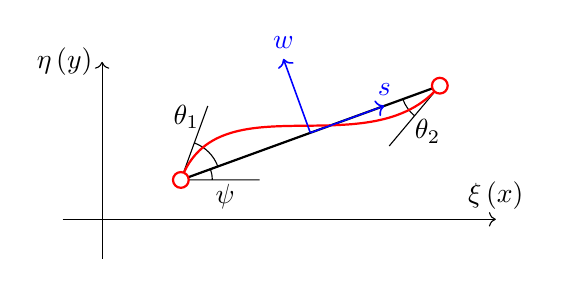
\begin{tikzpicture}
\def\a{20}\def\b{50}\def\c{}
\coordinate(A)at(1,.5);
\coordinate(B)at($(A)+(\a:3.5)$);
\coordinate(C)at($(A)+(\a:1.75)$);
\draw[->](-.5,0)--(5,0)node[anchor=south]{$\xi\left(x\right)$};
\draw[->](0,-.5)--(0,2)node[anchor=east]{$\eta\left(y\right)$};
\draw[thick](A)--(B);
\draw[](A)--+(\a+\b:1)(A)--+(1,0)(A)--+(\a:.5)arc(\a:\a+\b:.5)(A)--+(0:.4)arc(0:\a:.4);
\draw[](B)--+(180+\b:1)(B)--+(180+\a:.5)arc(180+\a:180+\b:.5);
\draw[red,thick](A)node[thick,draw,circle,fill=white,inner sep=0,minimum size=2mm]{}to[in=180+\b,out=\a+\b](B)node[thick,draw,circle,fill=white,inner sep=0,minimum size=2mm]{};
\draw[](A)+(-20:.6)node{$\psi$};
\draw[](A)+(\a+\b/2+40:.8)node{$\theta_1$};
\draw[](B)+(210+\a+\b/2:.6)node{$\theta_2$};
\draw[blue,->,line width=.2mm](C)--+(\a:1)node[anchor=south]{$s$};
\draw[blue,->,line width=.2mm](C)--+(\a+90:1)node[anchor=south]{$w$};
\end{tikzpicture}
\caption{illustration of coordinate systems}\label{fig:coordinate_system}
\end{figure}

Now \eqsref{eq:conforming_constraint_simplified} can be established explicitly. It provides eight independent constraints, which can be expanded as
\begin{gather*}
\int_{S_1}\mb{u}_d~\md{S}=\int_{S_1}\mb{u}_\theta~\md{S},\quad
\int_{S_2}\mb{u}_d~\md{S}=\int_{S_2}\mb{u}_\theta~\md{S},\\
\int_{S_3}\mb{u}_d~\md{S}=\int_{S_3}\mb{u}_\theta~\md{S},\quad
\int_{S_4}\mb{u}_d~\md{S}=\int_{S_4}\mb{u}_\theta~\md{S}.
\end{gather*}
The integrations can be performed analytically for both $\mb{u}_\theta$ and $\mb{u}_d$. By collecting all equations and rearranging them into a matrix form, one obtains
\begin{gather}
\mb{G}\mb{d}=\mb{Q}\mb{\theta},
\end{gather}
with $\mb{\theta}=\begin{bmatrix}\theta_1&\theta_2&\theta_3&\theta_4\end{bmatrix}^\mT$, $\mb{G}$ and $\mb{Q}$ are explicitly shown as in \eqsref{eq:interpolation_conforming}.
\begin{gather}\label{eq:interpolation_conforming}
\underset{\numproduct{8x4}}{\mb{Q}}=\int_{-1}^{1}\text{diag}\begin{pmatrix}
-\sin\psi_1\\\cos\psi_1\\-\sin\psi_2\\\cos\psi_2\\-\sin\psi_3\\\cos\psi_3\\-\sin\psi_4\\\cos\psi_4
\end{pmatrix}\cdot\begin{bmatrix}
\tilde{N}_1&\tilde{N}_2&\cdot&\cdot\\
\tilde{N}_1&\tilde{N}_2&\cdot&\cdot\\
\cdot&\tilde{N}_1&\tilde{N}_2&\cdot\\
\cdot&\tilde{N}_1&\tilde{N}_2&\cdot\\
\cdot&\cdot&\tilde{N}_1&\tilde{N}_2\\
\cdot&\cdot&\tilde{N}_1&\tilde{N}_2\\
\tilde{N}_2&\cdot&\cdot&\tilde{N}_1\\
\tilde{N}_2&\cdot&\cdot&\tilde{N}_1\\
\end{bmatrix}\md{s},\qquad
\underset{\numproduct{8x8}}{\mb{G}}=\begin{bmatrix}
\displaystyle\int_{-1}^{1}\mb{\phi}_d\Big|_{\eta=-1}~\md{\xi}\\[3mm]
\displaystyle\int_{-1}^{1}\mb{\phi}_d\Big|_{\xi=1}~\md{\eta}\\[3mm]
\displaystyle\int_{-1}^{1}\mb{\phi}_d\Big|_{\eta=1}~\md{\xi}\\[3mm]
\displaystyle\int_{-1}^{1}\mb{\phi}_d\Big|_{\xi=-1}~\md{\eta}
\end{bmatrix}.
\end{gather}

Assume $\mb{G}$ is invertible, then
\begin{gather}\label{eq:interpolation_conforming_answer}
\mb{d}=\mb{G}^{-1}\mb{Q}\mb{\theta},
\end{gather}
inserting \eqsref{eq:interpolation_conforming_answer} into \eqsref{eq:interpolation_displacement}, $\mb{u}_d$ can eventually be expressed by $\mb{\theta}$, which consists of four nodal rotations.
\begin{gather}
\mb{u}_d=\mb{\phi}_d\mb{d}=\mb{\phi}_d\mb{G}^{-1}\mb{Q}\mb{\theta}.
\end{gather}

Then \eqsref{eq:decompose_deformation} can be reinterpreted by $\mb{q}_t$ and $\mb{\theta}$,
\begin{gather}
\mb{u}=\mb{u}_t+\mb{u}_d=\mb{\phi}_t\mb{q}_t+\mb{\phi}_d\mb{G}^{-1}\mb{Q}\mb{\theta}.
\end{gather}
Accordingly,
\begin{gather*}
\mb{\phi}_u=\begin{bmatrix}
\mb{\phi}_t&\mb{\phi}_d\mb{G}^{-1}\mb{Q}
\end{bmatrix},\qquad
\mb{q}=\begin{bmatrix}
\mb{q}_t&\mb{\theta}
\end{bmatrix}^\mT.
\end{gather*}
The order of $\mb{q}$ could be rearranged to match corresponding DoF encoding rule. As there is no additional constraint imposed, $\mb{G}$ could be singular, hence a careful construction of $\mb{\phi}_d$ is required to avoid singularity.
\subsection{Stress}
The stress modes can be derived from the Airy stress function, as a common practice that has been used in prior research \citep[see, e.g.,][]{Fu2010,Cen2011,Nodargi2017}.
\begin{gather}
\mb{\sigma}=\begin{bmatrix}
	\sigma_x & \sigma_y & \tau_{xy}
\end{bmatrix}^\mT=\mb{\phi}_\sigma\mb{\alpha},
\end{gather}
with $\mb{\alpha}=\begin{bmatrix}
	\alpha_1 & \alpha_2 & \alpha_3 & \cdots & \alpha_{11}
\end{bmatrix}^\mT$. The shape function $\mb{\phi}_\sigma$ can be explicitly shown as in \eqsref{fig:interpolation_stress},
\begin{gather}\label{fig:interpolation_stress}
\mb{\phi}_\sigma=
\left[\begin{array}{ccc|cc|cc|cc|cc}
	1 & 0 & 0 & 0 & y & 0  & x  &  0   & 2xy  &   -x^2   & 2y^2-x^2 \\
	0 & 1 & 0 & x & 0 & y  & 0  & 2xy  &  0   & 2x^2-y^2 &   -y^2   \\
	0 & 0 & 1 & 0 & 0 & -x & -y & -x^2 & -y^2 &   2xy    &   2xy
\end{array}\right].
\end{gather}
The chosen $\mb{\phi}_\sigma$ is complete up to second order. Compared to the one adopted by \citet{Fu2010}, which can be referred to for a detailed derivation, the last two columns are however different --- a symmetric pair is chosen here. Once the Jacobian matrix is known, $\mb{\sigma}$ can be conveniently expressed as a function of parent coordinates $\xi$ and $\eta$.
\subsection{Strain}
The strain field is interpolated in a similar way,
\begin{gather}
\mb{\varepsilon}=\begin{bmatrix}
	\varepsilon_x & \varepsilon_y & \gamma_{xy}
\end{bmatrix}^\mT=\mb{\phi}_\varepsilon\mb{\beta}=\mb{C}\mb{\phi}_\sigma\mb{\beta},
\end{gather}
with $\mb{\beta}=\begin{bmatrix}
	\beta_1 & \beta_2 & \beta_3 & \cdots & \beta_{11}
\end{bmatrix}^\mT$. For isotropic materials, the constant matrix $\mb{C}$ is chosen to be dependent on Poisson's ratio $\nu$,
\begin{gather}\label{poisson_mat}
\mb{C}=\begin{bmatrix}
	1    & -\nu & 0      \\
	-\nu & 1    & 0      \\
	0    & 0    & 2+2\nu
\end{bmatrix}.
\end{gather}
In such a manner, the Poisson effect can be correctly described. It can be noted that $\mb{C}$ is actually part of the flexibility matrix of elastic isotropic plane stress materials. For plane strain, the Poisson's ratio $\nu$ in \eqsref{poisson_mat} shall be replaced by $\nu/(1-\nu)$. In anisotropic cases, $\mb{C}$ could be modified accordingly by introducing additional material constants.

Practically the variability of Poisson's ratio is often ignored, hence a constant around \num{0.3} can be used for both elastic and elasto-plastic applications, if element has no access to material constants. The purpose of $\mb{C}$ is to bond interpolation parameters $\mb{\beta}$ to physical deformation. For example, the first three parameters ($\beta_1$, $\beta_2$ and $\beta_3$) now represent uniform tension along two global axes and uniform shear deformation of element. An identity matrix could also be chosen as $\mb{C}$ for brevity so that only one of $\mb{\phi}_\varepsilon=\mb{\phi}_\sigma$ needs to be stored, although the resulting element is \textbf{no more insensitive} to volumetric locking.
\subsection{Enhanced Strain}
Instead of the aforementioned full orthogonality condition, to pass patch test, enhanced strain $\hat{\mb{\varepsilon}}$ only needs to satisfy the following condition \citep{Simo1990,Taylor1976},
\begin{gather*}
\int_V\left\langle\mb{\sigma}^*,\hat{\mb{\varepsilon}}\right\rangle~\md{V}=\int_V\hat{\mb{\varepsilon}}^\mT\mb{\sigma}^*~\md{V}=\int_V\mb{\sigma}^{*,\mT}\hat{\mb{\varepsilon}}~\md{V}=0,
\end{gather*}
where $\mb{\sigma}^*$ denotes a \textbf{constant} stress field that is frame invariant. Given that $\mb{\zeta}$ is arbitrary and $\hat{\mb{\varepsilon}}$ needs to be transformed to the global reference frame before evaluating the integral, it is equivalent to express the above condition as
\begin{gather}\label{eq:final_enhanced_strain}
\int_V\mb{\phi}_{\hat{\varepsilon}}^g~\md{V}=\mb{0},
\end{gather}
where $\mb{\phi}_{\hat{\varepsilon}}^g$ denotes the corresponding global interpolation function so that $\hat{\mb{\varepsilon}}^g=\mb{\phi}_{\hat{\varepsilon}}^g\mb{\zeta}$. By default $\mb{\phi}_{\hat{\varepsilon}}$ denotes the interpolation in the parent coordinate system, the required $\mb{\phi}_{\hat{\varepsilon}}^g$ can be obtained by the following transformation
\begin{gather}\label{eq:enhanced_strain_trans}
\mb{\phi}_{\hat{\varepsilon}}^g=\mb{F}_0\mb{\phi}_{\hat{\varepsilon}},
\end{gather}
where $\mb{F}_0$ is the transformation matrix that depends on the corresponding Jacobian $\mb{J}_0$ evaluated at $\xi=\eta=0$. Such a transformation is also used in previous elements \citep[e.g.,][]{Pian1984}.

Let $\mb{J}_0$ be denoted as
\begin{gather*}
\mb{J}_0=\begin{bmatrix}
\pfrac{x}{\xi}&\pfrac{y}{\xi}\\[3mm]
\pfrac{x}{\eta}&\pfrac{y}{\eta}
\end{bmatrix}=\begin{bmatrix}
J_{11}&J_{12}\\[2mm]
J_{21}&J_{22}
\end{bmatrix},
\end{gather*}
then $\mb{F}_0$ can be expressed as
\begin{gather}
\mb{F}_0=\begin{bmatrix}
	J_{11}^2     & J_{21}^2     & 2J_{11}J_{21}             \\
	J_{12}^2     & J_{22}^2     & 2J_{12}J_{22}             \\
	J_{11}J_{12} & J_{21}J_{22} & J_{11}J_{22}+J_{12}J_{21}
\end{bmatrix}.
\end{gather}
Since $\mb{F}_0$ is constant, \eqsref{eq:final_enhanced_strain} becomes
\begin{gather}\label{eq:new_enhanced_strain}
\int_V\mb{\phi}_{\hat{\varepsilon}}~\md{V}=\mb{0}.
\end{gather}

It shall be noted that for the final stiffness matrix to be non-singular, the following condition should be met,
\begin{gather}
n_\sigma\geqslant{}n_u+n_{\hat{\varepsilon}}-n_r,
\end{gather}
in which $n_\sigma$, $n_u$, $n_{\hat{\varepsilon}}$ are the numbers of modes of corresponding fields and $n_r$ is the number of rigid body modes. In this work, $n_\sigma=11$, $n_u=8+4=12$ and $n_r=4$ (instead of \num{3} due to that the rotation field is assumed to be an independent field), this leads to $n_{\hat{\varepsilon}}\leqslant3$.

The complete cubic polynomials $\mb{\phi}$ include ten terms
\begin{gather*}
\mb{\phi}=\begin{bmatrix}
1&\xi&\eta&\xi\eta&\xi^2&\eta^2&\xi^3&\xi^2\eta&\xi\eta^2&\eta^3
\end{bmatrix}.
\end{gather*}
The integration of which gives
\begin{gather*}
\int_{S}\mb{\phi}~\md{S}=\int_{-1}^{1}\int_{-1}^{1}\mb{\phi}~\md{\xi}\md{\eta}=\begin{bmatrix}
	4 & 0 & 0 & 0 & \dfrac{4}{3} & \dfrac{4}{3} & 0 & 0 & 0 & 0
\end{bmatrix}.
\end{gather*}
This indicates that terms $\xi$, $\eta$, $\xi\eta$, $\xi^3$, $\eta^3$, $\xi^2\eta$ and $\xi\eta^2$ can be freely combined as (part of) enhanced strain modes. For the remaining terms, following combinations are admissible: $3\xi^2-1$, $3\eta^2-1$ and $\xi^2-\eta^2$. By replacing the original terms with the admissible ones, one can obtain
\begin{gather}\label{eq:enhanced_basis}
\mb{\phi}=\left[\begin{array}{cc|cccc|cccc}
\xi&\eta&\xi\eta&3\xi^2-1&3\eta^2-1&\xi^2-\eta^2&\xi^3&\xi^2\eta&\xi\eta^2&\eta^3
\end{array}\right].
\end{gather}
For the purpose of satisfying \eqsref{eq:new_enhanced_strain} \textbf{only}, linear combinations of any terms in \eqsref{eq:enhanced_basis} can be used as enhanced strain modes. This allows various modes to be created and used. However, since  \eqsref{eq:new_enhanced_strain} is not the sufficient condition to construct a valid enhanced strain field, \textbf{not all possible combinations work and performance may vary}.

Accounting for both computational efficiency and element performance, after extensive numerical experiments, the following mode is chosen.
\begin{gather}\label{eq:interpolation_enhanced_strain_modified}
\mb{\phi}_{\hat{\varepsilon}}=
\begin{bmatrix}
	3\xi^2-1  \\
	3\eta^2-1 \\
	0
\end{bmatrix}.
\end{gather}
It is observed that displacement terms $\xi^3$ and $\eta^3$ do not show up in the final explicit expression of $\mb{u}_d$ along two axes, respectively. The chosen terms $3\xi^2-1$ and $3\eta^2-1$ correspond to those missing terms. It shall be noted that $\mb{\phi}_{\hat{\varepsilon}}$ could have at most three columns. Here only one example is shown for brevity.
\subsection{Remarks}
Several remarks can be presented as follows to close this section.
\begin{enumerate}
\item The strain field $\mb{\varepsilon}$ and the stress field $\mb{\sigma}$, which are complete up to second order, are interpolated in the global coordinate system. Once the Jacobian matrix is obtained, interpolation matrices $\mb{\phi}_{\mb{\sigma}}$ and $\mb{\phi}_{\mb{\varepsilon}}$ can be expressed with parent coordinates. The corresponding integrals can then be evaluated in the normalized (parent) coordinate system.
\item Although term $\hat{\mb{\varepsilon}}$ is named as enhanced strain, it does not correspond to any physical strain. It can be simply deemed as the `additional energy dissipater' that can absorb unwanted energy.
\item The displacement field $\mb{u}$ and the enhanced strain field $\hat{\mb{\varepsilon}}$ are interpolated directly in the parent coordinate system. More enhanced strain patterns can be chosen. However, they should be carefully constructed otherwise the performance may deteriorate.
\end{enumerate}
\section{Integration Scheme}
To integrate a cubic function, theoretically a two-point Gaussian quadrature is sufficient. However, for the proposed GCMQ element, a \numproduct{2x2} scheme can only provide six constraints while the total number of DoFs is twelve with four rigid body modes\footnote{The additional one rigid body mode is caused by the independent rotation field.}. To avoid additional treatments (e.g., isolation and suppression of zero energy modes), the number of integration points shall increase. The simplest solution is to use the \numproduct{3x3} Gaussian/Lobatto quadrature.

In fact, to provide two more constraints, only one additional integration point is required. Hence it would be appealing if a five-point scheme (instead of a nine-point scheme) can be applied as in that case, the computation cost could be roughly halved.

\citet{Irons1971} proposed a class of quadrature rules for 3D applications, the six-point version has a cubic accuracy and can be expressed as
\begin{gather}\label{eq:irons_rule}
\int{}F\left(\xi,\eta,\psi\right)\md{V}=\sum_{i=1}^{6}w_iF_i=wF\left(\pm1,0,0\right)+wF\left(0,\pm1,0\right)+wF\left(0,0,\pm1\right),
\end{gather}
with $w=4/3$. It is possible to project the cube onto $\xi\eta$ plane by compressing the third axis $\psi$. Then \eqsref{eq:irons_rule} becomes
\begin{gather}\label{eq:modified_rule}
\int{}F\left(\xi,\eta\right)\md{A}=\sum_{i=1}^{5}w_iF_i=wF\left(\pm1,0\right)+wF\left(0,\pm1\right)+2wF\left(0,0\right)
\end{gather}
with a halved weight $w=2/3$. Since \eqsref{eq:irons_rule} has a cubic accuracy \citep{Irons1971}, \eqsref{eq:modified_rule} should also possess an equivalent truncation error of $\mathcal{O}(h^4)$.
\section{Numerical Examples}
Three aforementioned integration schemes are tested in this section: GCMQ-I(rons), GCMQ-G(auss) and GCMQ-L(obatto). From the perspective of engineering applications, GCMQ-L is more appealing since no post-processing is required for obtaining nodal results. For efficiency, GCMQ-I is preferable as it has fewer integration points. Several elastic examples are presented to mainly showcase the performance/sensitivity in respect of mesh distortion, shear locking, volumetric locking, coarse-mesh accuracy and convergence.
\subsection{The Patch Test}
The classic constant strain patch test defines four elements in a rectangular panel as shown in \figref{fig:gcmq_patch}.
\begin{figure}[htb]
\centering\scriptsize
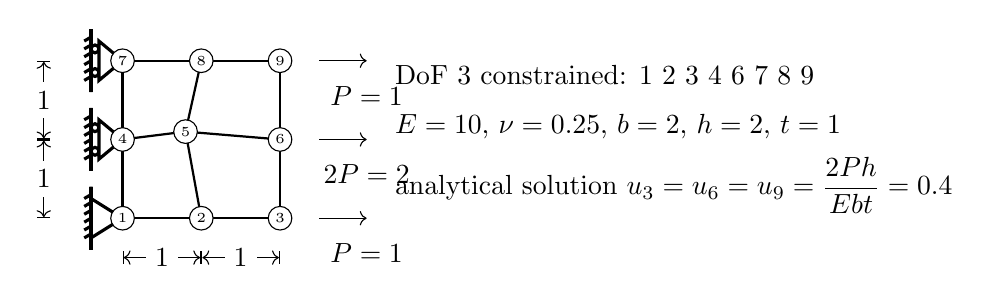
\begin{tikzpicture}[scale=1]
\coordinate(N1)at(0,0);
\coordinate(N2)at(1,0);
\coordinate(N3)at(2,0);
\coordinate(N4)at(0,1);
\coordinate(N5)at(.8,1.1);
\coordinate(N6)at(2,1);
\coordinate(N7)at(0,2);
\coordinate(N8)at(1,2);
\coordinate(N9)at(2,2);
\draw[thick](N1)--(N2)--(N3)--(N6)--(N9)--(N8)--(N7)--(N4)--cycle;
\draw[thick](N2)--(N5)--(N8);
\draw[thick](N4)--(N5)--(N6);
\HingeSupport[-90]{N1};
\RollerSupport[-90]{N4};
\RollerSupport[-90]{N7};
\begin{scope}[every node/.style={fill=white,circle,draw,inner sep=0,minimum size=3mm}]
\node at(N1){\tiny1};
\node at(N2){\tiny2};
\node at(N3){\tiny3};
\node at(N4){\tiny4};
\node at(N5){\tiny5};
\node at(N6){\tiny6};
\node at(N7){\tiny7};
\node at(N8){\tiny8};
\node at(N9){\tiny9};
\end{scope}
\draw[->](2.5,0)--++(.6,0)node[below=2mm]{$P=1$};
\draw[->](2.5,1)--++(.6,0)node[below=2mm]{$2P=2$};
\draw[->](2.5,2)--++(.6,0)node[below=2mm]{$P=1$};
\draw[|<->|](0,-.5)--++(1,0)node[midway,fill=white]{$1$};
\draw[|<->|](1,-.5)--++(1,0)node[midway,fill=white]{$1$};
\draw[|<->|](-1,0)--++(0,1)node[midway,fill=white]{$1$};
\draw[|<->|](-1,1)--++(0,1)node[midway,fill=white]{$1$};
\node[align=left]at(7,1){DoF 3 constrained: 1 2 3 4 6 7 8 9\\[2mm]$E=10$, $\nu=0.25$, $b=2$, $h=2$, $t=1$\\[2mm]analytical solution $u_3=u_6=u_9=\dfrac{2Ph}{Ebt}=0.4$};
\end{tikzpicture}
\caption{constant strain patch test two}\label{fig:gcmq_patch}
\end{figure}
Altering the position of the centre node shows that all three versions of GCMQ could pass the constant strain patch test with arbitrary convex geometries.

\begin{table}[htb]
\centering\scriptsize
\caption{horizontal displacement $u_x$ of the centre node with various coordinates}\label{tab:patch_ii_a}
\begin{tabular}{ccccccc}
	\toprule
	\diagbox{$y$}{$x$} & \num{0.6}\footnote{origin of c.s. is set to node 1} & \num{0.7}  & \num{0.8}  & \num{0.9}  & \num{1.0}  & theoretical \\ \midrule
	    \num{0.6}      &                  \num{0.12}                   & \num{0.12} & \num{0.12} & \num{0.12} & \num{0.12} & \num{0.12}  \\
	    \num{0.7}      &                                               & \num{0.14} & \num{0.14} & \num{0.14} & \num{0.14} & \num{0.14}  \\
	    \num{0.8}      &                                               &            & \num{0.16} & \num{0.16} & \num{0.16} & \num{0.16}  \\
	    \num{0.9}      &                                               &            &            & \num{0.18} & \num{0.18} & \num{0.18}  \\
	    \num{1.0}      &                                               &            &            &            & \num{0.20} & \num{0.20}  \\ \bottomrule
\end{tabular}
\end{table}
Numerical results are shown in \tabref{tab:patch_ii_a}. Clearly, as can be proved by both horizontal and vertical (not shown here for brevity) displacement of the centre node, the linear displacement field is produced by GCMQ. The constant stress field with components $\sigma_x=2$ and $\sigma_y=\tau_{xy}=0$ is also produced in all cases listed.
\subsection{Shear and Volumetric Locking}
\subsubsection{MacNeal's Thin Beam}
The MacNeal's thin beam \citep{MacNeal1985} is used for shear locking test. The geometry is \numproduct{0.2x6} with three different meshes as shown in \figref{example:macneals_beam} where $t$ is beam thickness, $E$ is elastic modulus and $\nu$ is Poisson's ratio. Two loads ($P$ and $M$) are applied at the free end. The unit shear load $P$ is evenly split on two end nodes while the moment load $M$ is applied in the form of concentrated force pair.
\begin{figure}[H]
\centering\scriptsize
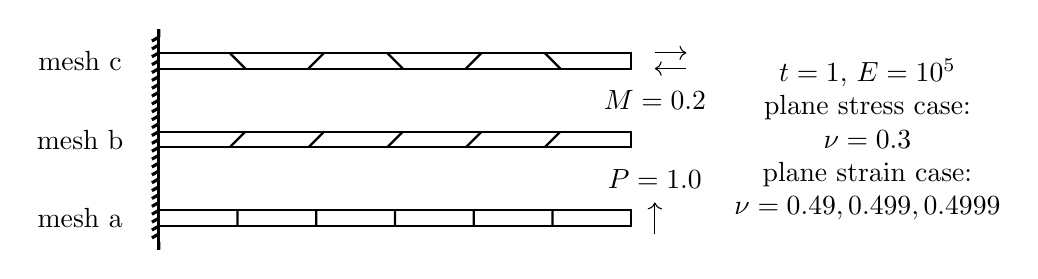
\begin{tikzpicture}
\FixedSupport[-90]{0,1.1}{3.5}
\node at(-1,.1){mesh a};
\node at(-1,1.1){mesh b};
\node at(-1,2.1){mesh c};
\draw[thick](0,0)rectangle(6,.2)(0,1)rectangle(6,1.2)(0,2)rectangle(6,2.2);
\foreach\x in{1,2,3,4,5}\draw[thick](\x,0)--++(0,.2)(\x-.1,1)--++(.2,.2);
\foreach\x in{1,3,5}\draw[thick](\x+.1,2)--++(-.2,.2);
\foreach\x in{2,4}\draw[thick](\x-.1,2)--++(.2,.2);
\draw[->](6.3,-.1)--++(0,.4);
\draw[<-](6.3,2)--++(.4,0);
\draw[->](6.3,2.2)--++(.4,0);
\node at(6.3,1.6){$M=0.2$};
\node at(6.3,.6){$P=1.0$};
\node[align=center]at(9,1.1){$t=1$, $E=\num{E5}$\\plane stress case:\\$\nu=0.3$\\plane strain case:\\$\nu=0.49,0.499,0.4999$};
\end{tikzpicture}
\caption{MacNeal's thin beam}\label{example:macneals_beam}
\end{figure}

The results are shown in \tabref{table:macneals_beam_shear}. The least accurate tip deflection of \num{1.0488} is approximate \SI{97}{\percent} of the reference value. It could be concluded from \tabref{table:macneals_beam_shear} that GCMQ element does not lock subjected to pure end shear and moment. Although there are only four nodes, GCMQ element can properly describe shear response as by construction it supports a non-linear distribution of stress and strain.
\begin{table}[H]
\centering\scriptsize
\caption{tip deflections of plane stress MacNeal's thin beam}\label{table:macneals_beam_shear}
\begin{tabular}{lcccccc}
	\toprule
	                      & \multicolumn{3}{c}{$P$}  & \multicolumn{3}{c}{$M$}  \\
	                      & mesh a & mesh b & mesh c & mesh a & mesh b & mesh c \\ \midrule
	GCMQ-I                & 1.0733 & 1.0488 & 1.0654 & 0.0540 & 0.0538 & 0.0537 \\
	GCMQ-L                & 1.0733 & 1.0464 & 1.0665 & 0.0540 & 0.0537 & 0.0539 \\
	GCMQ-G                & 1.0733 & 1.0467 & 1.0638 & 0.0540 & 0.0536 & 0.0538 \\ \midrule
	ref. \citep{Cen2015} & 1.0812 &        &        & 0.0540 &        &        \\ \bottomrule
\end{tabular}
\end{table}

The same beam can also be used for volumetric locking test. Accordingly, three Poisson's ratios close to incompressibility $\nu=0.5$ are chosen. The results in \tabref{table:macneals_beam_volumetric} show no sensitivity to (near) incompressibility problems. The worst results, which occur with Irons schemes and parallelogram meshes subjected to end shear, are about the same level (\SI{96.7}{\percent} of the reference values) for all Poisson's ratios. The overall performance of GCMQ is slightly better than recent elements. Comparisons are available elsewhere \citep{Cen2015} thus not shown here for brevity.
\begin{table}[H]
\centering\scriptsize
\caption{tip deflections of plane strain MacNeal's thin beam}\label{table:macneals_beam_volumetric}
\begin{tabular}{lcccccc}
	\toprule
	                     & \multicolumn{3}{c}{$P$}  & \multicolumn{3}{c}{$M$}  \\
	                     & mesh a & mesh b & mesh c & mesh a & mesh b & mesh c \\ \midrule
	                     &           \multicolumn{6}{c}{$\nu=0.49$}            \\
	GCMQ-I               & 0.8159 & 0.7947 & 0.8078 & 0.0410 & 0.0408 & 0.0408 \\
	GCMQ-L               & 0.8159 & 0.7956 & 0.8103 & 0.0410 & 0.0409 & 0.0409 \\
	GCMQ-G               & 0.8159 & 0.7966 & 0.8102 & 0.0410 & 0.0409 & 0.0409 \\
	ref.                 & 0.8217 &        &        & 0.0410 &        &        \\ \midrule
	                     &           \multicolumn{6}{c}{$\nu=0.499$}           \\
	GCMQ-I               & 0.8063 & 0.7849 & 0.7978 & 0.0406 & 0.0403 & 0.0403 \\
	GCMQ-L               & 0.8063 & 0.7861 & 0.8007 & 0.0406 & 0.0404 & 0.0404 \\
	GCMQ-G               & 0.8063 & 0.7872 & 0.8007 & 0.0406 & 0.0404 & 0.0404 \\
	ref.                 & 0.8121 &        &        & 0.0406 &        &        \\ \midrule
	                     &          \multicolumn{6}{c}{$\nu=0.4999$}           \\
	GCMQ-I               & 0.8054 & 0.7839 & 0.7968 & 0.0405 & 0.0402 & 0.0402 \\
	GCMQ-L               & 0.8054 & 0.7852 & 0.7998 & 0.0405 & 0.0404 & 0.0404 \\
	GCMQ-G               & 0.8054 & 0.7862 & 0.7997 & 0.0405 & 0.0403 & 0.0404 \\
	ref. \citep{Cen2015} & 0.8111 &        &        & 0.0405 &        &        \\ \bottomrule
\end{tabular}
\end{table} 
\subsubsection{Thick-Walled Cylinder}
A thick-walled cylinder was first proposed by \citet{MacNeal1985} for testing the sensitivity to volumetric locking of new elements. The model and the corresponding mesh grid used are shown in \figref{fig:cylinder}.
\begin{figure}[htb]
\centering\footnotesize
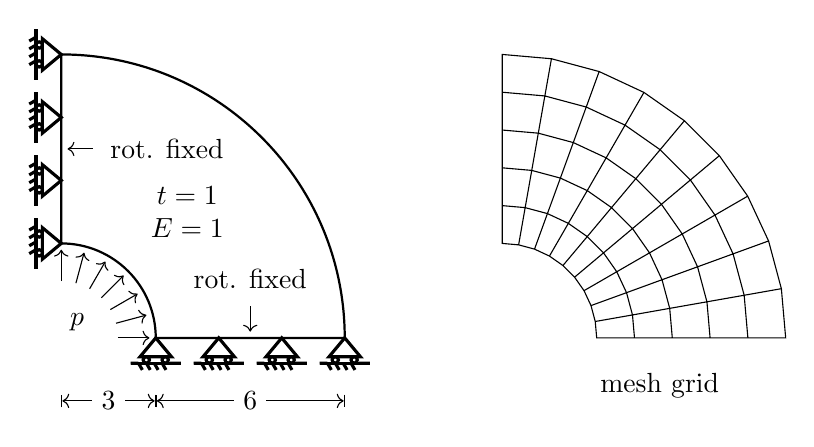
\begin{tikzpicture}[scale=.4]
\RollerSupport{3,0}{2}
\RollerSupport{5,0}{2}
\RollerSupport{7,0}{2}
\RollerSupport{9,0}{2}
\RollerSupport[-90]{0,3}{2}
\RollerSupport[-90]{0,5}{2}
\RollerSupport[-90]{0,7}{2}
\RollerSupport[-90]{0,9}{2}
\foreach\x in {0,15,30,...,90}{\draw[->](\x:1.8)--(\x:2.8);}
\draw[thick](3,0)arc(0:90:3)--++(0,6)arc(90:0:9)--cycle;
\draw[|<->|](0,-2)--++(3,0)node[midway,fill=white]{$3$};
\draw[|<->|](3,-2)--++(6,0)node[midway,fill=white]{$6$};
\node[align=center]at(4,4){$t=1$\\$E=1$};
\node at(.5,.5){$p$};
\draw[<-](.2,6)--(1,6)node[right=1mm]{rot. fixed};
\draw[<-](6,.2)--(6,1)node[above=1mm]{rot. fixed};
\begin{scope}[xshift=140mm]
\node at(5,-1.5){mesh grid};
\coordinate(N1)at(3.000,0.000);
\coordinate(N2)at(4.200,0.000);
\coordinate(N3)at(5.400,0.000);
\coordinate(N4)at(6.600,0.000);
\coordinate(N5)at(7.800,0.000);
\coordinate(N6)at(9.000,0.000);
\coordinate(N7)at(2.954,0.521);
\coordinate(N8)at(4.136,0.729);
\coordinate(N9)at(5.318,0.938);
\coordinate(N10)at(6.500,1.146);
\coordinate(N11)at(7.682,1.354);
\coordinate(N12)at(8.863,1.563);
\coordinate(N13)at(2.819,1.026);
\coordinate(N14)at(3.947,1.436);
\coordinate(N15)at(5.074,1.847);
\coordinate(N16)at(6.202,2.257);
\coordinate(N17)at(7.330,2.668);
\coordinate(N18)at(8.457,3.078);
\coordinate(N19)at(2.598,1.500);
\coordinate(N20)at(3.637,2.100);
\coordinate(N21)at(4.677,2.700);
\coordinate(N22)at(5.716,3.300);
\coordinate(N23)at(6.755,3.900);
\coordinate(N24)at(7.794,4.500);
\coordinate(N25)at(2.298,1.928);
\coordinate(N26)at(3.217,2.700);
\coordinate(N27)at(4.137,3.471);
\coordinate(N28)at(5.056,4.242);
\coordinate(N29)at(5.975,5.014);
\coordinate(N30)at(6.894,5.785);
\coordinate(N31)at(1.928,2.298);
\coordinate(N32)at(2.700,3.217);
\coordinate(N33)at(3.471,4.137);
\coordinate(N34)at(4.242,5.056);
\coordinate(N35)at(5.014,5.975);
\coordinate(N36)at(5.785,6.894);
\coordinate(N37)at(1.500,2.598);
\coordinate(N38)at(2.100,3.637);
\coordinate(N39)at(2.700,4.677);
\coordinate(N40)at(3.300,5.716);
\coordinate(N41)at(3.900,6.755);
\coordinate(N42)at(4.500,7.794);
\coordinate(N43)at(1.026,2.819);
\coordinate(N44)at(1.436,3.947);
\coordinate(N45)at(1.847,5.074);
\coordinate(N46)at(2.257,6.202);
\coordinate(N47)at(2.668,7.330);
\coordinate(N48)at(3.078,8.457);
\coordinate(N49)at(0.521,2.954);
\coordinate(N50)at(0.729,4.136);
\coordinate(N51)at(0.938,5.318);
\coordinate(N52)at(1.146,6.500);
\coordinate(N53)at(1.354,7.682);
\coordinate(N54)at(1.563,8.863);
\coordinate(N55)at(0.000,3.000);
\coordinate(N56)at(0.000,4.200);
\coordinate(N57)at(0.000,5.400);
\coordinate(N58)at(0.000,6.600);
\coordinate(N59)at(0.000,7.800);
\coordinate(N60)at(0.000,9.000);
\draw
(N1)--(N2)--(N8)--(N7)--cycle
(N2)--(N3)--(N9)--(N8)--cycle
(N3)--(N4)--(N10)--(N9)--cycle
(N4)--(N5)--(N11)--(N10)--cycle
(N5)--(N6)--(N12)--(N11)--cycle
(N7)--(N8)--(N14)--(N13)--cycle
(N8)--(N9)--(N15)--(N14)--cycle
(N9)--(N10)--(N16)--(N15)--cycle
(N10)--(N11)--(N17)--(N16)--cycle
(N11)--(N12)--(N18)--(N17)--cycle
(N13)--(N14)--(N20)--(N19)--cycle
(N14)--(N15)--(N21)--(N20)--cycle
(N15)--(N16)--(N22)--(N21)--cycle
(N16)--(N17)--(N23)--(N22)--cycle
(N17)--(N18)--(N24)--(N23)--cycle
(N19)--(N20)--(N26)--(N25)--cycle
(N20)--(N21)--(N27)--(N26)--cycle
(N21)--(N22)--(N28)--(N27)--cycle
(N22)--(N23)--(N29)--(N28)--cycle
(N23)--(N24)--(N30)--(N29)--cycle
(N25)--(N26)--(N32)--(N31)--cycle
(N26)--(N27)--(N33)--(N32)--cycle
(N27)--(N28)--(N34)--(N33)--cycle
(N28)--(N29)--(N35)--(N34)--cycle
(N29)--(N30)--(N36)--(N35)--cycle
(N31)--(N32)--(N38)--(N37)--cycle
(N32)--(N33)--(N39)--(N38)--cycle
(N33)--(N34)--(N40)--(N39)--cycle
(N34)--(N35)--(N41)--(N40)--cycle
(N35)--(N36)--(N42)--(N41)--cycle
(N37)--(N38)--(N44)--(N43)--cycle
(N38)--(N39)--(N45)--(N44)--cycle
(N39)--(N40)--(N46)--(N45)--cycle
(N40)--(N41)--(N47)--(N46)--cycle
(N41)--(N42)--(N48)--(N47)--cycle
(N43)--(N44)--(N50)--(N49)--cycle
(N44)--(N45)--(N51)--(N50)--cycle
(N45)--(N46)--(N52)--(N51)--cycle
(N46)--(N47)--(N53)--(N52)--cycle
(N47)--(N48)--(N54)--(N53)--cycle
(N49)--(N50)--(N56)--(N55)--cycle
(N50)--(N51)--(N57)--(N56)--cycle
(N51)--(N52)--(N58)--(N57)--cycle
(N52)--(N53)--(N59)--(N58)--cycle
(N53)--(N54)--(N60)--(N59)--cycle;
\end{scope}
\end{tikzpicture}
\caption{thick-walled cylinder subjected to unit pressure}\label{fig:cylinder}
\end{figure}
The analytical solution of radial displacement is given by
\begin{gather}
u=\dfrac{\left(1+\nu\right)pR_1^2}{E\left(R_2^2-R_1^2\right)}\left(\dfrac{R_2^2}{r}+\left(1-2\nu\right)r\right),
\end{gather}
where $p$ is the pressure, $R_1$ is the inner radius and $R_2$ is the outer radius. For $r=R_1$,
\begin{gather}
u=\dfrac{3}{4}\left(1+\nu\right)\left(5-\nu\right),
\end{gather}

Numerical results with different Poisson's ratios are shown in \tabref{tab:cylinder}. No volumetric locking is observed as the error stays around the same level (\SI{3}{\percent}) for all valid Poisson's ratios. The numerical failure is caused due to ill-conditioned stiffness matrix, rather than the element formulation. In fact, GCMQ accepts completely incompressible material, viz., $\nu=0.5$, in which case, the corresponding $\mb{C}$ matrix is well-conditioned.
\begin{table}[htb]
\centering\footnotesize
\caption{radial displacement at inner radius of thick-walled cylinder}\label{tab:cylinder}
\begin{tabular}{lrrrrrrr}
	\toprule
	$\nu$      &   0.49 &  0.499 & 0.4999 & 0.49999 & 0.499999 & 0.4999999 & 0.49999999 \\ \midrule
	GCMQ-I     & 4.8888 & 4.8988 & 4.8997 &  4.8997 &   4.8998 &    4.8998 &     4.8998 \\
	GCMQ-L     & 4.8850 & 4.8942 & 4.8950 &  4.8951 &   4.8951 &    4.8951 &     4.8951 \\
	GCMQ-G     & 4.8852 & 4.8941 & 4.8949 &  4.8950 &   4.8950 &    4.8950 &     4.8950 \\
	analytical & 5.0399 & 5.0602 & 5.0623 &  5.0625 &   5.0625 &    5.0625 &     5.0625 \\ \bottomrule
\end{tabular}
\end{table}
\subsubsection{Mesh Distortion}
Mesh distortion is undesirable in general but cannot be avoided, especially for complex geometries. A simple cantilever beam with two elements defined is used to benchmark the sensitivity to mesh distortion. The model is shown in \figref{fig:distortion}.
\begin{figure}[htb]
\centering\footnotesize
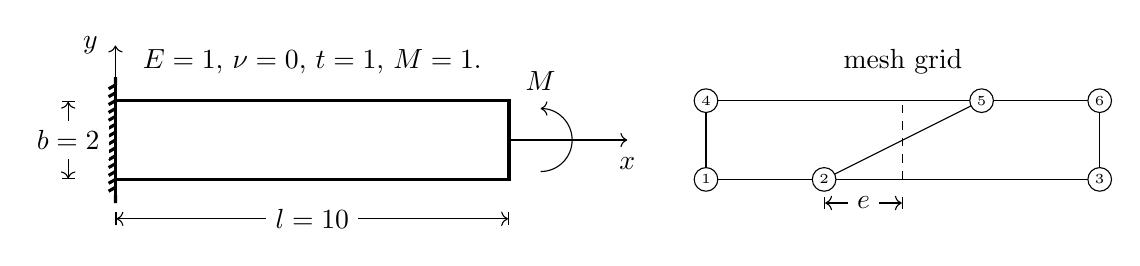
\begin{tikzpicture}
\def\a{1}\def\b{.5}
\FixedSupport[-90]{0,0}{2}
\draw[->](0,0)--(0,\a+.2)node[left=1mm]{$y$};
\draw[->](0,0)--(10*\b+1.5,0)node[below=1mm]{$x$};
\draw[very thick,fill=white](0,-\b)rectangle(10*\b,\b);
\draw[|<->|](-.6,\b)--++(0,-2*\b)node[fill=white,midway]{$b=2$};
\draw[|<->|](0,-\b-.5)--++(10*\b,0)node[fill=white,midway]{$l=10$};
\draw[->](10*\b+.4,-.4)arc(-90:90:.4)node[above=1mm]{$M$};
\node[align=center]at(5*\b,\b+.5){$E=1$, $\nu=0$, $t=1$, $M=1$.};
\begin{scope}[xshift=75mm]
\node[align=center]at(5*\b,\b+.5){mesh grid};
\draw(0,-\b)rectangle(10*\b,\b);
\draw[dashed](5*\b,-\b)--++(0,2*\b);
\draw(3*\b,-\b)--(7*\b,\b);
\draw[|<->|](3*\b,-\b-.3)--(5*\b,-\b-.3)node[fill=white,midway]{$e$};
\begin{scope}[every node/.style={fill=white,circle,draw,inner sep=0,minimum size=3mm}]
\node at(0,-\b){\tiny1};
\node at(3*\b,-\b){\tiny2};
\node at(10*\b,-\b){\tiny3};
\node at(0,\b){\tiny4};
\node at(7*\b,\b){\tiny5};
\node at(10*\b,\b){\tiny6};
\end{scope}
\end{scope}
\end{tikzpicture}
\caption{cantilever beam with mesh distortion}\label{fig:distortion}
\end{figure}

To exactly model the fixed boundary condition, a trivial Poisson's ratio is used. For pure bending, the analytical solution of tip deflection \citep{Timoshenko1970} can be obtained as
\begin{gather}
v=\dfrac{Ml^2}{2EI}=\dfrac{1\times10^2\times6}{1\times1\times2^3}=75,
\end{gather}
which is identical to the solution given by the simple bending theory in mechanics of materials. Similar to previous examples, the moment $M$ can be applied as either force pair or conjugate moment, which is the corresponding force component on the drilling DoF. The parameter $e$ controls the degree of distortion and ranges from \num{-5} to \num{5}. Varying it gives the following results as shown in \figref{fig:distortion_result}.
\begin{figure}[htb]
\centering\scriptsize
\begin{subfigure}[b]{.49\textwidth}\centering
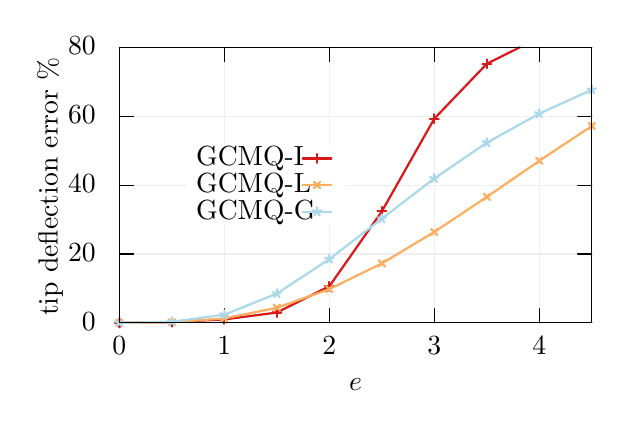
\begin{tikzpicture}[gnuplot]
%% generated with GNUPLOT 5.2p6 (Lua 5.3; terminal rev. Nov 2018, script rev. 107)
%% 02/27/2019 02:19:29
\path (0.000,0.000) rectangle (6.000,3.500);
\gpcolor{rgb color={0.933,0.933,0.933}}
\gpsetlinetype{gp lt border}
\gpsetdashtype{gp dt solid}
\gpsetlinewidth{1.00}
\draw[gp path] (0.000,0.000)--(5.999,0.000);
\gpcolor{color=gp lt color border}
\draw[gp path] (0.000,0.000)--(0.180,0.000);
\draw[gp path] (5.999,0.000)--(5.819,0.000);
\node[gp node right] at (-0.184,0.000) {$0$};
\gpcolor{rgb color={0.933,0.933,0.933}}
\draw[gp path] (0.000,0.875)--(5.999,0.875);
\gpcolor{color=gp lt color border}
\draw[gp path] (0.000,0.875)--(0.180,0.875);
\draw[gp path] (5.999,0.875)--(5.819,0.875);
\node[gp node right] at (-0.184,0.875) {$20$};
\gpcolor{rgb color={0.933,0.933,0.933}}
\draw[gp path] (0.000,1.750)--(0.856,1.750);
\draw[gp path] (2.876,1.750)--(5.999,1.750);
\gpcolor{color=gp lt color border}
\draw[gp path] (0.000,1.750)--(0.180,1.750);
\draw[gp path] (5.999,1.750)--(5.819,1.750);
\node[gp node right] at (-0.184,1.750) {$40$};
\gpcolor{rgb color={0.933,0.933,0.933}}
\draw[gp path] (0.000,2.624)--(5.999,2.624);
\gpcolor{color=gp lt color border}
\draw[gp path] (0.000,2.624)--(0.180,2.624);
\draw[gp path] (5.999,2.624)--(5.819,2.624);
\node[gp node right] at (-0.184,2.624) {$60$};
\gpcolor{rgb color={0.933,0.933,0.933}}
\draw[gp path] (0.000,3.499)--(5.999,3.499);
\gpcolor{color=gp lt color border}
\draw[gp path] (0.000,3.499)--(0.180,3.499);
\draw[gp path] (5.999,3.499)--(5.819,3.499);
\node[gp node right] at (-0.184,3.499) {$80$};
\gpcolor{rgb color={0.933,0.933,0.933}}
\draw[gp path] (0.000,0.000)--(0.000,3.499);
\gpcolor{color=gp lt color border}
\draw[gp path] (0.000,0.000)--(0.000,0.180);
\draw[gp path] (0.000,3.499)--(0.000,3.319);
\node[gp node center] at (0.000,-0.308) {$0$};
\gpcolor{rgb color={0.933,0.933,0.933}}
\draw[gp path] (1.333,0.000)--(1.333,1.243);
\draw[gp path] (1.333,2.257)--(1.333,3.499);
\gpcolor{color=gp lt color border}
\draw[gp path] (1.333,0.000)--(1.333,0.180);
\draw[gp path] (1.333,3.499)--(1.333,3.319);
\node[gp node center] at (1.333,-0.308) {$1$};
\gpcolor{rgb color={0.933,0.933,0.933}}
\draw[gp path] (2.666,0.000)--(2.666,1.243);
\draw[gp path] (2.666,2.257)--(2.666,3.499);
\gpcolor{color=gp lt color border}
\draw[gp path] (2.666,0.000)--(2.666,0.180);
\draw[gp path] (2.666,3.499)--(2.666,3.319);
\node[gp node center] at (2.666,-0.308) {$2$};
\gpcolor{rgb color={0.933,0.933,0.933}}
\draw[gp path] (3.999,0.000)--(3.999,3.499);
\gpcolor{color=gp lt color border}
\draw[gp path] (3.999,0.000)--(3.999,0.180);
\draw[gp path] (3.999,3.499)--(3.999,3.319);
\node[gp node center] at (3.999,-0.308) {$3$};
\gpcolor{rgb color={0.933,0.933,0.933}}
\draw[gp path] (5.332,0.000)--(5.332,3.499);
\gpcolor{color=gp lt color border}
\draw[gp path] (5.332,0.000)--(5.332,0.180);
\draw[gp path] (5.332,3.499)--(5.332,3.319);
\node[gp node center] at (5.332,-0.308) {$4$};
\draw[gp path] (0.000,3.499)--(0.000,0.000)--(5.999,0.000)--(5.999,3.499)--cycle;
\node[gp node center,rotate=-270] at (-0.860,1.749) {tip deflection error \si{\percent}};
\node[gp node center] at (2.999,-0.769) {$e$};
\node[gp node left] at (0.856,2.088) {GCMQ-I};
\gpcolor{rgb color={0.843,0.098,0.110}}
\gpsetlinewidth{2.00}
\draw[gp path] (2.328,2.088)--(2.692,2.088);
\draw[gp path] (0.000,0.000)--(0.667,0.010)--(1.333,0.044)--(2.000,0.131)--(2.666,0.464)%
  --(3.333,1.416)--(3.999,2.593)--(4.666,3.290)--(5.085,3.499);
\gpsetpointsize{4.00}
\gppoint{gp mark 1}{(0.000,0.000)}
\gppoint{gp mark 1}{(0.667,0.010)}
\gppoint{gp mark 1}{(1.333,0.044)}
\gppoint{gp mark 1}{(2.000,0.131)}
\gppoint{gp mark 1}{(2.666,0.464)}
\gppoint{gp mark 1}{(3.333,1.416)}
\gppoint{gp mark 1}{(3.999,2.593)}
\gppoint{gp mark 1}{(4.666,3.290)}
\gppoint{gp mark 1}{(2.510,2.088)}
\gpcolor{color=gp lt color border}
\node[gp node left] at (0.856,1.750) {GCMQ-L};
\gpcolor{rgb color={0.992,0.682,0.380}}
\draw[gp path] (2.328,1.750)--(2.692,1.750);
\draw[gp path] (0.000,0.000)--(0.667,0.008)--(1.333,0.056)--(2.000,0.191)--(2.666,0.428)%
  --(3.333,0.755)--(3.999,1.154)--(4.666,1.599)--(5.332,2.058)--(5.999,2.500);
\gppoint{gp mark 2}{(0.000,0.000)}
\gppoint{gp mark 2}{(0.667,0.008)}
\gppoint{gp mark 2}{(1.333,0.056)}
\gppoint{gp mark 2}{(2.000,0.191)}
\gppoint{gp mark 2}{(2.666,0.428)}
\gppoint{gp mark 2}{(3.333,0.755)}
\gppoint{gp mark 2}{(3.999,1.154)}
\gppoint{gp mark 2}{(4.666,1.599)}
\gppoint{gp mark 2}{(5.332,2.058)}
\gppoint{gp mark 2}{(5.999,2.500)}
\gppoint{gp mark 2}{(2.510,1.750)}
\gpcolor{color=gp lt color border}
\node[gp node left] at (0.856,1.412) {GCMQ-G};
\gpcolor{rgb color={0.671,0.851,0.914}}
\draw[gp path] (2.328,1.412)--(2.692,1.412);
\draw[gp path] (0.000,0.000)--(0.667,0.014)--(1.333,0.104)--(2.000,0.372)--(2.666,0.809)%
  --(3.333,1.323)--(3.999,1.834)--(4.666,2.288)--(5.332,2.657)--(5.999,2.960);
\gppoint{gp mark 3}{(0.000,0.000)}
\gppoint{gp mark 3}{(0.667,0.014)}
\gppoint{gp mark 3}{(1.333,0.104)}
\gppoint{gp mark 3}{(2.000,0.372)}
\gppoint{gp mark 3}{(2.666,0.809)}
\gppoint{gp mark 3}{(3.333,1.323)}
\gppoint{gp mark 3}{(3.999,1.834)}
\gppoint{gp mark 3}{(4.666,2.288)}
\gppoint{gp mark 3}{(5.332,2.657)}
\gppoint{gp mark 3}{(5.999,2.960)}
\gppoint{gp mark 3}{(2.510,1.412)}
\gpcolor{color=gp lt color border}
\gpsetlinewidth{1.00}
\draw[gp path] (0.000,3.499)--(0.000,0.000)--(5.999,0.000)--(5.999,3.499)--cycle;
%% coordinates of the plot area
\gpdefrectangularnode{gp plot 1}{\pgfpoint{0.000cm}{0.000cm}}{\pgfpoint{5.999cm}{3.499cm}}
\end{tikzpicture}
%% gnuplot variables

\caption{load applied as force pair}
\end{subfigure}\quad
\begin{subfigure}[b]{.49\textwidth}\centering
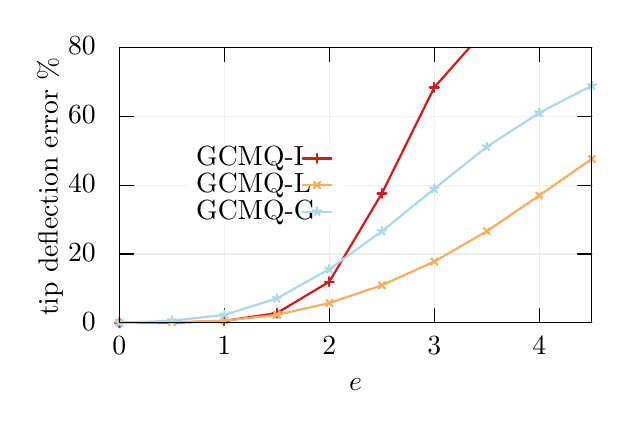
\begin{tikzpicture}[gnuplot]
%% generated with GNUPLOT 5.2p6 (Lua 5.3; terminal rev. Nov 2018, script rev. 107)
%% 02/27/2019 02:19:31
\path (0.000,0.000) rectangle (6.000,3.500);
\gpcolor{rgb color={0.933,0.933,0.933}}
\gpsetlinetype{gp lt border}
\gpsetdashtype{gp dt solid}
\gpsetlinewidth{1.00}
\draw[gp path] (0.000,0.000)--(5.999,0.000);
\gpcolor{color=gp lt color border}
\draw[gp path] (0.000,0.000)--(0.180,0.000);
\draw[gp path] (5.999,0.000)--(5.819,0.000);
\node[gp node right] at (-0.184,0.000) {$0$};
\gpcolor{rgb color={0.933,0.933,0.933}}
\draw[gp path] (0.000,0.875)--(5.999,0.875);
\gpcolor{color=gp lt color border}
\draw[gp path] (0.000,0.875)--(0.180,0.875);
\draw[gp path] (5.999,0.875)--(5.819,0.875);
\node[gp node right] at (-0.184,0.875) {$20$};
\gpcolor{rgb color={0.933,0.933,0.933}}
\draw[gp path] (0.000,1.750)--(0.856,1.750);
\draw[gp path] (2.876,1.750)--(5.999,1.750);
\gpcolor{color=gp lt color border}
\draw[gp path] (0.000,1.750)--(0.180,1.750);
\draw[gp path] (5.999,1.750)--(5.819,1.750);
\node[gp node right] at (-0.184,1.750) {$40$};
\gpcolor{rgb color={0.933,0.933,0.933}}
\draw[gp path] (0.000,2.624)--(5.999,2.624);
\gpcolor{color=gp lt color border}
\draw[gp path] (0.000,2.624)--(0.180,2.624);
\draw[gp path] (5.999,2.624)--(5.819,2.624);
\node[gp node right] at (-0.184,2.624) {$60$};
\gpcolor{rgb color={0.933,0.933,0.933}}
\draw[gp path] (0.000,3.499)--(5.999,3.499);
\gpcolor{color=gp lt color border}
\draw[gp path] (0.000,3.499)--(0.180,3.499);
\draw[gp path] (5.999,3.499)--(5.819,3.499);
\node[gp node right] at (-0.184,3.499) {$80$};
\gpcolor{rgb color={0.933,0.933,0.933}}
\draw[gp path] (0.000,0.000)--(0.000,3.499);
\gpcolor{color=gp lt color border}
\draw[gp path] (0.000,0.000)--(0.000,0.180);
\draw[gp path] (0.000,3.499)--(0.000,3.319);
\node[gp node center] at (0.000,-0.308) {$0$};
\gpcolor{rgb color={0.933,0.933,0.933}}
\draw[gp path] (1.333,0.000)--(1.333,1.243);
\draw[gp path] (1.333,2.257)--(1.333,3.499);
\gpcolor{color=gp lt color border}
\draw[gp path] (1.333,0.000)--(1.333,0.180);
\draw[gp path] (1.333,3.499)--(1.333,3.319);
\node[gp node center] at (1.333,-0.308) {$1$};
\gpcolor{rgb color={0.933,0.933,0.933}}
\draw[gp path] (2.666,0.000)--(2.666,1.243);
\draw[gp path] (2.666,2.257)--(2.666,3.499);
\gpcolor{color=gp lt color border}
\draw[gp path] (2.666,0.000)--(2.666,0.180);
\draw[gp path] (2.666,3.499)--(2.666,3.319);
\node[gp node center] at (2.666,-0.308) {$2$};
\gpcolor{rgb color={0.933,0.933,0.933}}
\draw[gp path] (3.999,0.000)--(3.999,3.499);
\gpcolor{color=gp lt color border}
\draw[gp path] (3.999,0.000)--(3.999,0.180);
\draw[gp path] (3.999,3.499)--(3.999,3.319);
\node[gp node center] at (3.999,-0.308) {$3$};
\gpcolor{rgb color={0.933,0.933,0.933}}
\draw[gp path] (5.332,0.000)--(5.332,3.499);
\gpcolor{color=gp lt color border}
\draw[gp path] (5.332,0.000)--(5.332,0.180);
\draw[gp path] (5.332,3.499)--(5.332,3.319);
\node[gp node center] at (5.332,-0.308) {$4$};
\draw[gp path] (0.000,3.499)--(0.000,0.000)--(5.999,0.000)--(5.999,3.499)--cycle;
\node[gp node center,rotate=-270] at (-0.860,1.749) {tip deflection error \si{\percent}};
\node[gp node center] at (2.999,-0.769) {$e$};
\node[gp node left] at (0.856,2.088) {GCMQ-I};
\gpcolor{rgb color={0.843,0.098,0.110}}
\gpsetlinewidth{2.00}
\draw[gp path] (2.328,2.088)--(2.692,2.088);
\draw[gp path] (0.000,0.000)--(0.667,0.000)--(1.333,0.025)--(2.000,0.124)--(2.666,0.523)%
  --(3.333,1.643)--(3.999,2.990)--(4.449,3.499);
\gpsetpointsize{4.00}
\gppoint{gp mark 1}{(0.000,0.000)}
\gppoint{gp mark 1}{(1.333,0.025)}
\gppoint{gp mark 1}{(2.000,0.124)}
\gppoint{gp mark 1}{(2.666,0.523)}
\gppoint{gp mark 1}{(3.333,1.643)}
\gppoint{gp mark 1}{(3.999,2.990)}
\gppoint{gp mark 1}{(2.510,2.088)}
\gpcolor{color=gp lt color border}
\node[gp node left] at (0.856,1.750) {GCMQ-L};
\gpcolor{rgb color={0.992,0.682,0.380}}
\draw[gp path] (2.328,1.750)--(2.692,1.750);
\draw[gp path] (0.000,0.000)--(0.667,0.008)--(1.333,0.027)--(2.000,0.101)--(2.666,0.252)%
  --(3.333,0.477)--(3.999,0.778)--(4.666,1.164)--(5.332,1.617)--(5.999,2.082);
\gppoint{gp mark 2}{(0.000,0.000)}
\gppoint{gp mark 2}{(0.667,0.008)}
\gppoint{gp mark 2}{(1.333,0.027)}
\gppoint{gp mark 2}{(2.000,0.101)}
\gppoint{gp mark 2}{(2.666,0.252)}
\gppoint{gp mark 2}{(3.333,0.477)}
\gppoint{gp mark 2}{(3.999,0.778)}
\gppoint{gp mark 2}{(4.666,1.164)}
\gppoint{gp mark 2}{(5.332,1.617)}
\gppoint{gp mark 2}{(5.999,2.082)}
\gppoint{gp mark 2}{(2.510,1.750)}
\gpcolor{color=gp lt color border}
\node[gp node left] at (0.856,1.412) {GCMQ-G};
\gpcolor{rgb color={0.671,0.851,0.914}}
\draw[gp path] (2.328,1.412)--(2.692,1.412);
\draw[gp path] (0.000,0.000)--(0.667,0.027)--(1.333,0.101)--(2.000,0.310)--(2.666,0.683)%
  --(3.333,1.163)--(3.999,1.703)--(4.666,2.236)--(5.332,2.667)--(5.999,3.012);
\gppoint{gp mark 3}{(0.000,0.000)}
\gppoint{gp mark 3}{(0.667,0.027)}
\gppoint{gp mark 3}{(1.333,0.101)}
\gppoint{gp mark 3}{(2.000,0.310)}
\gppoint{gp mark 3}{(2.666,0.683)}
\gppoint{gp mark 3}{(3.333,1.163)}
\gppoint{gp mark 3}{(3.999,1.703)}
\gppoint{gp mark 3}{(4.666,2.236)}
\gppoint{gp mark 3}{(5.332,2.667)}
\gppoint{gp mark 3}{(5.999,3.012)}
\gppoint{gp mark 3}{(2.510,1.412)}
\gpcolor{color=gp lt color border}
\gpsetlinewidth{1.00}
\draw[gp path] (0.000,3.499)--(0.000,0.000)--(5.999,0.000)--(5.999,3.499)--cycle;
%% coordinates of the plot area
\gpdefrectangularnode{gp plot 1}{\pgfpoint{0.000cm}{0.000cm}}{\pgfpoint{5.999cm}{3.499cm}}
\end{tikzpicture}
%% gnuplot variables

\caption{load applied as moment}
\end{subfigure}
\caption{averaged tip deflection error in the mesh distortion test}\label{fig:distortion_result}
\end{figure}
Clearly, GCMQ is not fully insensitive to mesh distortion. However, compared to other elements \citep[cf.][]{Cen2015}, the overall accuracy of GCMQ is good, especially with a Lobatto integration scheme. For all three versions, when $\left\lvert{}e\right\rvert\leqslant1$, viz., the smallest internal angle is greater than \SI{45}{\degree}, slight accuracy degradation is observed which indicates GCMQ is almost insensitive to mesh distortion with similar mesh configurations. Such a threshold can be relaxed to even $\left\lvert{}e\right\rvert\leqslant2$, which corresponds to a rarely seen element geometry in real life simulations. Practically, as long as the mesh grid is not extremely distorted, sensitivity to mesh distortion is in general not a problem.

Isoparametric mapping is known to be one of the reasons that cause sensitivity to mesh distortion \citep{Lee1993}. The recent approach to address this problem is the area coordinate method \citep{Long2010}. However, the resulting elements cannot pass the $C^0$ patch test. Some asymmetric elements \cite[e.g.,][]{Cen2015} can also address this problem, but their asymmetric feature may be undesired in some cases.
\subsection{Overall Accuracy}
\subsubsection{Cantilever Beam with Irregular Mesh}
This example uses the sample beam from the previous example but with a different mesh configuration that is depicted in \figref{example:cantilever_beam}. Shear load $P$ and bending load $M$ are applied separately.
\begin{figure}[H]
\centering\scriptsize
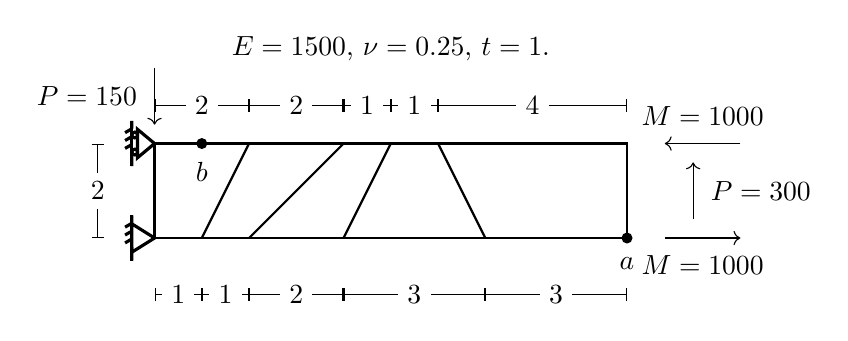
\begin{tikzpicture}[scale=1.2]
\draw[thick](0,0)rectangle(5,1);
\draw[thick](.5,0)--(1,1)(1,0)--(2,1)(2,0)--(2.5,1)(3.5,0)--(3,1);
\draw[|-|](-.6,0)--(-.6,1)node[midway,fill=white]{$2$};
\draw[|-|](0,-.6)--(.5,-.6)node[midway,fill=white]{$1$};
\draw[|-|](.5,-.6)--(1,-.6)node[midway,fill=white]{$1$};
\draw[|-|](1,-.6)--(2,-.6)node[midway,fill=white]{$2$};
\draw[|-|](2,-.6)--(3.5,-.6)node[midway,fill=white]{$3$};
\draw[|-|](3.5,-.6)--(5,-.6)node[midway,fill=white]{$3$};
\draw[|-|](0,1.4)--(1,1.4)node[midway,fill=white]{$2$};
\draw[|-|](1,1.4)--(2,1.4)node[midway,fill=white]{$2$};
\draw[|-|](2,1.4)--(2.5,1.4)node[midway,fill=white]{$1$};
\draw[|-|](2.5,1.4)--(3,1.4)node[midway,fill=white]{$1$};
\draw[|-|](3,1.4)--(5,1.4)node[midway,fill=white]{$4$};
\node[align=center]at(2.5,2){$E=1500$, $\nu=0.25$, $t=1$.};
\node[circle,fill=black,inner sep=0,minimum size=1.4mm]at(5,0){};
\node[anchor=north]at(5,-.1){$a$};
\node[circle,fill=black,inner sep=0,minimum size=1.4mm]at(.5,1){};
\node[anchor=north]at(.5,.9){$b$};
\HingeSupport[-90]{0,0}{.6}
\RollerSupport[-90]{0,1}{.6}
\draw[->](5.7,.2)--++(0,.6)node[midway,right=1mm]{$P=300$};
\draw[->](0,1.8)--++(0,-.6)node[midway,left=1mm]{$P=150$};
\draw[->](5.4,0)--++(.8,0)node[midway,below=1mm]{$M=1000$};
\draw[->](6.2,1)--++(-.8,0)node[midway,above=1mm]{$M=1000$};
\end{tikzpicture}
\caption{cantilever beam with irregular mesh}\label{example:cantilever_beam}
\end{figure}

The overall accuracy of both displacement and stress results are good, as can be seen in \tabref{table:cantilever_beam}. The work by \citet{Cen2015} is again referred here for comparisons. It should be mentioned that stress/strain distribution can be recovered without extrapolations in GCMQ while for displacement-based elements, stress/strain results depend strongly on the extrapolation and/or averaging method used.
\begin{table}[H]
\centering\scriptsize\caption{deflection and stress results of the cantilever beam}\label{table:cantilever_beam}
\begin{tabular}{lrrrr}
	\toprule
	                        & \multicolumn{2}{c}{$P$} & \multicolumn{2}{c}{$M$} \\
	element                 &  $v_a$ & $\sigma_{x,b}$ &  $v_a$ & $\sigma_{x,b}$ \\ \midrule
	Q4 \citep{Taig1964}     &  50.68 &          -2146 &  45.49 &          -1604 \\
	PS \citep{Pian1985}     &  98.19 &          -3899 &  96.18 &          -3001 \\
	GQ12 \citep{Long1994}   &  97.57 &          -4096 &  96.32 &          -2989 \\
	QE2 \citep{Piltner1995} &  98.37 &          -3906 &  96.50 &          -3004 \\
	RQ4 \citep{Cheung2000}  &  99.83 &          -4119 &  98.80 &          -3027 \\
	RQ6 \citep{Cheung2000}  & 101.57 &          -4155 &  99.20 &          -3018 \\
	HSFQ4 \citep{Cen2011}   & 101.01 &              - &  99.78 &              - \\
	AGQ-II \citep{Chen2004} & 102.70 &          -4180 & 100.00 &          -3000 \\
	GCMQ-I                  & 101.08 &          -4178 &  99.84 &          -3018 \\
	GCMQ-L                  & 100.85 &          -4132 &  99.77 &          -2992 \\
	GCMQ-G                  & 100.96 &          -4160 &  99.82 &          -3009 \\ \midrule
	ref. \citep{Long1994}   & 102.60 &          -4050 & 100.00 &          -3000 \\ \bottomrule
\end{tabular}
\end{table}
\subsubsection{Cook's Skew Beam}
The Cook's skew beam \citep{Cook1987} shown in \figref{fig:cooks} is a popular example used to evaluate the overall performance of new elements.
\begin{figure}[htb]
\centering\scriptsize
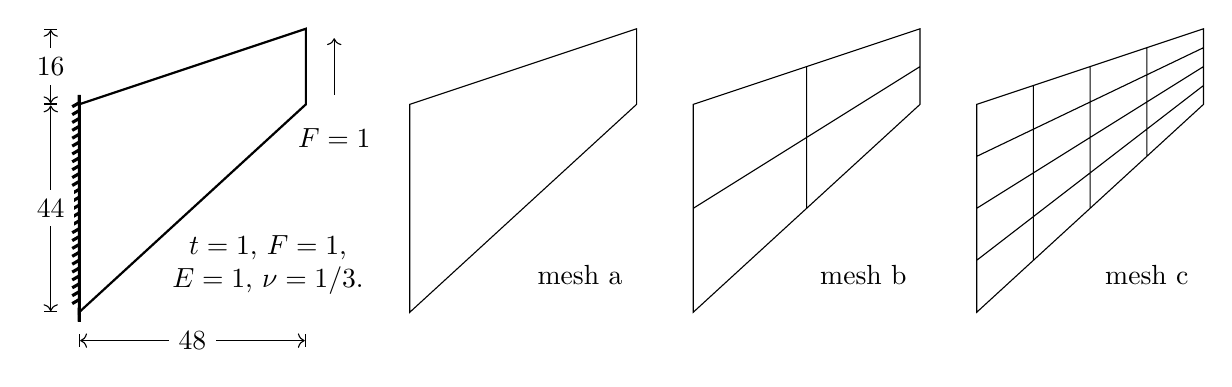
\begin{tikzpicture}[scale=.6]
\FixedSupport[-90]{0,2.2}{6}
\draw[thick](0,0)--(4.8,4.4)--(4.8,6)--(0,4.4)--cycle;
\draw[|<->|](-.6,0)--(-.6,4.4)node[midway,fill=white]{$44$};
\draw[|<->|](0,-.6)--(4.8,-.6)node[midway,fill=white]{$48$};
\draw[|<->|](-.6,4.4)--(-.6,6)node[midway,fill=white]{$16$};
\draw[->](5.4,4.6)node[below=3mm]{$F=1$}--++(0,1.2);
\node[align=center]at(4,1){$t=1$, $F=1$,\\$E=1$, $\nu=1/3$.};
\begin{scope}[xshift=70mm]
\draw(0,0)--(4.8,4.4)--(4.8,6)--(0,4.4)--cycle;
\node[align=center]at(3.6,.8){mesh a};
\end{scope}
\begin{scope}[xshift=130mm]
\draw(0,0)--(4.8,4.4)--(4.8,6)--(0,4.4)--cycle
(0,2.2)--(4.8,5.2)(2.4,2.2)--(2.4,5.2);
\node[align=center]at(3.6,.8){mesh b};
\end{scope}
\begin{scope}[xshift=190mm]
\draw(0,0)--(4.8,4.4)--(4.8,6)--(0,4.4)--cycle
(0,2.2)--(4.8,5.2)(2.4,2.2)--(2.4,5.2)
(1.2,1.1)--(1.2,4.8)
(3.6,3.3)--(3.6,5.6)
(0,1.1)--(4.8,4.8)
(0,3.3)--(4.8,5.6);
\node[align=center]at(3.6,.8){mesh c};
\end{scope}
\end{tikzpicture}
\caption{Cook's skew beam}\label{fig:cooks}
\end{figure}
Numerical results are shown in \tabref{table:cooks}. Similar to the previous curved beam, GCMQ shows a good coarse mesh accuracy. For a \numproduct{4x4} mesh grid, GCMQ can produce the best result compared to all existing four-node membranes. Since the distribution of the end force is not given, a uniformly distributed pattern is assumed. Better results can be obtained by averaging tip deflections for dense mesh grids.
\begin{table}[htb]
\centering\scriptsize
\caption{averaged tip deflection and error of Cook's skew beam}\label{table:cooks}
\begin{tabular}{lrrrrrr}
	\toprule
	                       & \multicolumn{2}{c}{mesh a} & \multicolumn{2}{c}{mesh b} & \multicolumn{2}{c}{mesh c} \\
	                       &   $v$ &      \si{\percent} &   $v$ &      \si{\percent} &   $v$ &      \si{\percent} \\ \midrule
	Q4                     &  5.97 &               75.1 & 11.85 &               50.5 & 18.30 &               23.6 \\
	Q8                     & 17.14 &               28.5 & 22.72 &                5.2 & 23.71 &                1.0 \\
	PS                     & 16.73 &               30.2 & 21.13 &               11.8 & 23.02 &                3.9 \\
	GQ12                   & 16.25 &               32.2 & 20.89 &               12.8 & 23.06 &                3.8 \\
	GQ12M                  & 20.31 &               15.2 & 21.69 &                9.5 & 23.30 &                2.8 \\
	QE2                    & 19.13 &               20.2 & 21.35 &               10.9 & 23.04 &                3.8 \\
	D-Type                 & 14.07 &               41.3 & 20.68 &               13.7 & 22.98 &                4.1 \\
	HSFQ4                  & 21.01 &               12.1 & 22.55 &                5.9 & 23.44 &                2.2 \\
	\citet{Pimpinelli2004} & 15.95 &               33.4 & 21.02 &               12.3 & 23.01 &                4.0 \\
	\citet{Choi2006}       &     - &                  - & 22.55 &                5.9 & 23.44 &                2.2 \\
	\citet{Madeo2012}      &     - &                  - & 22.14 &                7.6 & 23.42 &                2.3 \\
	\citet{Boutagouga2016} &     - &                  - & 22.09 &                7.8 & 23.30 &                2.8 \\
	\citet{Zouari2016}     &     - &                  - & 21.37 &               10.8 & 23.06 &                3.8 \\
	US-ATFQ4               &     - &                  - & 22.76 &                5.0 & 23.43 &                2.2 \\
	GCMQ-I                 & 19.94 &               16.8 & 22.03 &                8.0 & 23.41 &                2.3 \\
	GCMQ-L                 & 19.21 &               19.8 & 22.03 &                8.0 & 23.43 &                2.2 \\
	GCMQ-G                 & 19.19 &               19.9 & 22.41 &                6.5 & 23.52 &                1.8 \\  \midrule
	ref.                   & 23.96 &                    &       &                    &       &                    \\ \bottomrule
\end{tabular}
\end{table}
\subsubsection{Curved Beam}
Convergence can be illustrated by mesh refinement with examples that can be solved analytically. \figref{fig:curved_beam} shows a curved beam subjected to end force.
\begin{figure}[htb]
\centering\footnotesize
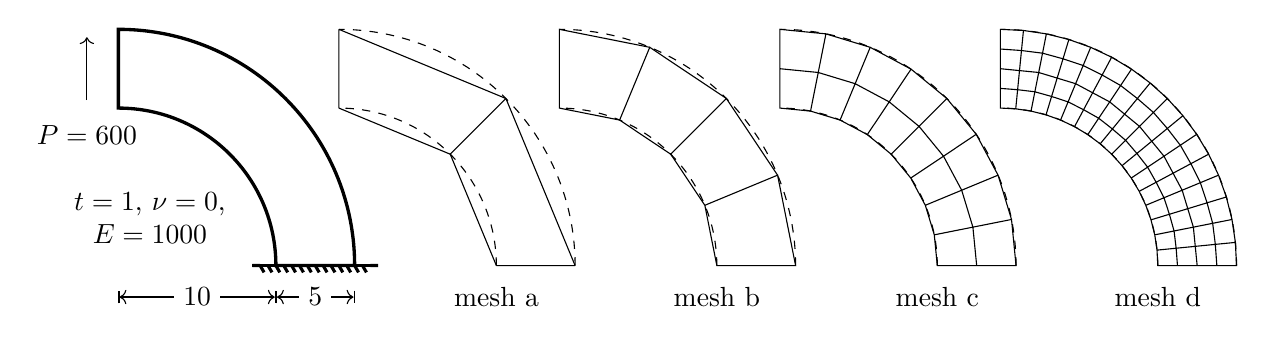
\begin{tikzpicture}[scale=2]
\FixedSupport{1.25,0}
\draw[very thick](1,0)arc(0:90:1)--++(0,.5)arc(90:0:1.5)--cycle;
\draw[|<->|](0,-.2)--++(1,0)node[midway,fill=white]{$10$};
\draw[|<->|](1,-.2)--++(.5,0)node[midway,fill=white]{$5$};
\draw[->](-.2,1.05)node[below=2mm]{$P=600$}--++(0,.4);
\node[align=center]at(.2,.3){$t=1$, $\nu=0$,\\$E=1000$};
\begin{scope}[xshift=14mm]
\coordinate(N1)at(1.0000,0.0000);
\coordinate(N2)at(1.5000,0.0000);
\coordinate(N3)at(0.0000,1.5000);
\coordinate(N4)at(0.0000,1.0000);
\coordinate(N18)at(0.7071,0.7071);
\coordinate(N33)at(1.0607,1.0607);
\draw[dashed](1,0)arc(0:90:1);
\draw[dashed](1.5,0)arc(0:90:1.5);
\draw(N1)--(N2)(N4)--(N3)
(N1)--(N18)--(N4)
(N2)--(N33)--(N3)
(N18)--(N33);
\node at(1,-.2){mesh a};
\end{scope}
\begin{scope}[xshift=28mm]
\coordinate(N1)at(1.0000,0.0000);
\coordinate(N2)at(1.5000,0.0000);
\coordinate(N3)at(0.9239,0.3827);
\coordinate(N4)at(1.3858,0.5740);
\coordinate(N5)at(0.7071,0.7071);
\coordinate(N6)at(1.0607,1.0607);
\coordinate(N7)at(0.3827,0.9239);
\coordinate(N8)at(0.5740,1.3858);
\coordinate(N9)at(0.0000,1.0000);
\coordinate(N10)at(0.0000,1.5000);
\draw[dashed](1,0)arc(0:90:1);
\draw[dashed](1.5,0)arc(0:90:1.5);
\draw
(N1)--(N2)--(N4)--(N3)--cycle
(N3)--(N4)--(N6)--(N5)--cycle
(N5)--(N6)--(N8)--(N7)--cycle
(N7)--(N8)--(N10)--(N9)--cycle;
\node at(1,-.2){mesh b};
\end{scope}
\begin{scope}[xshift=42mm]
\coordinate(N1)at(1.0000,0.0000);
\coordinate(N2)at(1.5000,0.0000);
\coordinate(N3)at(0.0000,1.5000);
\coordinate(N4)at(0.0000,1.0000);
\coordinate(N5)at(0.0000,1.2500);
\coordinate(N6)at(1.2500,0.0000);
\coordinate(N7)at(0.9808,0.1951);
\coordinate(N8)at(0.9239,0.3827);
\coordinate(N9)at(0.8315,0.5556);
\coordinate(N10)at(0.7071,0.7071);
\coordinate(N11)at(0.5556,0.8315);
\coordinate(N12)at(0.3827,0.9239);
\coordinate(N13)at(0.1951,0.9808);
\coordinate(N14)at(1.4712,0.2926);
\coordinate(N15)at(1.3858,0.5740);
\coordinate(N16)at(1.2472,0.8334);
\coordinate(N17)at(1.0607,1.0607);
\coordinate(N18)at(0.8334,1.2472);
\coordinate(N19)at(0.5740,1.3858);
\coordinate(N20)at(0.2926,1.4712);
\coordinate(N21)at(1.2260,0.2439);
\coordinate(N22)at(1.1548,0.4784);
\coordinate(N23)at(1.0393,0.6945);
\coordinate(N24)at(0.8839,0.8839);
\coordinate(N25)at(0.6945,1.0393);
\coordinate(N26)at(0.4784,1.1548);
\coordinate(N27)at(0.2439,1.2260);
\draw[dashed](1,0)arc(0:90:1);
\draw[dashed](1.5,0)arc(0:90:1.5);
\draw
(N2)--(N14)--(N21)--(N6)--cycle
(N6)--(N21)--(N7)--(N1)--cycle
(N14)--(N15)--(N22)--(N21)--cycle
(N21)--(N22)--(N8)--(N7)--cycle
(N15)--(N16)--(N23)--(N22)--cycle
(N22)--(N23)--(N9)--(N8)--cycle
(N16)--(N17)--(N24)--(N23)--cycle
(N23)--(N24)--(N10)--(N9)--cycle
(N17)--(N18)--(N25)--(N24)--cycle
(N24)--(N25)--(N11)--(N10)--cycle
(N18)--(N19)--(N26)--(N25)--cycle
(N25)--(N26)--(N12)--(N11)--cycle
(N19)--(N20)--(N27)--(N26)--cycle
(N26)--(N27)--(N13)--(N12)--cycle
(N20)--(N3)--(N5)--(N27)--cycle
(N27)--(N5)--(N4)--(N13)--cycle;
\node at(1,-.2){mesh c};
\end{scope}
\begin{scope}[xshift=56mm]
\coordinate(N1)at(1.0000,0.0000);
\coordinate(N2)at(1.5000,0.0000);
\coordinate(N3)at(0.0000,1.5000);
\coordinate(N4)at(0.0000,1.0000);
\coordinate(N5)at(0.0000,1.1250);
\coordinate(N6)at(0.0000,1.2500);
\coordinate(N7)at(0.0000,1.3750);
\coordinate(N8)at(1.1250,0.0000);
\coordinate(N9)at(1.2500,0.0000);
\coordinate(N10)at(1.3750,0.0000);
\coordinate(N11)at(0.9952,0.0980);
\coordinate(N12)at(0.9808,0.1951);
\coordinate(N13)at(0.9569,0.2903);
\coordinate(N14)at(0.9239,0.3827);
\coordinate(N15)at(0.8819,0.4714);
\coordinate(N16)at(0.8315,0.5556);
\coordinate(N17)at(0.7730,0.6344);
\coordinate(N18)at(0.7071,0.7071);
\coordinate(N19)at(0.6344,0.7730);
\coordinate(N20)at(0.5556,0.8315);
\coordinate(N21)at(0.4714,0.8819);
\coordinate(N22)at(0.3827,0.9239);
\coordinate(N23)at(0.2903,0.9569);
\coordinate(N24)at(0.1951,0.9808);
\coordinate(N25)at(0.0980,0.9952);
\coordinate(N26)at(1.4928,0.1470);
\coordinate(N27)at(1.4712,0.2926);
\coordinate(N28)at(1.4354,0.4354);
\coordinate(N29)at(1.3858,0.5740);
\coordinate(N30)at(1.3229,0.7071);
\coordinate(N31)at(1.2472,0.8334);
\coordinate(N32)at(1.1595,0.9516);
\coordinate(N33)at(1.0607,1.0607);
\coordinate(N34)at(0.9516,1.1595);
\coordinate(N35)at(0.8334,1.2472);
\coordinate(N36)at(0.7071,1.3229);
\coordinate(N37)at(0.5740,1.3858);
\coordinate(N38)at(0.4354,1.4354);
\coordinate(N39)at(0.2926,1.4712);
\coordinate(N40)at(0.1470,1.4928);
\coordinate(N41)at(1.2260,0.2439);
\coordinate(N42)at(1.1548,0.4784);
\coordinate(N43)at(1.0393,0.6945);
\coordinate(N44)at(0.8839,0.8839);
\coordinate(N45)at(0.6945,1.0393);
\coordinate(N46)at(0.4784,1.1548);
\coordinate(N47)at(0.2439,1.2260);
\coordinate(N48)at(1.3486,0.2682);
\coordinate(N49)at(1.2380,0.1219);
\coordinate(N50)at(1.3654,0.1345);
\coordinate(N51)at(1.1034,0.2195);
\coordinate(N52)at(1.1166,0.1100);
\coordinate(N53)at(1.2703,0.5262);
\coordinate(N54)at(1.1904,0.3611);
\coordinate(N55)at(1.3129,0.3983);
\coordinate(N56)at(1.0394,0.4305);
\coordinate(N57)at(1.0737,0.3257);
\coordinate(N58)at(1.1433,0.7639);
\coordinate(N59)at(1.0971,0.5864);
\coordinate(N60)at(1.2100,0.6468);
\coordinate(N61)at(0.9354,0.6250);
\coordinate(N62)at(0.9895,0.5289);
\coordinate(N63)at(0.9723,0.9723);
\coordinate(N64)at(0.9616,0.7892);
\coordinate(N65)at(1.0606,0.8704);
\coordinate(N66)at(0.7955,0.7955);
\coordinate(N67)at(0.8673,0.7118);
\coordinate(N68)at(0.7639,1.1433);
\coordinate(N69)at(0.7892,0.9616);
\coordinate(N70)at(0.8704,1.0606);
\coordinate(N71)at(0.6250,0.9354);
\coordinate(N72)at(0.7118,0.8673);
\coordinate(N73)at(0.5262,1.2703);
\coordinate(N74)at(0.5864,1.0971);
\coordinate(N75)at(0.6468,1.2100);
\coordinate(N76)at(0.4305,1.0394);
\coordinate(N77)at(0.5289,0.9895);
\coordinate(N78)at(0.2682,1.3486);
\coordinate(N79)at(0.3611,1.1904);
\coordinate(N80)at(0.3983,1.3129);
\coordinate(N81)at(0.2195,1.1034);
\coordinate(N82)at(0.3257,1.0737);
\coordinate(N83)at(0.1219,1.2380);
\coordinate(N84)at(0.1345,1.3654);
\coordinate(N85)at(0.1100,1.1166);
\draw[dashed](1,0)arc(0:90:1);
\draw[dashed](1.5,0)arc(0:90:1.5);
\draw
(N2)--(N26)--(N50)--(N10)--cycle
(N26)--(N27)--(N48)--(N50)--cycle
(N50)--(N48)--(N41)--(N49)--cycle
(N10)--(N50)--(N49)--(N9)--cycle
(N9)--(N49)--(N52)--(N8)--cycle
(N49)--(N41)--(N51)--(N52)--cycle
(N52)--(N51)--(N12)--(N11)--cycle
(N8)--(N52)--(N11)--(N1)--cycle
(N27)--(N28)--(N55)--(N48)--cycle
(N28)--(N29)--(N53)--(N55)--cycle
(N55)--(N53)--(N42)--(N54)--cycle
(N48)--(N55)--(N54)--(N41)--cycle
(N41)--(N54)--(N57)--(N51)--cycle
(N54)--(N42)--(N56)--(N57)--cycle
(N57)--(N56)--(N14)--(N13)--cycle
(N51)--(N57)--(N13)--(N12)--cycle
(N29)--(N30)--(N60)--(N53)--cycle
(N30)--(N31)--(N58)--(N60)--cycle
(N60)--(N58)--(N43)--(N59)--cycle
(N53)--(N60)--(N59)--(N42)--cycle
(N42)--(N59)--(N62)--(N56)--cycle
(N59)--(N43)--(N61)--(N62)--cycle
(N62)--(N61)--(N16)--(N15)--cycle
(N56)--(N62)--(N15)--(N14)--cycle
(N31)--(N32)--(N65)--(N58)--cycle
(N32)--(N33)--(N63)--(N65)--cycle
(N65)--(N63)--(N44)--(N64)--cycle
(N58)--(N65)--(N64)--(N43)--cycle
(N43)--(N64)--(N67)--(N61)--cycle
(N64)--(N44)--(N66)--(N67)--cycle
(N67)--(N66)--(N18)--(N17)--cycle
(N61)--(N67)--(N17)--(N16)--cycle
(N33)--(N34)--(N70)--(N63)--cycle
(N34)--(N35)--(N68)--(N70)--cycle
(N70)--(N68)--(N45)--(N69)--cycle
(N63)--(N70)--(N69)--(N44)--cycle
(N44)--(N69)--(N72)--(N66)--cycle
(N69)--(N45)--(N71)--(N72)--cycle
(N72)--(N71)--(N20)--(N19)--cycle
(N66)--(N72)--(N19)--(N18)--cycle
(N35)--(N36)--(N75)--(N68)--cycle
(N36)--(N37)--(N73)--(N75)--cycle
(N75)--(N73)--(N46)--(N74)--cycle
(N68)--(N75)--(N74)--(N45)--cycle
(N45)--(N74)--(N77)--(N71)--cycle
(N74)--(N46)--(N76)--(N77)--cycle
(N77)--(N76)--(N22)--(N21)--cycle
(N71)--(N77)--(N21)--(N20)--cycle
(N37)--(N38)--(N80)--(N73)--cycle
(N38)--(N39)--(N78)--(N80)--cycle
(N80)--(N78)--(N47)--(N79)--cycle
(N73)--(N80)--(N79)--(N46)--cycle
(N46)--(N79)--(N82)--(N76)--cycle
(N79)--(N47)--(N81)--(N82)--cycle
(N82)--(N81)--(N24)--(N23)--cycle
(N76)--(N82)--(N23)--(N22)--cycle
(N39)--(N40)--(N84)--(N78)--cycle
(N40)--(N3)--(N7)--(N84)--cycle
(N84)--(N7)--(N6)--(N83)--cycle
(N78)--(N84)--(N83)--(N47)--cycle
(N47)--(N83)--(N85)--(N81)--cycle
(N83)--(N6)--(N5)--(N85)--cycle
(N85)--(N5)--(N4)--(N25)--cycle
(N81)--(N85)--(N25)--(N24)--cycle;
\node at(1,-.2){mesh d};
\end{scope}
\end{tikzpicture}
\caption{curved beam subjected to tip load}\label{fig:curved_beam}
\end{figure}
The deflection of the free end is given analytically by
\begin{gather}
v=\dfrac{P\pi}{E}\cdot\dfrac{a^2+b^2}{\left(a^2-b^2\right)+(a^2+b^2)\log\dfrac{b}{a}}.
\end{gather}
The derivation can be seen elsewhere \citep{Timoshenko1970}. For the geometry and material properties shown in \figref{fig:curved_beam}, where $a=10$ and $b=15$,
\begin{gather}
v=\dfrac{600}{1000}\cdot\dfrac{10^2+15^2}{\left(10^2-15^2\right)+(10^2+15^2)\log1.5}\cdot\pi\approx90.41.
\end{gather}
It shall be noted that the above analytical solution is obtained by applying traction boundary condition $\displaystyle\int\tau~\md{A}=P$ on the free end, the actual distribution of $\tau$ is unknown. In the following numerical examples, a uniformly distributed shear force is assumed.

\begin{table}[H]
\centering\scriptsize
\caption{averaged tip deflection and error of a curved beam}\label{table:curved_beam}
\begin{tabular}{lrrrrrrrr}
	\toprule
	         & \multicolumn{2}{c}{mesh a} & \multicolumn{2}{c}{mesh b} & \multicolumn{2}{c}{mesh c} & \multicolumn{2}{c}{mesh d} \\
	element  &   $v$ &      \si{\percent} &   $v$ &      \si{\percent} &   $v$ &      \si{\percent} &   $v$ &      \si{\percent} \\ \midrule
	Q4       & 22.36 &              75.27 & 57.90 &              35.96 & 79.29 &              12.30 & 87.26 &               3.49 \\
	PS       & 51.16 &              43.42 & 84.52 &               6.52 & 88.41 &               2.20 & 89.79 &               0.68 \\
	QE2      & 51.32 &              43.23 & 84.53 &               6.50 & 88.41 &               2.20 & 89.79 &               0.68 \\
	GQ12     & 83.70 &               7.42 & 89.07 &               1.48 & 89.81 &               0.66 & 90.20 &               0.23 \\
	US-ATFQ4 &     - &                  - & 86.30 &               4.54 &     - &                  - &     - &                  - \\
	AGQ-I    &     - &                  - & 91.88 &              -1.63 &     - &                  - &     - &                  - \\
	AGQ-II   &     - &                  - & 86.93 &               3.85 &     - &                  - &     - &                  - \\
	GCMQ-I   & 85.31 &               5.64 & 87.17 &               3.58 & 89.88 &               0.58 & 90.26 &               0.16 \\
	GCMQ-L   & 85.52 &               5.40 & 88.74 &               1.84 & 89.94 &               0.51 & 90.26 &               0.16 \\
	GCMQ-G   & 86.72 &               4.08 & 89.83 &               0.64 & 90.05 &               0.39 & 90.27 &               0.15 \\ \midrule
	ref.     & 90.41 &                    &       &                    &       &                    &       &                    \\ \bottomrule
\end{tabular}
\end{table}
Numerical results and comparisons with other elements are presented in \tabref{table:curved_beam}. For the not-even-close-to-geometry mesh grid with only two elements defined, the error is around \SI{5}{\percent} which is acceptable. This indicates GCMQ has a decent performance under coarse mesh configurations.
\subsubsection{Plate With Circular Hole}\label{plate_with_hole_example}
As illustrated in \figref{fig:plate_with_hole}, for a sufficiently large plate with a circular hole subjected to uniform tension, the stress distribution around the hole can be obtained by the Kirsch's solution \citep[see][pg. 80]{Timoshenko1970}. The normal stress $\sigma_y$ along $x$-axis is
\begin{gather}\label{kirsch_a}
\sigma_y=q\left(\dfrac{1}{2}\dfrac{a^2}{\rho^2}-\dfrac{3}{2}\dfrac{a^4}{\rho^4}\right),
\end{gather}
while the normal stress $\sigma_x$ along $y$-axis is
\begin{gather}\label{kirsch_b}
\sigma_x=q\left(1+\dfrac{1}{2}\dfrac{a^2}{\rho^2}+\dfrac{3}{2}\dfrac{a^4}{\rho^4}\right),
\end{gather}
where $\rho$ is the polar coordinate.
\begin{figure}[htb]
\centering\footnotesize
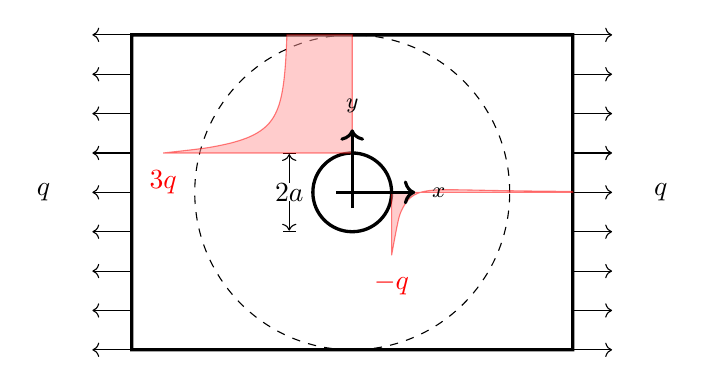
\begin{tikzpicture}
\def\a{2.0};\def\b{1.4*\a}
\draw[very thick](-\b,-\a)rectangle(\b,\a)(0,0)circle(\a/4);
\draw[dashed](0,0)circle(\a);
\foreach\x in{-2,-1.5,-1,-.5,0,.5,1,1.5,2}{
\draw[->](-\b,\x)--++(-.5,0);
\draw[->](\b,\x)--++(.5,0);
}
\node at(-1.4*\b,0){$q$};
\node at(1.4*\b,0){$q$};
\draw[|<->|](-\a/2.5,-\a/4)--++(0,\a/2)node[midway,fill=white,inner sep=0]{$2a$};
\draw[domain=\a/4:\b,smooth,variable=\x,red,fill=red!40,opacity=.5]plot({\x},{.8*(\a*\a/\x/\x/32-3/512*\a*\a*\a*\a/\x/\x/\x/\x)})--(\b,0)--(\a/4,0)--cycle node[opacity=1,below=1mm]{$-q$};
\draw[domain=\a/4:\a,smooth,variable=\x,red,fill=red!40,opacity=.5]plot({.8*(-1-\a*\a/\x/\x/32-3/512*\a*\a*\a*\a/\x/\x/\x/\x)},{\x})--(0,\a)--(0,\a/4)--cycle node[opacity=1,below=1mm]{$3q$};
\CoorOrigin{0,0}
\end{tikzpicture}
\caption{plate with circular hole}\label{fig:plate_with_hole}
\end{figure}

A quarter of the plate is analysed using the mesh grids shown in \figref{fig:plate_with_hole_mesh} and a plane stress isotropic elastic material model with Young's modulus of $E=1000$ and Poisson's ratio of $\nu=0.2$.
\begin{figure}[htb]
\centering\scriptsize
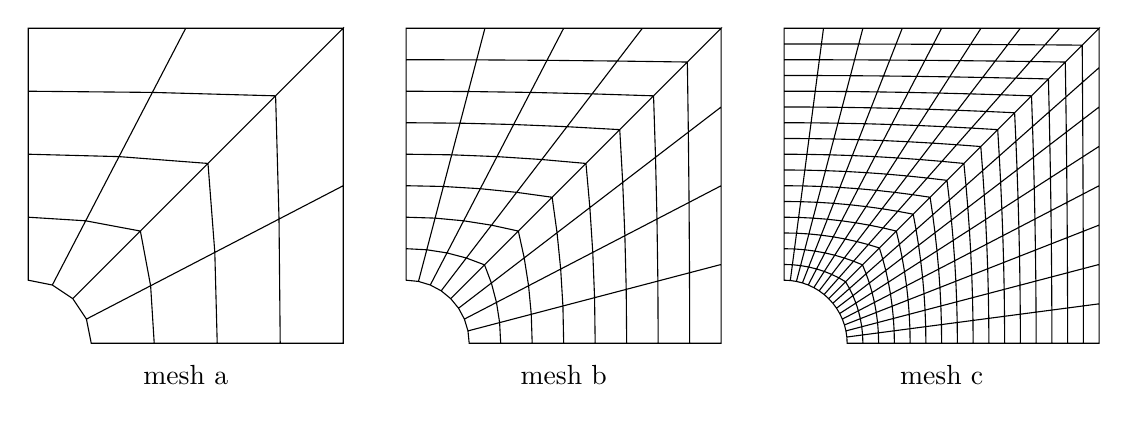
\begin{tikzpicture}[scale=.8]
\node at(2.5,-.5){mesh a};
\coordinate(N1)at(5.0000,5.0000);
\coordinate(N2)at(0.7071,0.7071);
\coordinate(N3)at(1.0000,0.0000);
\coordinate(N4)at(5.0000,0.0000);
\coordinate(N5)at(0.0000,5.0000);
\coordinate(N6)at(0.0000,1.0000);
\coordinate(N7)at(3.9268,3.9268);
\coordinate(N8)at(2.8536,2.8536);
\coordinate(N9)at(1.7803,1.7803);
\coordinate(N10)at(0.9239,0.3827);
\coordinate(N11)at(2.0000,0.0000);
\coordinate(N12)at(3.0000,0.0000);
\coordinate(N13)at(4.0000,0.0000);
\coordinate(N14)at(5.0000,2.5000);
\coordinate(N15)at(2.5000,5.0000);
\coordinate(N16)at(0.0000,4.0000);
\coordinate(N17)at(0.0000,3.0000);
\coordinate(N18)at(0.0000,2.0000);
\coordinate(N19)at(0.3827,0.9239);
\coordinate(N20)at(3.9810,1.9707);
\coordinate(N21)at(2.9619,1.4413);
\coordinate(N22)at(1.9429,0.9120);
\coordinate(N23)at(0.9120,1.9429);
\coordinate(N24)at(1.4413,2.9619);
\coordinate(N25)at(1.9707,3.9810);
\draw
(N1)--(N7)--(N20)--(N14)--cycle
(N7)--(N8)--(N21)--(N20)--cycle
(N8)--(N9)--(N22)--(N21)--cycle
(N9)--(N2)--(N10)--(N22)--cycle
(N14)--(N20)--(N13)--(N4)--cycle
(N20)--(N21)--(N12)--(N13)--cycle
(N21)--(N22)--(N11)--(N12)--cycle
(N22)--(N10)--(N3)--(N11)--cycle
(N2)--(N9)--(N23)--(N19)--cycle
(N9)--(N8)--(N24)--(N23)--cycle
(N8)--(N7)--(N25)--(N24)--cycle
(N7)--(N1)--(N15)--(N25)--cycle
(N19)--(N23)--(N18)--(N6)--cycle
(N23)--(N24)--(N17)--(N18)--cycle
(N24)--(N25)--(N16)--(N17)--cycle
(N25)--(N15)--(N5)--(N16)--cycle;
\begin{scope}[xshift=60mm]
\node at(2.5,-.5){mesh b};
\coordinate(N1)at(5.0000,5.0000);
\coordinate(N2)at(0.7071,0.7071);
\coordinate(N3)at(1.0000,0.0000);
\coordinate(N4)at(5.0000,0.0000);
\coordinate(N5)at(0.0000,5.0000);
\coordinate(N6)at(0.0000,1.0000);
\coordinate(N7)at(4.4634,4.4634);
\coordinate(N8)at(3.9268,3.9268);
\coordinate(N9)at(3.3902,3.3902);
\coordinate(N10)at(2.8536,2.8536);
\coordinate(N11)at(2.3169,2.3169);
\coordinate(N12)at(1.7803,1.7803);
\coordinate(N13)at(1.2437,1.2437);
\coordinate(N14)at(0.8315,0.5556);
\coordinate(N15)at(0.9239,0.3827);
\coordinate(N16)at(0.9808,0.1951);
\coordinate(N17)at(1.5000,0.0000);
\coordinate(N18)at(2.0000,0.0000);
\coordinate(N19)at(2.5000,0.0000);
\coordinate(N20)at(3.0000,0.0000);
\coordinate(N21)at(3.5000,0.0000);
\coordinate(N22)at(4.0000,0.0000);
\coordinate(N23)at(4.5000,0.0000);
\coordinate(N24)at(5.0000,1.2500);
\coordinate(N25)at(5.0000,2.5000);
\coordinate(N26)at(5.0000,3.7500);
\coordinate(N27)at(3.7500,5.0000);
\coordinate(N28)at(2.5000,5.0000);
\coordinate(N29)at(1.2500,5.0000);
\coordinate(N30)at(0.0000,4.5000);
\coordinate(N31)at(0.0000,4.0000);
\coordinate(N32)at(0.0000,3.5000);
\coordinate(N33)at(0.0000,3.0000);
\coordinate(N34)at(0.0000,2.5000);
\coordinate(N35)at(0.0000,2.0000);
\coordinate(N36)at(0.0000,1.5000);
\coordinate(N37)at(0.1951,0.9808);
\coordinate(N38)at(0.3827,0.9239);
\coordinate(N39)at(0.5556,0.8315);
\coordinate(N40)at(4.4789,3.3507);
\coordinate(N41)at(3.9579,2.9514);
\coordinate(N42)at(3.4368,2.5521);
\coordinate(N43)at(2.9157,2.1528);
\coordinate(N44)at(2.3947,1.7535);
\coordinate(N45)at(1.8736,1.3542);
\coordinate(N46)at(1.3525,0.9549);
\coordinate(N47)at(4.4905,2.2353);
\coordinate(N48)at(3.9810,1.9707);
\coordinate(N49)at(3.4715,1.7060);
\coordinate(N50)at(2.9619,1.4413);
\coordinate(N51)at(2.4524,1.1767);
\coordinate(N52)at(1.9429,0.9120);
\coordinate(N53)at(1.4334,0.6473);
\coordinate(N54)at(4.4976,1.1181);
\coordinate(N55)at(3.9952,0.9863);
\coordinate(N56)at(3.4928,0.8544);
\coordinate(N57)at(2.9904,0.7225);
\coordinate(N58)at(2.4880,0.5907);
\coordinate(N59)at(1.9856,0.4588);
\coordinate(N60)at(1.4832,0.3270);
\coordinate(N61)at(0.9549,1.3525);
\coordinate(N62)at(1.3542,1.8736);
\coordinate(N63)at(1.7535,2.3947);
\coordinate(N64)at(2.1528,2.9157);
\coordinate(N65)at(2.5521,3.4368);
\coordinate(N66)at(2.9514,3.9579);
\coordinate(N67)at(3.3507,4.4789);
\coordinate(N68)at(0.6473,1.4334);
\coordinate(N69)at(0.9120,1.9429);
\coordinate(N70)at(1.1767,2.4524);
\coordinate(N71)at(1.4413,2.9619);
\coordinate(N72)at(1.7060,3.4715);
\coordinate(N73)at(1.9707,3.9810);
\coordinate(N74)at(2.2353,4.4905);
\coordinate(N75)at(0.3270,1.4832);
\coordinate(N76)at(0.4588,1.9856);
\coordinate(N77)at(0.5907,2.4880);
\coordinate(N78)at(0.7225,2.9904);
\coordinate(N79)at(0.8544,3.4928);
\coordinate(N80)at(0.9863,3.9952);
\coordinate(N81)at(1.1181,4.4976);
\draw
(N1)--(N7)--(N40)--(N26)--cycle
(N7)--(N8)--(N41)--(N40)--cycle
(N8)--(N9)--(N42)--(N41)--cycle
(N9)--(N10)--(N43)--(N42)--cycle
(N10)--(N11)--(N44)--(N43)--cycle
(N11)--(N12)--(N45)--(N44)--cycle
(N12)--(N13)--(N46)--(N45)--cycle
(N13)--(N2)--(N14)--(N46)--cycle
(N26)--(N40)--(N47)--(N25)--cycle
(N40)--(N41)--(N48)--(N47)--cycle
(N41)--(N42)--(N49)--(N48)--cycle
(N42)--(N43)--(N50)--(N49)--cycle
(N43)--(N44)--(N51)--(N50)--cycle
(N44)--(N45)--(N52)--(N51)--cycle
(N45)--(N46)--(N53)--(N52)--cycle
(N46)--(N14)--(N15)--(N53)--cycle
(N25)--(N47)--(N54)--(N24)--cycle
(N47)--(N48)--(N55)--(N54)--cycle
(N48)--(N49)--(N56)--(N55)--cycle
(N49)--(N50)--(N57)--(N56)--cycle
(N50)--(N51)--(N58)--(N57)--cycle
(N51)--(N52)--(N59)--(N58)--cycle
(N52)--(N53)--(N60)--(N59)--cycle
(N53)--(N15)--(N16)--(N60)--cycle
(N24)--(N54)--(N23)--(N4)--cycle
(N54)--(N55)--(N22)--(N23)--cycle
(N55)--(N56)--(N21)--(N22)--cycle
(N56)--(N57)--(N20)--(N21)--cycle
(N57)--(N58)--(N19)--(N20)--cycle
(N58)--(N59)--(N18)--(N19)--cycle
(N59)--(N60)--(N17)--(N18)--cycle
(N60)--(N16)--(N3)--(N17)--cycle
(N2)--(N13)--(N61)--(N39)--cycle
(N13)--(N12)--(N62)--(N61)--cycle
(N12)--(N11)--(N63)--(N62)--cycle
(N11)--(N10)--(N64)--(N63)--cycle
(N10)--(N9)--(N65)--(N64)--cycle
(N9)--(N8)--(N66)--(N65)--cycle
(N8)--(N7)--(N67)--(N66)--cycle
(N7)--(N1)--(N27)--(N67)--cycle
(N39)--(N61)--(N68)--(N38)--cycle
(N61)--(N62)--(N69)--(N68)--cycle
(N62)--(N63)--(N70)--(N69)--cycle
(N63)--(N64)--(N71)--(N70)--cycle
(N64)--(N65)--(N72)--(N71)--cycle
(N65)--(N66)--(N73)--(N72)--cycle
(N66)--(N67)--(N74)--(N73)--cycle
(N67)--(N27)--(N28)--(N74)--cycle
(N38)--(N68)--(N75)--(N37)--cycle
(N68)--(N69)--(N76)--(N75)--cycle
(N69)--(N70)--(N77)--(N76)--cycle
(N70)--(N71)--(N78)--(N77)--cycle
(N71)--(N72)--(N79)--(N78)--cycle
(N72)--(N73)--(N80)--(N79)--cycle
(N73)--(N74)--(N81)--(N80)--cycle
(N74)--(N28)--(N29)--(N81)--cycle
(N37)--(N75)--(N36)--(N6)--cycle
(N75)--(N76)--(N35)--(N36)--cycle
(N76)--(N77)--(N34)--(N35)--cycle
(N77)--(N78)--(N33)--(N34)--cycle
(N78)--(N79)--(N32)--(N33)--cycle
(N79)--(N80)--(N31)--(N32)--cycle
(N80)--(N81)--(N30)--(N31)--cycle
(N81)--(N29)--(N5)--(N30)--cycle;
\end{scope}
\begin{scope}[xshift=120mm]
\node at(2.5,-.5){mesh c};
\coordinate(N1)at(5.0000,5.0000);
\coordinate(N2)at(0.7071,0.7071);
\coordinate(N3)at(1.0000,0.0000);
\coordinate(N4)at(5.0000,0.0000);
\coordinate(N5)at(0.0000,5.0000);
\coordinate(N6)at(0.0000,1.0000);
\coordinate(N7)at(4.7317,4.7317);
\coordinate(N8)at(4.4634,4.4634);
\coordinate(N9)at(4.1951,4.1951);
\coordinate(N10)at(3.9268,3.9268);
\coordinate(N11)at(3.6585,3.6585);
\coordinate(N12)at(3.3902,3.3902);
\coordinate(N13)at(3.1219,3.1219);
\coordinate(N14)at(2.8536,2.8536);
\coordinate(N15)at(2.5852,2.5852);
\coordinate(N16)at(2.3169,2.3169);
\coordinate(N17)at(2.0486,2.0486);
\coordinate(N18)at(1.7803,1.7803);
\coordinate(N19)at(1.5120,1.5120);
\coordinate(N20)at(1.2437,1.2437);
\coordinate(N21)at(0.9754,0.9754);
\coordinate(N22)at(0.7730,0.6344);
\coordinate(N23)at(0.8315,0.5556);
\coordinate(N24)at(0.8819,0.4714);
\coordinate(N25)at(0.9239,0.3827);
\coordinate(N26)at(0.9569,0.2903);
\coordinate(N27)at(0.9808,0.1951);
\coordinate(N28)at(0.9952,0.0980);
\coordinate(N29)at(1.2500,0.0000);
\coordinate(N30)at(1.5000,0.0000);
\coordinate(N31)at(1.7500,0.0000);
\coordinate(N32)at(2.0000,0.0000);
\coordinate(N33)at(2.2500,0.0000);
\coordinate(N34)at(2.5000,0.0000);
\coordinate(N35)at(2.7500,0.0000);
\coordinate(N36)at(3.0000,0.0000);
\coordinate(N37)at(3.2500,0.0000);
\coordinate(N38)at(3.5000,0.0000);
\coordinate(N39)at(3.7500,0.0000);
\coordinate(N40)at(4.0000,0.0000);
\coordinate(N41)at(4.2500,0.0000);
\coordinate(N42)at(4.5000,0.0000);
\coordinate(N43)at(4.7500,0.0000);
\coordinate(N44)at(5.0000,0.6250);
\coordinate(N45)at(5.0000,1.2500);
\coordinate(N46)at(5.0000,1.8750);
\coordinate(N47)at(5.0000,2.5000);
\coordinate(N48)at(5.0000,3.1250);
\coordinate(N49)at(5.0000,3.7500);
\coordinate(N50)at(5.0000,4.3750);
\coordinate(N51)at(4.3750,5.0000);
\coordinate(N52)at(3.7500,5.0000);
\coordinate(N53)at(3.1250,5.0000);
\coordinate(N54)at(2.5000,5.0000);
\coordinate(N55)at(1.8750,5.0000);
\coordinate(N56)at(1.2500,5.0000);
\coordinate(N57)at(0.6250,5.0000);
\coordinate(N58)at(0.0000,4.7500);
\coordinate(N59)at(0.0000,4.5000);
\coordinate(N60)at(0.0000,4.2500);
\coordinate(N61)at(0.0000,4.0000);
\coordinate(N62)at(0.0000,3.7500);
\coordinate(N63)at(0.0000,3.5000);
\coordinate(N64)at(0.0000,3.2500);
\coordinate(N65)at(0.0000,3.0000);
\coordinate(N66)at(0.0000,2.7500);
\coordinate(N67)at(0.0000,2.5000);
\coordinate(N68)at(0.0000,2.2500);
\coordinate(N69)at(0.0000,2.0000);
\coordinate(N70)at(0.0000,1.7500);
\coordinate(N71)at(0.0000,1.5000);
\coordinate(N72)at(0.0000,1.2500);
\coordinate(N73)at(0.0980,0.9952);
\coordinate(N74)at(0.1951,0.9808);
\coordinate(N75)at(0.2903,0.9569);
\coordinate(N76)at(0.3827,0.9239);
\coordinate(N77)at(0.4714,0.8819);
\coordinate(N78)at(0.5556,0.8315);
\coordinate(N79)at(0.6344,0.7730);
\coordinate(N80)at(4.7358,4.1412);
\coordinate(N81)at(4.4716,3.9074);
\coordinate(N82)at(4.2074,3.6736);
\coordinate(N83)at(3.9433,3.4398);
\coordinate(N84)at(3.6791,3.2061);
\coordinate(N85)at(3.4149,2.9723);
\coordinate(N86)at(3.1507,2.7385);
\coordinate(N87)at(2.8865,2.5047);
\coordinate(N88)at(2.6223,2.2709);
\coordinate(N89)at(2.3581,2.0371);
\coordinate(N90)at(2.0939,1.8033);
\coordinate(N91)at(1.8298,1.5695);
\coordinate(N92)at(1.5656,1.3358);
\coordinate(N93)at(1.3014,1.1020);
\coordinate(N94)at(1.0372,0.8682);
\coordinate(N95)at(4.7395,3.5503);
\coordinate(N96)at(4.4789,3.3507);
\coordinate(N97)at(4.2184,3.1510);
\coordinate(N98)at(3.9579,2.9514);
\coordinate(N99)at(3.6973,2.7517);
\coordinate(N100)at(3.4368,2.5521);
\coordinate(N101)at(3.1763,2.3524);
\coordinate(N102)at(2.9157,2.1528);
\coordinate(N103)at(2.6552,1.9531);
\coordinate(N104)at(2.3947,1.7535);
\coordinate(N105)at(2.1341,1.5538);
\coordinate(N106)at(1.8736,1.3542);
\coordinate(N107)at(1.6131,1.1545);
\coordinate(N108)at(1.3525,0.9549);
\coordinate(N109)at(1.0920,0.7552);
\coordinate(N110)at(4.7426,2.9591);
\coordinate(N111)at(4.4852,2.7933);
\coordinate(N112)at(4.2279,2.6274);
\coordinate(N113)at(3.9705,2.4616);
\coordinate(N114)at(3.7131,2.2957);
\coordinate(N115)at(3.4557,2.1299);
\coordinate(N116)at(3.1983,1.9640);
\coordinate(N117)at(2.9410,1.7982);
\coordinate(N118)at(2.6836,1.6323);
\coordinate(N119)at(2.4262,1.4665);
\coordinate(N120)at(2.1688,1.3006);
\coordinate(N121)at(1.9114,1.1348);
\coordinate(N122)at(1.6541,0.9689);
\coordinate(N123)at(1.3967,0.8031);
\coordinate(N124)at(1.1393,0.6372);
\coordinate(N125)at(4.7452,2.3677);
\coordinate(N126)at(4.4905,2.2353);
\coordinate(N127)at(4.2357,2.1030);
\coordinate(N128)at(3.9810,1.9707);
\coordinate(N129)at(3.7262,1.8383);
\coordinate(N130)at(3.4715,1.7060);
\coordinate(N131)at(3.2167,1.5737);
\coordinate(N132)at(2.9619,1.4413);
\coordinate(N133)at(2.7072,1.3090);
\coordinate(N134)at(2.4524,1.1767);
\coordinate(N135)at(2.1977,1.0443);
\coordinate(N136)at(1.9429,0.9120);
\coordinate(N137)at(1.6882,0.7797);
\coordinate(N138)at(1.4334,0.6473);
\coordinate(N139)at(1.1786,0.5150);
\coordinate(N140)at(4.7473,1.7760);
\coordinate(N141)at(4.4946,1.6769);
\coordinate(N142)at(4.2419,1.5779);
\coordinate(N143)at(3.9892,1.4788);
\coordinate(N144)at(3.7365,1.3798);
\coordinate(N145)at(3.4839,1.2807);
\coordinate(N146)at(3.2312,1.1817);
\coordinate(N147)at(2.9785,1.0826);
\coordinate(N148)at(2.7258,0.9836);
\coordinate(N149)at(2.4731,0.8846);
\coordinate(N150)at(2.2204,0.7855);
\coordinate(N151)at(1.9677,0.6865);
\coordinate(N152)at(1.7150,0.5874);
\coordinate(N153)at(1.4623,0.4884);
\coordinate(N154)at(1.2096,0.3893);
\coordinate(N155)at(4.7488,1.1841);
\coordinate(N156)at(4.4976,1.1181);
\coordinate(N157)at(4.2464,1.0522);
\coordinate(N158)at(3.9952,0.9863);
\coordinate(N159)at(3.7440,0.9203);
\coordinate(N160)at(3.4928,0.8544);
\coordinate(N161)at(3.2416,0.7885);
\coordinate(N162)at(2.9904,0.7225);
\coordinate(N163)at(2.7392,0.6566);
\coordinate(N164)at(2.4880,0.5907);
\coordinate(N165)at(2.2368,0.5247);
\coordinate(N166)at(1.9856,0.4588);
\coordinate(N167)at(1.7344,0.3929);
\coordinate(N168)at(1.4832,0.3270);
\coordinate(N169)at(1.2320,0.2610);
\coordinate(N170)at(4.7497,0.5921);
\coordinate(N171)at(4.4994,0.5591);
\coordinate(N172)at(4.2491,0.5262);
\coordinate(N173)at(3.9988,0.4933);
\coordinate(N174)at(3.7485,0.4603);
\coordinate(N175)at(3.4982,0.4274);
\coordinate(N176)at(3.2479,0.3944);
\coordinate(N177)at(2.9976,0.3615);
\coordinate(N178)at(2.7473,0.3286);
\coordinate(N179)at(2.4970,0.2956);
\coordinate(N180)at(2.2467,0.2627);
\coordinate(N181)at(1.9964,0.2298);
\coordinate(N182)at(1.7461,0.1968);
\coordinate(N183)at(1.4958,0.1639);
\coordinate(N184)at(1.2455,0.1310);
\coordinate(N185)at(0.8682,1.0372);
\coordinate(N186)at(1.1020,1.3014);
\coordinate(N187)at(1.3358,1.5656);
\coordinate(N188)at(1.5695,1.8298);
\coordinate(N189)at(1.8033,2.0939);
\coordinate(N190)at(2.0371,2.3581);
\coordinate(N191)at(2.2709,2.6223);
\coordinate(N192)at(2.5047,2.8865);
\coordinate(N193)at(2.7385,3.1507);
\coordinate(N194)at(2.9723,3.4149);
\coordinate(N195)at(3.2061,3.6791);
\coordinate(N196)at(3.4398,3.9433);
\coordinate(N197)at(3.6736,4.2074);
\coordinate(N198)at(3.9074,4.4716);
\coordinate(N199)at(4.1412,4.7358);
\coordinate(N200)at(0.7552,1.0920);
\coordinate(N201)at(0.9549,1.3525);
\coordinate(N202)at(1.1545,1.6131);
\coordinate(N203)at(1.3542,1.8736);
\coordinate(N204)at(1.5538,2.1341);
\coordinate(N205)at(1.7535,2.3947);
\coordinate(N206)at(1.9531,2.6552);
\coordinate(N207)at(2.1528,2.9157);
\coordinate(N208)at(2.3524,3.1763);
\coordinate(N209)at(2.5521,3.4368);
\coordinate(N210)at(2.7517,3.6973);
\coordinate(N211)at(2.9514,3.9579);
\coordinate(N212)at(3.1510,4.2184);
\coordinate(N213)at(3.3507,4.4789);
\coordinate(N214)at(3.5503,4.7395);
\coordinate(N215)at(0.6372,1.1393);
\coordinate(N216)at(0.8031,1.3967);
\coordinate(N217)at(0.9689,1.6541);
\coordinate(N218)at(1.1348,1.9114);
\coordinate(N219)at(1.3006,2.1688);
\coordinate(N220)at(1.4665,2.4262);
\coordinate(N221)at(1.6323,2.6836);
\coordinate(N222)at(1.7982,2.9410);
\coordinate(N223)at(1.9640,3.1983);
\coordinate(N224)at(2.1299,3.4557);
\coordinate(N225)at(2.2957,3.7131);
\coordinate(N226)at(2.4616,3.9705);
\coordinate(N227)at(2.6274,4.2279);
\coordinate(N228)at(2.7933,4.4852);
\coordinate(N229)at(2.9591,4.7426);
\coordinate(N230)at(0.5150,1.1786);
\coordinate(N231)at(0.6473,1.4334);
\coordinate(N232)at(0.7797,1.6882);
\coordinate(N233)at(0.9120,1.9429);
\coordinate(N234)at(1.0443,2.1977);
\coordinate(N235)at(1.1767,2.4524);
\coordinate(N236)at(1.3090,2.7072);
\coordinate(N237)at(1.4413,2.9619);
\coordinate(N238)at(1.5737,3.2167);
\coordinate(N239)at(1.7060,3.4715);
\coordinate(N240)at(1.8383,3.7262);
\coordinate(N241)at(1.9707,3.9810);
\coordinate(N242)at(2.1030,4.2357);
\coordinate(N243)at(2.2353,4.4905);
\coordinate(N244)at(2.3677,4.7452);
\coordinate(N245)at(0.3893,1.2096);
\coordinate(N246)at(0.4884,1.4623);
\coordinate(N247)at(0.5874,1.7150);
\coordinate(N248)at(0.6865,1.9677);
\coordinate(N249)at(0.7855,2.2204);
\coordinate(N250)at(0.8846,2.4731);
\coordinate(N251)at(0.9836,2.7258);
\coordinate(N252)at(1.0826,2.9785);
\coordinate(N253)at(1.1817,3.2312);
\coordinate(N254)at(1.2807,3.4839);
\coordinate(N255)at(1.3798,3.7365);
\coordinate(N256)at(1.4788,3.9892);
\coordinate(N257)at(1.5779,4.2419);
\coordinate(N258)at(1.6769,4.4946);
\coordinate(N259)at(1.7760,4.7473);
\coordinate(N260)at(0.2610,1.2320);
\coordinate(N261)at(0.3270,1.4832);
\coordinate(N262)at(0.3929,1.7344);
\coordinate(N263)at(0.4588,1.9856);
\coordinate(N264)at(0.5247,2.2368);
\coordinate(N265)at(0.5907,2.4880);
\coordinate(N266)at(0.6566,2.7392);
\coordinate(N267)at(0.7225,2.9904);
\coordinate(N268)at(0.7885,3.2416);
\coordinate(N269)at(0.8544,3.4928);
\coordinate(N270)at(0.9203,3.7440);
\coordinate(N271)at(0.9863,3.9952);
\coordinate(N272)at(1.0522,4.2464);
\coordinate(N273)at(1.1181,4.4976);
\coordinate(N274)at(1.1841,4.7488);
\coordinate(N275)at(0.1310,1.2455);
\coordinate(N276)at(0.1639,1.4958);
\coordinate(N277)at(0.1968,1.7461);
\coordinate(N278)at(0.2298,1.9964);
\coordinate(N279)at(0.2627,2.2467);
\coordinate(N280)at(0.2956,2.4970);
\coordinate(N281)at(0.3286,2.7473);
\coordinate(N282)at(0.3615,2.9976);
\coordinate(N283)at(0.3944,3.2479);
\coordinate(N284)at(0.4274,3.4982);
\coordinate(N285)at(0.4603,3.7485);
\coordinate(N286)at(0.4933,3.9988);
\coordinate(N287)at(0.5262,4.2491);
\coordinate(N288)at(0.5591,4.4994);
\coordinate(N289)at(0.5921,4.7497);
\draw
(N1)--(N7)--(N80)--(N50)--cycle
(N7)--(N8)--(N81)--(N80)--cycle
(N8)--(N9)--(N82)--(N81)--cycle
(N9)--(N10)--(N83)--(N82)--cycle
(N10)--(N11)--(N84)--(N83)--cycle
(N11)--(N12)--(N85)--(N84)--cycle
(N12)--(N13)--(N86)--(N85)--cycle
(N13)--(N14)--(N87)--(N86)--cycle
(N14)--(N15)--(N88)--(N87)--cycle
(N15)--(N16)--(N89)--(N88)--cycle
(N16)--(N17)--(N90)--(N89)--cycle
(N17)--(N18)--(N91)--(N90)--cycle
(N18)--(N19)--(N92)--(N91)--cycle
(N19)--(N20)--(N93)--(N92)--cycle
(N20)--(N21)--(N94)--(N93)--cycle
(N21)--(N2)--(N22)--(N94)--cycle
(N50)--(N80)--(N95)--(N49)--cycle
(N80)--(N81)--(N96)--(N95)--cycle
(N81)--(N82)--(N97)--(N96)--cycle
(N82)--(N83)--(N98)--(N97)--cycle
(N83)--(N84)--(N99)--(N98)--cycle
(N84)--(N85)--(N100)--(N99)--cycle
(N85)--(N86)--(N101)--(N100)--cycle
(N86)--(N87)--(N102)--(N101)--cycle
(N87)--(N88)--(N103)--(N102)--cycle
(N88)--(N89)--(N104)--(N103)--cycle
(N89)--(N90)--(N105)--(N104)--cycle
(N90)--(N91)--(N106)--(N105)--cycle
(N91)--(N92)--(N107)--(N106)--cycle
(N92)--(N93)--(N108)--(N107)--cycle
(N93)--(N94)--(N109)--(N108)--cycle
(N94)--(N22)--(N23)--(N109)--cycle
(N49)--(N95)--(N110)--(N48)--cycle
(N95)--(N96)--(N111)--(N110)--cycle
(N96)--(N97)--(N112)--(N111)--cycle
(N97)--(N98)--(N113)--(N112)--cycle
(N98)--(N99)--(N114)--(N113)--cycle
(N99)--(N100)--(N115)--(N114)--cycle
(N100)--(N101)--(N116)--(N115)--cycle
(N101)--(N102)--(N117)--(N116)--cycle
(N102)--(N103)--(N118)--(N117)--cycle
(N103)--(N104)--(N119)--(N118)--cycle
(N104)--(N105)--(N120)--(N119)--cycle
(N105)--(N106)--(N121)--(N120)--cycle
(N106)--(N107)--(N122)--(N121)--cycle
(N107)--(N108)--(N123)--(N122)--cycle
(N108)--(N109)--(N124)--(N123)--cycle
(N109)--(N23)--(N24)--(N124)--cycle
(N48)--(N110)--(N125)--(N47)--cycle
(N110)--(N111)--(N126)--(N125)--cycle
(N111)--(N112)--(N127)--(N126)--cycle
(N112)--(N113)--(N128)--(N127)--cycle
(N113)--(N114)--(N129)--(N128)--cycle
(N114)--(N115)--(N130)--(N129)--cycle
(N115)--(N116)--(N131)--(N130)--cycle
(N116)--(N117)--(N132)--(N131)--cycle
(N117)--(N118)--(N133)--(N132)--cycle
(N118)--(N119)--(N134)--(N133)--cycle
(N119)--(N120)--(N135)--(N134)--cycle
(N120)--(N121)--(N136)--(N135)--cycle
(N121)--(N122)--(N137)--(N136)--cycle
(N122)--(N123)--(N138)--(N137)--cycle
(N123)--(N124)--(N139)--(N138)--cycle
(N124)--(N24)--(N25)--(N139)--cycle
(N47)--(N125)--(N140)--(N46)--cycle
(N125)--(N126)--(N141)--(N140)--cycle
(N126)--(N127)--(N142)--(N141)--cycle
(N127)--(N128)--(N143)--(N142)--cycle
(N128)--(N129)--(N144)--(N143)--cycle
(N129)--(N130)--(N145)--(N144)--cycle
(N130)--(N131)--(N146)--(N145)--cycle
(N131)--(N132)--(N147)--(N146)--cycle
(N132)--(N133)--(N148)--(N147)--cycle
(N133)--(N134)--(N149)--(N148)--cycle
(N134)--(N135)--(N150)--(N149)--cycle
(N135)--(N136)--(N151)--(N150)--cycle
(N136)--(N137)--(N152)--(N151)--cycle
(N137)--(N138)--(N153)--(N152)--cycle
(N138)--(N139)--(N154)--(N153)--cycle
(N139)--(N25)--(N26)--(N154)--cycle
(N46)--(N140)--(N155)--(N45)--cycle
(N140)--(N141)--(N156)--(N155)--cycle
(N141)--(N142)--(N157)--(N156)--cycle
(N142)--(N143)--(N158)--(N157)--cycle
(N143)--(N144)--(N159)--(N158)--cycle
(N144)--(N145)--(N160)--(N159)--cycle
(N145)--(N146)--(N161)--(N160)--cycle
(N146)--(N147)--(N162)--(N161)--cycle
(N147)--(N148)--(N163)--(N162)--cycle
(N148)--(N149)--(N164)--(N163)--cycle
(N149)--(N150)--(N165)--(N164)--cycle
(N150)--(N151)--(N166)--(N165)--cycle
(N151)--(N152)--(N167)--(N166)--cycle
(N152)--(N153)--(N168)--(N167)--cycle
(N153)--(N154)--(N169)--(N168)--cycle
(N154)--(N26)--(N27)--(N169)--cycle
(N45)--(N155)--(N170)--(N44)--cycle
(N155)--(N156)--(N171)--(N170)--cycle
(N156)--(N157)--(N172)--(N171)--cycle
(N157)--(N158)--(N173)--(N172)--cycle
(N158)--(N159)--(N174)--(N173)--cycle
(N159)--(N160)--(N175)--(N174)--cycle
(N160)--(N161)--(N176)--(N175)--cycle
(N161)--(N162)--(N177)--(N176)--cycle
(N162)--(N163)--(N178)--(N177)--cycle
(N163)--(N164)--(N179)--(N178)--cycle
(N164)--(N165)--(N180)--(N179)--cycle
(N165)--(N166)--(N181)--(N180)--cycle
(N166)--(N167)--(N182)--(N181)--cycle
(N167)--(N168)--(N183)--(N182)--cycle
(N168)--(N169)--(N184)--(N183)--cycle
(N169)--(N27)--(N28)--(N184)--cycle
(N44)--(N170)--(N43)--(N4)--cycle
(N170)--(N171)--(N42)--(N43)--cycle
(N171)--(N172)--(N41)--(N42)--cycle
(N172)--(N173)--(N40)--(N41)--cycle
(N173)--(N174)--(N39)--(N40)--cycle
(N174)--(N175)--(N38)--(N39)--cycle
(N175)--(N176)--(N37)--(N38)--cycle
(N176)--(N177)--(N36)--(N37)--cycle
(N177)--(N178)--(N35)--(N36)--cycle
(N178)--(N179)--(N34)--(N35)--cycle
(N179)--(N180)--(N33)--(N34)--cycle
(N180)--(N181)--(N32)--(N33)--cycle
(N181)--(N182)--(N31)--(N32)--cycle
(N182)--(N183)--(N30)--(N31)--cycle
(N183)--(N184)--(N29)--(N30)--cycle
(N184)--(N28)--(N3)--(N29)--cycle
(N2)--(N21)--(N185)--(N79)--cycle
(N21)--(N20)--(N186)--(N185)--cycle
(N20)--(N19)--(N187)--(N186)--cycle
(N19)--(N18)--(N188)--(N187)--cycle
(N18)--(N17)--(N189)--(N188)--cycle
(N17)--(N16)--(N190)--(N189)--cycle
(N16)--(N15)--(N191)--(N190)--cycle
(N15)--(N14)--(N192)--(N191)--cycle
(N14)--(N13)--(N193)--(N192)--cycle
(N13)--(N12)--(N194)--(N193)--cycle
(N12)--(N11)--(N195)--(N194)--cycle
(N11)--(N10)--(N196)--(N195)--cycle
(N10)--(N9)--(N197)--(N196)--cycle
(N9)--(N8)--(N198)--(N197)--cycle
(N8)--(N7)--(N199)--(N198)--cycle
(N7)--(N1)--(N51)--(N199)--cycle
(N79)--(N185)--(N200)--(N78)--cycle
(N185)--(N186)--(N201)--(N200)--cycle
(N186)--(N187)--(N202)--(N201)--cycle
(N187)--(N188)--(N203)--(N202)--cycle
(N188)--(N189)--(N204)--(N203)--cycle
(N189)--(N190)--(N205)--(N204)--cycle
(N190)--(N191)--(N206)--(N205)--cycle
(N191)--(N192)--(N207)--(N206)--cycle
(N192)--(N193)--(N208)--(N207)--cycle
(N193)--(N194)--(N209)--(N208)--cycle
(N194)--(N195)--(N210)--(N209)--cycle
(N195)--(N196)--(N211)--(N210)--cycle
(N196)--(N197)--(N212)--(N211)--cycle
(N197)--(N198)--(N213)--(N212)--cycle
(N198)--(N199)--(N214)--(N213)--cycle
(N199)--(N51)--(N52)--(N214)--cycle
(N78)--(N200)--(N215)--(N77)--cycle
(N200)--(N201)--(N216)--(N215)--cycle
(N201)--(N202)--(N217)--(N216)--cycle
(N202)--(N203)--(N218)--(N217)--cycle
(N203)--(N204)--(N219)--(N218)--cycle
(N204)--(N205)--(N220)--(N219)--cycle
(N205)--(N206)--(N221)--(N220)--cycle
(N206)--(N207)--(N222)--(N221)--cycle
(N207)--(N208)--(N223)--(N222)--cycle
(N208)--(N209)--(N224)--(N223)--cycle
(N209)--(N210)--(N225)--(N224)--cycle
(N210)--(N211)--(N226)--(N225)--cycle
(N211)--(N212)--(N227)--(N226)--cycle
(N212)--(N213)--(N228)--(N227)--cycle
(N213)--(N214)--(N229)--(N228)--cycle
(N214)--(N52)--(N53)--(N229)--cycle
(N77)--(N215)--(N230)--(N76)--cycle
(N215)--(N216)--(N231)--(N230)--cycle
(N216)--(N217)--(N232)--(N231)--cycle
(N217)--(N218)--(N233)--(N232)--cycle
(N218)--(N219)--(N234)--(N233)--cycle
(N219)--(N220)--(N235)--(N234)--cycle
(N220)--(N221)--(N236)--(N235)--cycle
(N221)--(N222)--(N237)--(N236)--cycle
(N222)--(N223)--(N238)--(N237)--cycle
(N223)--(N224)--(N239)--(N238)--cycle
(N224)--(N225)--(N240)--(N239)--cycle
(N225)--(N226)--(N241)--(N240)--cycle
(N226)--(N227)--(N242)--(N241)--cycle
(N227)--(N228)--(N243)--(N242)--cycle
(N228)--(N229)--(N244)--(N243)--cycle
(N229)--(N53)--(N54)--(N244)--cycle
(N76)--(N230)--(N245)--(N75)--cycle
(N230)--(N231)--(N246)--(N245)--cycle
(N231)--(N232)--(N247)--(N246)--cycle
(N232)--(N233)--(N248)--(N247)--cycle
(N233)--(N234)--(N249)--(N248)--cycle
(N234)--(N235)--(N250)--(N249)--cycle
(N235)--(N236)--(N251)--(N250)--cycle
(N236)--(N237)--(N252)--(N251)--cycle
(N237)--(N238)--(N253)--(N252)--cycle
(N238)--(N239)--(N254)--(N253)--cycle
(N239)--(N240)--(N255)--(N254)--cycle
(N240)--(N241)--(N256)--(N255)--cycle
(N241)--(N242)--(N257)--(N256)--cycle
(N242)--(N243)--(N258)--(N257)--cycle
(N243)--(N244)--(N259)--(N258)--cycle
(N244)--(N54)--(N55)--(N259)--cycle
(N75)--(N245)--(N260)--(N74)--cycle
(N245)--(N246)--(N261)--(N260)--cycle
(N246)--(N247)--(N262)--(N261)--cycle
(N247)--(N248)--(N263)--(N262)--cycle
(N248)--(N249)--(N264)--(N263)--cycle
(N249)--(N250)--(N265)--(N264)--cycle
(N250)--(N251)--(N266)--(N265)--cycle
(N251)--(N252)--(N267)--(N266)--cycle
(N252)--(N253)--(N268)--(N267)--cycle
(N253)--(N254)--(N269)--(N268)--cycle
(N254)--(N255)--(N270)--(N269)--cycle
(N255)--(N256)--(N271)--(N270)--cycle
(N256)--(N257)--(N272)--(N271)--cycle
(N257)--(N258)--(N273)--(N272)--cycle
(N258)--(N259)--(N274)--(N273)--cycle
(N259)--(N55)--(N56)--(N274)--cycle
(N74)--(N260)--(N275)--(N73)--cycle
(N260)--(N261)--(N276)--(N275)--cycle
(N261)--(N262)--(N277)--(N276)--cycle
(N262)--(N263)--(N278)--(N277)--cycle
(N263)--(N264)--(N279)--(N278)--cycle
(N264)--(N265)--(N280)--(N279)--cycle
(N265)--(N266)--(N281)--(N280)--cycle
(N266)--(N267)--(N282)--(N281)--cycle
(N267)--(N268)--(N283)--(N282)--cycle
(N268)--(N269)--(N284)--(N283)--cycle
(N269)--(N270)--(N285)--(N284)--cycle
(N270)--(N271)--(N286)--(N285)--cycle
(N271)--(N272)--(N287)--(N286)--cycle
(N272)--(N273)--(N288)--(N287)--cycle
(N273)--(N274)--(N289)--(N288)--cycle
(N274)--(N56)--(N57)--(N289)--cycle
(N73)--(N275)--(N72)--(N6)--cycle
(N275)--(N276)--(N71)--(N72)--cycle
(N276)--(N277)--(N70)--(N71)--cycle
(N277)--(N278)--(N69)--(N70)--cycle
(N278)--(N279)--(N68)--(N69)--cycle
(N279)--(N280)--(N67)--(N68)--cycle
(N280)--(N281)--(N66)--(N67)--cycle
(N281)--(N282)--(N65)--(N66)--cycle
(N282)--(N283)--(N64)--(N65)--cycle
(N283)--(N284)--(N63)--(N64)--cycle
(N284)--(N285)--(N62)--(N63)--cycle
(N285)--(N286)--(N61)--(N62)--cycle
(N286)--(N287)--(N60)--(N61)--cycle
(N287)--(N288)--(N59)--(N60)--cycle
(N288)--(N289)--(N58)--(N59)--cycle
(N289)--(N57)--(N5)--(N58)--cycle;
\end{scope}
\end{tikzpicture}
\caption{mesh grids for plate with circular hole}\label{fig:plate_with_hole_mesh}
\end{figure}
To avoid any potential ambiguity in stress averaging process, here only GCMQ-I and GCMQ-L are presented as GCMQ-G requires additional computation to obtain stress values on element boundaries. All stress values are directly obtained from interpolated stress fields without any post-processing. Numerical results are shown in \figref{fig:plate_with_hole_stress}.
\begin{figure}[htb]
\centering\scriptsize
\begin{subfigure}[b]{.49\textwidth}\centering
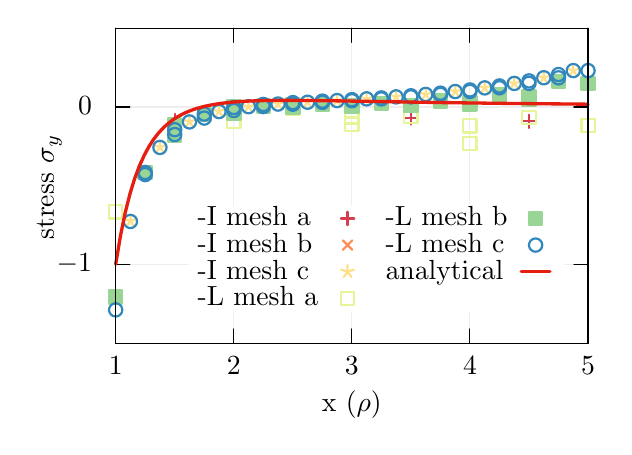
\begin{tikzpicture}[gnuplot]
%% generated with GNUPLOT 5.2p6 (Lua 5.3; terminal rev. Nov 2018, script rev. 107)
%% 03/02/2019 21:03:36
\path (0.000,0.000) rectangle (6.000,4.000);
\gpcolor{rgb color={0.933,0.933,0.933}}
\gpsetlinetype{gp lt border}
\gpsetdashtype{gp dt solid}
\gpsetlinewidth{1.00}
\draw[gp path] (0.000,1.000)--(0.923,1.000);
\draw[gp path] (5.699,1.000)--(5.999,1.000);
\gpcolor{color=gp lt color border}
\draw[gp path] (0.000,1.000)--(0.180,1.000);
\draw[gp path] (5.999,1.000)--(5.819,1.000);
\node[gp node right] at (-0.184,1.000) {$-1$};
\gpcolor{rgb color={0.933,0.933,0.933}}
\draw[gp path] (0.000,2.999)--(5.999,2.999);
\gpcolor{color=gp lt color border}
\draw[gp path] (0.000,2.999)--(0.180,2.999);
\draw[gp path] (5.999,2.999)--(5.819,2.999);
\node[gp node right] at (-0.184,2.999) {$0$};
\gpcolor{rgb color={0.933,0.933,0.933}}
\draw[gp path] (0.000,0.000)--(0.000,3.999);
\gpcolor{color=gp lt color border}
\draw[gp path] (0.000,0.000)--(0.000,0.180);
\draw[gp path] (0.000,3.999)--(0.000,3.819);
\node[gp node center] at (0.000,-0.308) {$1$};
\gpcolor{rgb color={0.933,0.933,0.933}}
\draw[gp path] (1.500,0.000)--(1.500,0.400);
\draw[gp path] (1.500,1.752)--(1.500,3.999);
\gpcolor{color=gp lt color border}
\draw[gp path] (1.500,0.000)--(1.500,0.180);
\draw[gp path] (1.500,3.999)--(1.500,3.819);
\node[gp node center] at (1.500,-0.308) {$2$};
\gpcolor{rgb color={0.933,0.933,0.933}}
\draw[gp path] (3.000,0.000)--(3.000,0.400);
\draw[gp path] (3.000,1.752)--(3.000,3.999);
\gpcolor{color=gp lt color border}
\draw[gp path] (3.000,0.000)--(3.000,0.180);
\draw[gp path] (3.000,3.999)--(3.000,3.819);
\node[gp node center] at (3.000,-0.308) {$3$};
\gpcolor{rgb color={0.933,0.933,0.933}}
\draw[gp path] (4.499,0.000)--(4.499,0.400);
\draw[gp path] (4.499,1.752)--(4.499,3.999);
\gpcolor{color=gp lt color border}
\draw[gp path] (4.499,0.000)--(4.499,0.180);
\draw[gp path] (4.499,3.999)--(4.499,3.819);
\node[gp node center] at (4.499,-0.308) {$4$};
\gpcolor{rgb color={0.933,0.933,0.933}}
\draw[gp path] (5.999,0.000)--(5.999,3.999);
\gpcolor{color=gp lt color border}
\draw[gp path] (5.999,0.000)--(5.999,0.180);
\draw[gp path] (5.999,3.999)--(5.999,3.819);
\node[gp node center] at (5.999,-0.308) {$5$};
\draw[gp path] (0.000,3.999)--(0.000,0.000)--(5.999,0.000)--(5.999,3.999)--cycle;
\node[gp node center,rotate=-270] at (-0.860,1.999) {stress $\sigma_y$};
\node[gp node center] at (2.999,-0.769) {x ($\rho$)};
\node[gp node left] at (0.923,1.583) {-I mesh a};
\gpcolor{rgb color={0.835,0.243,0.310}}
\gpsetlinewidth{2.00}
\gpsetpointsize{6.00}
\gppoint{gp mark 1}{(0.750,2.828)}
\gppoint{gp mark 1}{(2.250,2.990)}
\gppoint{gp mark 1}{(3.749,2.861)}
\gppoint{gp mark 1}{(5.249,2.816)}
\gppoint{gp mark 1}{(2.945,1.583)}
\gpcolor{color=gp lt color border}
\node[gp node left] at (0.923,1.245) {-I mesh b};
\gpcolor{rgb color={0.988,0.553,0.349}}
\gppoint{gp mark 2}{(0.375,2.193)}
\gppoint{gp mark 2}{(1.125,2.914)}
\gppoint{gp mark 2}{(1.875,3.014)}
\gppoint{gp mark 2}{(2.625,3.030)}
\gppoint{gp mark 2}{(3.374,3.040)}
\gppoint{gp mark 2}{(4.124,3.069)}
\gppoint{gp mark 2}{(4.874,3.143)}
\gppoint{gp mark 2}{(5.624,3.314)}
\gppoint{gp mark 2}{(2.945,1.245)}
\gpcolor{color=gp lt color border}
\node[gp node left] at (0.923,0.907) {-I mesh c};
\gpcolor{rgb color={0.996,0.878,0.545}}
\gppoint{gp mark 3}{(0.187,1.551)}
\gppoint{gp mark 3}{(0.562,2.488)}
\gppoint{gp mark 3}{(0.937,2.812)}
\gppoint{gp mark 3}{(1.312,2.943)}
\gppoint{gp mark 3}{(1.687,3.003)}
\gppoint{gp mark 3}{(2.062,3.037)}
\gppoint{gp mark 3}{(2.437,3.060)}
\gppoint{gp mark 3}{(2.812,3.080)}
\gppoint{gp mark 3}{(3.187,3.102)}
\gppoint{gp mark 3}{(3.562,3.127)}
\gppoint{gp mark 3}{(3.937,3.158)}
\gppoint{gp mark 3}{(4.312,3.195)}
\gppoint{gp mark 3}{(4.687,3.241)}
\gppoint{gp mark 3}{(5.062,3.298)}
\gppoint{gp mark 3}{(5.437,3.370)}
\gppoint{gp mark 3}{(5.812,3.460)}
\gppoint{gp mark 3}{(2.945,0.907)}
\gpcolor{color=gp lt color border}
\node[gp node left] at (0.923,0.569) {-L mesh a};
\gpcolor{rgb color={0.902,0.961,0.596}}
\gppoint{gp mark 4}{(0.000,1.666)}
\gppoint{gp mark 4}{(0.750,2.751)}
\gppoint{gp mark 4}{(1.500,2.819)}
\gppoint{gp mark 4}{(1.500,2.977)}
\gppoint{gp mark 4}{(2.250,2.980)}
\gppoint{gp mark 4}{(3.000,2.874)}
\gppoint{gp mark 4}{(3.000,2.781)}
\gppoint{gp mark 4}{(3.749,2.876)}
\gppoint{gp mark 4}{(4.499,2.759)}
\gppoint{gp mark 4}{(4.499,2.537)}
\gppoint{gp mark 4}{(5.249,2.867)}
\gppoint{gp mark 4}{(5.999,2.766)}
\gppoint{gp mark 4}{(2.945,0.569)}
\gpcolor{color=gp lt color border}
\node[gp node left] at (3.311,1.583) {-L mesh b};
\gpcolor{rgb color={0.600,0.835,0.580}}
\gppoint{gp mark 5}{(0.000,0.586)}
\gppoint{gp mark 5}{(0.375,2.167)}
\gppoint{gp mark 5}{(0.750,2.637)}
\gppoint{gp mark 5}{(0.750,2.775)}
\gppoint{gp mark 5}{(1.125,2.904)}
\gppoint{gp mark 5}{(1.500,2.921)}
\gppoint{gp mark 5}{(1.500,3.003)}
\gppoint{gp mark 5}{(1.875,3.010)}
\gppoint{gp mark 5}{(2.250,2.989)}
\gppoint{gp mark 5}{(2.250,3.022)}
\gppoint{gp mark 5}{(2.625,3.029)}
\gppoint{gp mark 5}{(3.000,3.005)}
\gppoint{gp mark 5}{(3.000,3.016)}
\gppoint{gp mark 5}{(3.374,3.040)}
\gppoint{gp mark 5}{(3.749,3.018)}
\gppoint{gp mark 5}{(3.749,3.018)}
\gppoint{gp mark 5}{(4.124,3.072)}
\gppoint{gp mark 5}{(4.499,3.050)}
\gppoint{gp mark 5}{(4.499,3.038)}
\gppoint{gp mark 5}{(4.874,3.148)}
\gppoint{gp mark 5}{(5.249,3.125)}
\gppoint{gp mark 5}{(5.249,3.094)}
\gppoint{gp mark 5}{(5.624,3.322)}
\gppoint{gp mark 5}{(5.999,3.299)}
\gppoint{gp mark 5}{(5.333,1.583)}
\gpcolor{color=gp lt color border}
\node[gp node left] at (3.311,1.245) {-L mesh c};
\gpcolor{rgb color={0.196,0.533,0.741}}
\gppoint{gp mark 6}{(0.000,0.422)}
\gppoint{gp mark 6}{(0.187,1.545)}
\gppoint{gp mark 6}{(0.375,2.140)}
\gppoint{gp mark 6}{(0.375,2.167)}
\gppoint{gp mark 6}{(0.562,2.485)}
\gppoint{gp mark 6}{(0.750,2.649)}
\gppoint{gp mark 6}{(0.750,2.710)}
\gppoint{gp mark 6}{(0.937,2.809)}
\gppoint{gp mark 6}{(1.125,2.858)}
\gppoint{gp mark 6}{(1.125,2.909)}
\gppoint{gp mark 6}{(1.312,2.941)}
\gppoint{gp mark 6}{(1.500,2.954)}
\gppoint{gp mark 6}{(1.500,2.992)}
\gppoint{gp mark 6}{(1.687,3.002)}
\gppoint{gp mark 6}{(1.875,3.004)}
\gppoint{gp mark 6}{(1.875,3.031)}
\gppoint{gp mark 6}{(2.062,3.036)}
\gppoint{gp mark 6}{(2.250,3.034)}
\gppoint{gp mark 6}{(2.250,3.054)}
\gppoint{gp mark 6}{(2.437,3.059)}
\gppoint{gp mark 6}{(2.625,3.057)}
\gppoint{gp mark 6}{(2.625,3.073)}
\gppoint{gp mark 6}{(2.812,3.080)}
\gppoint{gp mark 6}{(3.000,3.078)}
\gppoint{gp mark 6}{(3.000,3.092)}
\gppoint{gp mark 6}{(3.187,3.102)}
\gppoint{gp mark 6}{(3.374,3.101)}
\gppoint{gp mark 6}{(3.374,3.114)}
\gppoint{gp mark 6}{(3.562,3.127)}
\gppoint{gp mark 6}{(3.749,3.127)}
\gppoint{gp mark 6}{(3.749,3.141)}
\gppoint{gp mark 6}{(3.937,3.158)}
\gppoint{gp mark 6}{(4.124,3.158)}
\gppoint{gp mark 6}{(4.124,3.174)}
\gppoint{gp mark 6}{(4.312,3.195)}
\gppoint{gp mark 6}{(4.499,3.196)}
\gppoint{gp mark 6}{(4.499,3.215)}
\gppoint{gp mark 6}{(4.687,3.241)}
\gppoint{gp mark 6}{(4.874,3.242)}
\gppoint{gp mark 6}{(4.874,3.266)}
\gppoint{gp mark 6}{(5.062,3.298)}
\gppoint{gp mark 6}{(5.249,3.299)}
\gppoint{gp mark 6}{(5.249,3.330)}
\gppoint{gp mark 6}{(5.437,3.370)}
\gppoint{gp mark 6}{(5.624,3.369)}
\gppoint{gp mark 6}{(5.624,3.411)}
\gppoint{gp mark 6}{(5.812,3.461)}
\gppoint{gp mark 6}{(5.999,3.461)}
\gppoint{gp mark 6}{(5.333,1.245)}
\gpcolor{color=gp lt color border}
\node[gp node left] at (3.311,0.907) {analytical};
\gpcolor{rgb color={0.898,0.118,0.063}}
\gpsetlinewidth{3.00}
\draw[gp path] (5.151,0.907)--(5.515,0.907);
\draw[gp path] (0.000,1.000)--(0.061,1.363)--(0.121,1.657)--(0.182,1.897)--(0.242,2.093)%
  --(0.303,2.254)--(0.364,2.388)--(0.424,2.499)--(0.485,2.592)--(0.545,2.669)--(0.606,2.735)%
  --(0.667,2.789)--(0.727,2.836)--(0.788,2.875)--(0.848,2.908)--(0.909,2.936)--(0.970,2.960)%
  --(1.030,2.980)--(1.091,2.997)--(1.151,3.012)--(1.212,3.024)--(1.273,3.035)--(1.333,3.044)%
  --(1.394,3.051)--(1.454,3.058)--(1.515,3.063)--(1.575,3.067)--(1.636,3.071)--(1.697,3.074)%
  --(1.757,3.076)--(1.818,3.078)--(1.878,3.080)--(1.939,3.081)--(2.000,3.082)--(2.060,3.082)%
  --(2.121,3.082)--(2.181,3.083)--(2.242,3.082)--(2.303,3.082)--(2.363,3.082)--(2.424,3.081)%
  --(2.484,3.081)--(2.545,3.080)--(2.606,3.079)--(2.666,3.078)--(2.727,3.078)--(2.787,3.077)%
  --(2.848,3.076)--(2.909,3.075)--(2.969,3.074)--(3.030,3.073)--(3.090,3.072)--(3.151,3.071)%
  --(3.212,3.070)--(3.272,3.069)--(3.333,3.068)--(3.393,3.067)--(3.454,3.066)--(3.515,3.065)%
  --(3.575,3.064)--(3.636,3.063)--(3.696,3.062)--(3.757,3.061)--(3.818,3.060)--(3.878,3.059)%
  --(3.939,3.058)--(3.999,3.057)--(4.060,3.056)--(4.121,3.055)--(4.181,3.054)--(4.242,3.054)%
  --(4.302,3.053)--(4.363,3.052)--(4.424,3.051)--(4.484,3.050)--(4.545,3.049)--(4.605,3.049)%
  --(4.666,3.048)--(4.726,3.047)--(4.787,3.046)--(4.848,3.046)--(4.908,3.045)--(4.969,3.044)%
  --(5.029,3.044)--(5.090,3.043)--(5.151,3.042)--(5.211,3.042)--(5.272,3.041)--(5.332,3.040)%
  --(5.393,3.040)--(5.454,3.039)--(5.514,3.039)--(5.575,3.038)--(5.635,3.038)--(5.696,3.037)%
  --(5.757,3.036)--(5.817,3.036)--(5.878,3.035)--(5.938,3.035)--(5.999,3.034);
\gpcolor{color=gp lt color border}
\gpsetlinewidth{1.00}
\draw[gp path] (0.000,3.999)--(0.000,0.000)--(5.999,0.000)--(5.999,3.999)--cycle;
%% coordinates of the plot area
\gpdefrectangularnode{gp plot 1}{\pgfpoint{0.000cm}{0.000cm}}{\pgfpoint{5.999cm}{3.999cm}}
\end{tikzpicture}
%% gnuplot variables

\caption{vertical stress $\sigma_y$ distribution at $y=0$}
\end{subfigure}\quad
\begin{subfigure}[b]{.49\textwidth}\centering
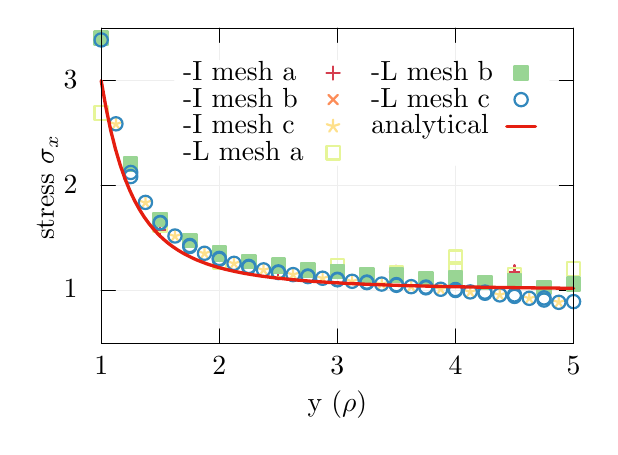
\begin{tikzpicture}[gnuplot]
%% generated with GNUPLOT 5.2p6 (Lua 5.3; terminal rev. Nov 2018, script rev. 107)
%% 03/02/2019 21:03:33
\path (0.000,0.000) rectangle (6.000,4.000);
\gpcolor{rgb color={0.933,0.933,0.933}}
\gpsetlinetype{gp lt border}
\gpsetdashtype{gp dt solid}
\gpsetlinewidth{1.00}
\draw[gp path] (0.000,0.667)--(5.999,0.667);
\gpcolor{color=gp lt color border}
\draw[gp path] (0.000,0.667)--(0.180,0.667);
\draw[gp path] (5.999,0.667)--(5.819,0.667);
\node[gp node right] at (-0.184,0.667) {$1$};
\gpcolor{rgb color={0.933,0.933,0.933}}
\draw[gp path] (0.000,2.000)--(5.999,2.000);
\gpcolor{color=gp lt color border}
\draw[gp path] (0.000,2.000)--(0.180,2.000);
\draw[gp path] (5.999,2.000)--(5.819,2.000);
\node[gp node right] at (-0.184,2.000) {$2$};
\gpcolor{rgb color={0.933,0.933,0.933}}
\draw[gp path] (0.000,3.333)--(0.923,3.333);
\draw[gp path] (5.699,3.333)--(5.999,3.333);
\gpcolor{color=gp lt color border}
\draw[gp path] (0.000,3.333)--(0.180,3.333);
\draw[gp path] (5.999,3.333)--(5.819,3.333);
\node[gp node right] at (-0.184,3.333) {$3$};
\gpcolor{rgb color={0.933,0.933,0.933}}
\draw[gp path] (0.000,0.000)--(0.000,3.999);
\gpcolor{color=gp lt color border}
\draw[gp path] (0.000,0.000)--(0.000,0.180);
\draw[gp path] (0.000,3.999)--(0.000,3.819);
\node[gp node center] at (0.000,-0.308) {$1$};
\gpcolor{rgb color={0.933,0.933,0.933}}
\draw[gp path] (1.500,0.000)--(1.500,2.247);
\draw[gp path] (1.500,3.599)--(1.500,3.999);
\gpcolor{color=gp lt color border}
\draw[gp path] (1.500,0.000)--(1.500,0.180);
\draw[gp path] (1.500,3.999)--(1.500,3.819);
\node[gp node center] at (1.500,-0.308) {$2$};
\gpcolor{rgb color={0.933,0.933,0.933}}
\draw[gp path] (3.000,0.000)--(3.000,2.247);
\draw[gp path] (3.000,3.599)--(3.000,3.999);
\gpcolor{color=gp lt color border}
\draw[gp path] (3.000,0.000)--(3.000,0.180);
\draw[gp path] (3.000,3.999)--(3.000,3.819);
\node[gp node center] at (3.000,-0.308) {$3$};
\gpcolor{rgb color={0.933,0.933,0.933}}
\draw[gp path] (4.499,0.000)--(4.499,2.247);
\draw[gp path] (4.499,3.599)--(4.499,3.999);
\gpcolor{color=gp lt color border}
\draw[gp path] (4.499,0.000)--(4.499,0.180);
\draw[gp path] (4.499,3.999)--(4.499,3.819);
\node[gp node center] at (4.499,-0.308) {$4$};
\gpcolor{rgb color={0.933,0.933,0.933}}
\draw[gp path] (5.999,0.000)--(5.999,3.999);
\gpcolor{color=gp lt color border}
\draw[gp path] (5.999,0.000)--(5.999,0.180);
\draw[gp path] (5.999,3.999)--(5.999,3.819);
\node[gp node center] at (5.999,-0.308) {$5$};
\draw[gp path] (0.000,3.999)--(0.000,0.000)--(5.999,0.000)--(5.999,3.999)--cycle;
\node[gp node center,rotate=-270] at (-0.676,1.999) {stress $\sigma_x$};
\node[gp node center] at (2.999,-0.769) {y ($\rho$)};
\node[gp node left] at (0.923,3.430) {-I mesh a};
\gpcolor{rgb color={0.835,0.243,0.310}}
\gpsetlinewidth{2.00}
\gpsetpointsize{6.00}
\gppoint{gp mark 1}{(0.750,1.437)}
\gppoint{gp mark 1}{(2.250,0.911)}
\gppoint{gp mark 1}{(3.749,0.900)}
\gppoint{gp mark 1}{(5.249,0.906)}
\gppoint{gp mark 1}{(2.945,3.430)}
\gpcolor{color=gp lt color border}
\node[gp node left] at (0.923,3.092) {-I mesh b};
\gpcolor{rgb color={0.988,0.553,0.349}}
\gppoint{gp mark 2}{(0.375,2.259)}
\gppoint{gp mark 2}{(1.125,1.294)}
\gppoint{gp mark 2}{(1.875,1.036)}
\gppoint{gp mark 2}{(2.625,0.929)}
\gppoint{gp mark 2}{(3.374,0.868)}
\gppoint{gp mark 2}{(4.124,0.820)}
\gppoint{gp mark 2}{(4.874,0.771)}
\gppoint{gp mark 2}{(5.624,0.711)}
\gppoint{gp mark 2}{(2.945,3.092)}
\gpcolor{color=gp lt color border}
\node[gp node left] at (0.923,2.754) {-I mesh c};
\gpcolor{rgb color={0.996,0.878,0.545}}
\gppoint{gp mark 3}{(0.187,2.781)}
\gppoint{gp mark 3}{(0.562,1.784)}
\gppoint{gp mark 3}{(0.937,1.358)}
\gppoint{gp mark 3}{(1.312,1.140)}
\gppoint{gp mark 3}{(1.687,1.012)}
\gppoint{gp mark 3}{(2.062,0.929)}
\gppoint{gp mark 3}{(2.437,0.870)}
\gppoint{gp mark 3}{(2.812,0.824)}
\gppoint{gp mark 3}{(3.187,0.785)}
\gppoint{gp mark 3}{(3.562,0.750)}
\gppoint{gp mark 3}{(3.937,0.718)}
\gppoint{gp mark 3}{(4.312,0.685)}
\gppoint{gp mark 3}{(4.687,0.650)}
\gppoint{gp mark 3}{(5.062,0.612)}
\gppoint{gp mark 3}{(5.437,0.569)}
\gppoint{gp mark 3}{(5.812,0.519)}
\gppoint{gp mark 3}{(2.945,2.754)}
\gpcolor{color=gp lt color border}
\node[gp node left] at (0.923,2.416) {-L mesh a};
\gpcolor{rgb color={0.902,0.961,0.596}}
\gppoint{gp mark 4}{(0.000,2.922)}
\gppoint{gp mark 4}{(0.750,1.500)}
\gppoint{gp mark 4}{(1.500,1.039)}
\gppoint{gp mark 4}{(1.500,1.031)}
\gppoint{gp mark 4}{(2.250,0.919)}
\gppoint{gp mark 4}{(3.000,0.908)}
\gppoint{gp mark 4}{(3.000,0.984)}
\gppoint{gp mark 4}{(3.749,0.890)}
\gppoint{gp mark 4}{(4.499,0.942)}
\gppoint{gp mark 4}{(4.499,1.093)}
\gppoint{gp mark 4}{(5.249,0.872)}
\gppoint{gp mark 4}{(5.999,0.941)}
\gppoint{gp mark 4}{(2.945,2.416)}
\gpcolor{color=gp lt color border}
\node[gp node left] at (3.311,3.430) {-L mesh b};
\gpcolor{rgb color={0.600,0.835,0.580}}
\gppoint{gp mark 5}{(0.000,3.873)}
\gppoint{gp mark 5}{(0.375,2.277)}
\gppoint{gp mark 5}{(0.750,1.567)}
\gppoint{gp mark 5}{(0.750,1.567)}
\gppoint{gp mark 5}{(1.125,1.300)}
\gppoint{gp mark 5}{(1.500,1.151)}
\gppoint{gp mark 5}{(1.500,1.126)}
\gppoint{gp mark 5}{(1.875,1.039)}
\gppoint{gp mark 5}{(2.250,0.989)}
\gppoint{gp mark 5}{(2.250,0.979)}
\gppoint{gp mark 5}{(2.625,0.930)}
\gppoint{gp mark 5}{(3.000,0.912)}
\gppoint{gp mark 5}{(3.000,0.908)}
\gppoint{gp mark 5}{(3.374,0.868)}
\gppoint{gp mark 5}{(3.749,0.864)}
\gppoint{gp mark 5}{(3.749,0.863)}
\gppoint{gp mark 5}{(4.124,0.819)}
\gppoint{gp mark 5}{(4.499,0.826)}
\gppoint{gp mark 5}{(4.499,0.826)}
\gppoint{gp mark 5}{(4.874,0.767)}
\gppoint{gp mark 5}{(5.249,0.789)}
\gppoint{gp mark 5}{(5.249,0.793)}
\gppoint{gp mark 5}{(5.624,0.704)}
\gppoint{gp mark 5}{(5.999,0.750)}
\gppoint{gp mark 5}{(5.333,3.430)}
\gpcolor{color=gp lt color border}
\node[gp node left] at (3.311,3.092) {-L mesh c};
\gpcolor{rgb color={0.196,0.533,0.741}}
\gppoint{gp mark 6}{(0.000,3.850)}
\gppoint{gp mark 6}{(0.187,2.785)}
\gppoint{gp mark 6}{(0.375,2.115)}
\gppoint{gp mark 6}{(0.375,2.167)}
\gppoint{gp mark 6}{(0.562,1.787)}
\gppoint{gp mark 6}{(0.750,1.531)}
\gppoint{gp mark 6}{(0.750,1.527)}
\gppoint{gp mark 6}{(0.937,1.360)}
\gppoint{gp mark 6}{(1.125,1.240)}
\gppoint{gp mark 6}{(1.125,1.227)}
\gppoint{gp mark 6}{(1.312,1.141)}
\gppoint{gp mark 6}{(1.500,1.076)}
\gppoint{gp mark 6}{(1.500,1.064)}
\gppoint{gp mark 6}{(1.687,1.013)}
\gppoint{gp mark 6}{(1.875,0.974)}
\gppoint{gp mark 6}{(1.875,0.964)}
\gppoint{gp mark 6}{(2.062,0.930)}
\gppoint{gp mark 6}{(2.250,0.904)}
\gppoint{gp mark 6}{(2.250,0.896)}
\gppoint{gp mark 6}{(2.437,0.870)}
\gppoint{gp mark 6}{(2.625,0.852)}
\gppoint{gp mark 6}{(2.625,0.845)}
\gppoint{gp mark 6}{(2.812,0.824)}
\gppoint{gp mark 6}{(3.000,0.810)}
\gppoint{gp mark 6}{(3.000,0.804)}
\gppoint{gp mark 6}{(3.187,0.785)}
\gppoint{gp mark 6}{(3.374,0.775)}
\gppoint{gp mark 6}{(3.374,0.768)}
\gppoint{gp mark 6}{(3.562,0.750)}
\gppoint{gp mark 6}{(3.749,0.743)}
\gppoint{gp mark 6}{(3.749,0.734)}
\gppoint{gp mark 6}{(3.937,0.717)}
\gppoint{gp mark 6}{(4.124,0.712)}
\gppoint{gp mark 6}{(4.124,0.702)}
\gppoint{gp mark 6}{(4.312,0.684)}
\gppoint{gp mark 6}{(4.499,0.681)}
\gppoint{gp mark 6}{(4.499,0.668)}
\gppoint{gp mark 6}{(4.687,0.650)}
\gppoint{gp mark 6}{(4.874,0.648)}
\gppoint{gp mark 6}{(4.874,0.633)}
\gppoint{gp mark 6}{(5.062,0.612)}
\gppoint{gp mark 6}{(5.249,0.613)}
\gppoint{gp mark 6}{(5.249,0.593)}
\gppoint{gp mark 6}{(5.437,0.569)}
\gppoint{gp mark 6}{(5.624,0.574)}
\gppoint{gp mark 6}{(5.624,0.547)}
\gppoint{gp mark 6}{(5.812,0.518)}
\gppoint{gp mark 6}{(5.999,0.527)}
\gppoint{gp mark 6}{(5.333,3.092)}
\gpcolor{color=gp lt color border}
\node[gp node left] at (3.311,2.754) {analytical};
\gpcolor{rgb color={0.898,0.118,0.063}}
\gpsetlinewidth{3.00}
\draw[gp path] (5.151,2.754)--(5.515,2.754);
\draw[gp path] (0.000,3.333)--(0.061,2.989)--(0.121,2.702)--(0.182,2.462)--(0.242,2.259)%
  --(0.303,2.086)--(0.364,1.937)--(0.424,1.810)--(0.485,1.699)--(0.545,1.603)--(0.606,1.519)%
  --(0.667,1.445)--(0.727,1.380)--(0.788,1.322)--(0.848,1.271)--(0.909,1.225)--(0.970,1.184)%
  --(1.030,1.148)--(1.091,1.115)--(1.151,1.085)--(1.212,1.057)--(1.273,1.033)--(1.333,1.010)%
  --(1.394,0.990)--(1.454,0.971)--(1.515,0.954)--(1.575,0.938)--(1.636,0.924)--(1.697,0.910)%
  --(1.757,0.898)--(1.818,0.886)--(1.878,0.876)--(1.939,0.866)--(2.000,0.856)--(2.060,0.848)%
  --(2.121,0.840)--(2.181,0.832)--(2.242,0.825)--(2.303,0.819)--(2.363,0.812)--(2.424,0.807)%
  --(2.484,0.801)--(2.545,0.796)--(2.606,0.791)--(2.666,0.786)--(2.727,0.782)--(2.787,0.778)%
  --(2.848,0.774)--(2.909,0.770)--(2.969,0.767)--(3.030,0.764)--(3.090,0.760)--(3.151,0.757)%
  --(3.212,0.755)--(3.272,0.752)--(3.333,0.749)--(3.393,0.747)--(3.454,0.744)--(3.515,0.742)%
  --(3.575,0.740)--(3.636,0.738)--(3.696,0.736)--(3.757,0.734)--(3.818,0.732)--(3.878,0.730)%
  --(3.939,0.729)--(3.999,0.727)--(4.060,0.726)--(4.121,0.724)--(4.181,0.723)--(4.242,0.721)%
  --(4.302,0.720)--(4.363,0.719)--(4.424,0.717)--(4.484,0.716)--(4.545,0.715)--(4.605,0.714)%
  --(4.666,0.713)--(4.726,0.712)--(4.787,0.711)--(4.848,0.710)--(4.908,0.709)--(4.969,0.708)%
  --(5.029,0.707)--(5.090,0.706)--(5.151,0.706)--(5.211,0.705)--(5.272,0.704)--(5.332,0.703)%
  --(5.393,0.703)--(5.454,0.702)--(5.514,0.701)--(5.575,0.700)--(5.635,0.700)--(5.696,0.699)%
  --(5.757,0.699)--(5.817,0.698)--(5.878,0.697)--(5.938,0.697)--(5.999,0.696);
\gpcolor{color=gp lt color border}
\gpsetlinewidth{1.00}
\draw[gp path] (0.000,3.999)--(0.000,0.000)--(5.999,0.000)--(5.999,3.999)--cycle;
%% coordinates of the plot area
\gpdefrectangularnode{gp plot 1}{\pgfpoint{0.000cm}{0.000cm}}{\pgfpoint{5.999cm}{3.999cm}}
\end{tikzpicture}
%% gnuplot variables

\caption{horizontal stress $\sigma_x$ distribution at $x=0$}
\end{subfigure}
\caption{stress prediction for plate with circular hole}\label{fig:plate_with_hole_stress}
\end{figure}
Due to finite element discretization, the exact Kirsch's solution \textbf{cannot} be obtained. However, numerical results stay close to analytical one and with mesh b, a decent result is obtained. Mesh a is simply too coarse to map \eqsref{kirsch_a} and \eqsref{kirsch_b}. Though, the error is still bounded within a reasonable range. The work by \citet{Madeo2014} is referred to here for more comparisons between numerical and analytical solutions.

Furthermore, as mesh grid becomes denser, GCMQ-I tends to produce the same stress field as of GCMQ-L. This means, if a dense mesh grid is used, analysts could consider to use GCMQ-I instead of GCMQ-L for better efficiency, if stability is not an issue. Compared to traditional displacement based elements, as there is no additional treatment required for recovering strain and stress fields, GCMQ omits uncertainties that exist in most strain/stress averaging methods, which often lead to less accurate results by their nature, and further simplifies numerical analysis work flow. For a moderately smooth stress distribution, it can be seen that the interpolated field is reasonable and relatively accurate even with a coarse mesh grid. However, for an extremely discontinuous stress field, which is quite common in elasto-plastic cases, point-wise accurate stress field is in general not achievable without mesh refinement. This statement is valid for all finite elements.
\section{Conclusions}
In this work, a new variational framework based on the Hu-Washizu variational principle is established. It supports the handling of different displacement and strain components. Based on this framework, a high-performing four-node drilling membrane element, named as GCMQ, that combines advantages of both mixed formulation and generalized conforming approach, is proposed. It has been shown that the generalized conforming concept, which is originally developed based on a modified minimum potential energy theorem \citep{Long2009}, can also be extended to a mixed formulation. The overall performance of the proposed element is better than most other similar elements, hence it can be counted as one of the top-performing four-node elements.

The following strategies are used in design of GCMQ:
\begin{enumerate}
\item Given that a displacement-based approach tends to be too stiff, a mixed formulation based on the modified Hu-Washizu variational principle is adopted to produce softer response.
\item Instead of increasing element nodes, the drilling DoFs are included to grant GCMQ the ability of describing a non-linear displacement field and address the connectivity issue with other types of elements.
\item Stress and strain are constructed based on complete quadratic polynomials to cover more stress and strain patterns.
\item The auxiliary field, enhanced strain, is fine-tuned via numerical experiments to improve the performance.
\end{enumerate}

With the presence of drilling DoFs and mixed framework, the proposed GCMQ element could be used in both simple and complex models with elastoplastic materials. It could be concluded that with the same mesh configuration, compared with other similar elements, the proposed GCMQ element can predict better results and is less sensitive to slight/moderate mesh distortion. The element is also free from shear locking and volumetric locking. Meanwhile, since stress and strain fields are explicitly interpolated in GCMQ, analysts can directly recover stress and strain distributions using interpolation parameters so that unreliable extrapolation methods can be avoided.

For efficiency, a modified five-point integration scheme is proposed to minimise computational cost. It can be seen that such a scheme is accurate for general linear applications but is sensitive to severe mesh distortion. In that case, analysts are recommended to use a \numproduct{3x3} Lobatto quadrature. It could also be observed from examples that the performance of GCMQ is consistently slightly stiffer than the true solution. It shall be noted that no empirical artificial parameter that may affect the performance exists in the presented formulation.

The GCMQ element has been implemented in \texttt{suanPan} \citep{Chang2018}. All examples used in this paper can be found online\footnote{https://github.com/TLCFEM/gcmq-ijnme}. It is also available as a dynamic link library on the finite element analysis platform OpenSees\footnote{http://opensees.berkeley.edu/}. The binary files and source code can be downloaded from the corresponding repository\footnote{https://github.com/TLCFEM/gcmq-opensees-implementation}.
\section*{Acknowledgement}
The authors would like to acknowledge the financial support under grant number E6953 provided by the Earthquake Commission\footnote{https://www.eqc.govt.nz/} (EQC).
\bibliography{FORMULATION}
\end{document}